\documentclass[10pt]{article}
\usepackage{commands}
\usepackage{slashed}
\usepackage{pxfonts}
\pgfplotsset{compat=1.18}

\begin{document}
\begin{tcolorbox}
  \begin{center}
  \begin{Large}
    \textbf{PHYS 411 (Topics in Many-Body Dynamics) Notes} \\
    \vspace{5pt}
  \end{Large}
  \begin{large}
        Rio Weil \\
\vspace{5pt}
    \emph{This document was typeset on \today}
  \end{large}
  \end{center}
\end{tcolorbox}

\begin{center}
  \textbf{Introduction:}

  This is a set of lecture notes taken from UChicago's PHYS 411 (Topics in Many-Body Dynamics), taught by Vincenzo Vitelli. Topics covered include Continuum Mechanics, Classification of Elastic Moduli, Odd Elastodynamics, Self-Propelled Particles, Odd Viscosity, Turbulence, Active Brownian Motion and MIPS, Pattern Formation, and Non-Reciprocal Phase Transitions.
\end{center}
\addtocontents{toc}{\protect\hypertarget{toc}{}}
\tableofcontents

\newpage
\section{Continuum Mechanics}

\subsection{Course Overview}
This course is a topics course in many-body dynamics. What does that mean? It is inspired by a Polykov used to teach in Princeton, called ``Topics'', where he would arrive 10 minutes before and decide what would be an important topic in theoretical physics to teach. I (Vincenzo) don't have quite this level of improvisation, but this will largely be a course in research topics of non-equilibrium many-body physics/active matter.

We do have a broad theme - we want to treat various aspects of physics (mechanics, solid physics, phase transitions) from the perspective of dynamical systems. The formal pre-reqs are the intro soft matter course (currently being taught in parallel) as well as a course in statical field theory, but these are in some sense excessive - an enterprising student would be able to follow along, with some additional reading.

There is a recommended book (Soft Matter by Vitelli and others). The book will make the lectures look good in that the lectures will have better explanations. But since this course is being taught for the first time, there will be no lecture notes, so some sections of the book may be useful.

Assessment will be from problem sets (3 problem sets of 3-4 problems each). They may be difficult (they will be taken from the book) and long, but they will be stimulating and well written out. They will largely be mini research topics (it will be like working on research with a soft matter theorist like me (Vincenzo), or perhaps someone less crazy) - the grading will be lenient accordingly, as well as policies around deadlines, working together.

\subsection{Continuum Mechanics Review}

We will start by looking at equilibrium theory of physics, by looking at elasticity. This is normally a problem treated in the context of variational classical field theory. But we will approach this problem from a non-variational perspective (odd elasticity), and we will see interesting phenomena - namely chaos - emerge.

Our starting point is Newton's second law:
\begin{equation}
    \v{F} = \dod{\v{p}}{t}
\end{equation}

For continuous media, we can consider the force as coming from a volume integral of the pressure over space:
\begin{equation}
    f_i = \dod{}{t}\iiint dV P_i = \oiint dA \sigma_{ij}n_j
\end{equation}
where we have used Stoke's theorem to rewrite the volume integral as an integral over the area. 

\begin{center}
    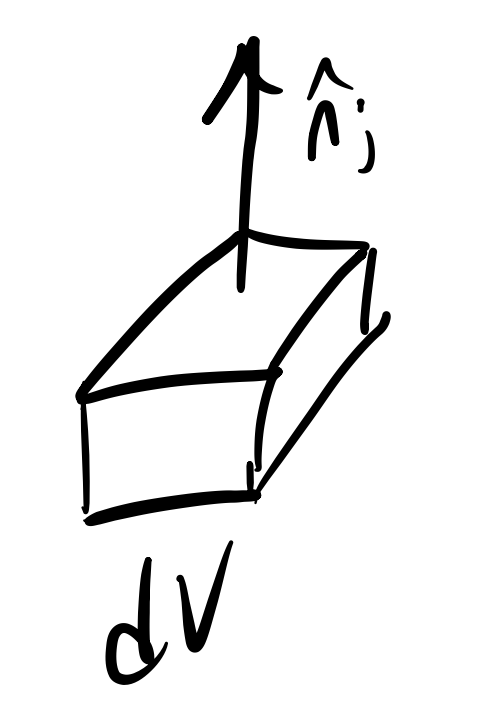
\includegraphics[scale=0.35]{Lectures/Images/lec1-volelement.png}
\end{center}

Therein, $\sigma_{ij}$ is the linear momentum flux, or a rank-2 stress tensor. Note that throughout, we use Einstein summation convention where repeated indices are summed over (e.g. $u_{ij}x_j \coloneqq \sum_j u_{ij}x_j$).

We can further write:
\begin{equation}
    f_i = \iiint \dpd{\sigma_{ij}}{x_j}dV
\end{equation}
Another way to package this; we can write the force as a volume integral of a force density, which is a divergence of the stress tensor:
\begin{equation}
    f_i = \iiint dV F_i
\end{equation}
with:
\begin{equation}\label{eq:forcedensity}
    \boxed{F_i = \p_j \sigma_{ij}}
\end{equation}
one can also take this as the definition of the stress tensor. If you have never seen the stress-tensor, it is recommended you read the first chapter of Soft Matter.

There is an assumption we made here. When we set the volume integral of $dVP_i$ equal to the area integral, we assumed that there were no sources. We will see what happens soon when this assumption is violated. For example we may have a solid immersed in a fluid, in which case Newton's third law may not hold and linear momentum is generically not conserved. One thing that this class will emphasize is what happens to the conclusions when assumptions are challenged!

Let's look at a differential of the force density:
\begin{equation}
    dF_i = \sigma_{ij}n_j dA
\end{equation}
As a concrete example, we can look at the forces acting on different faces of our cube:

\begin{center}
    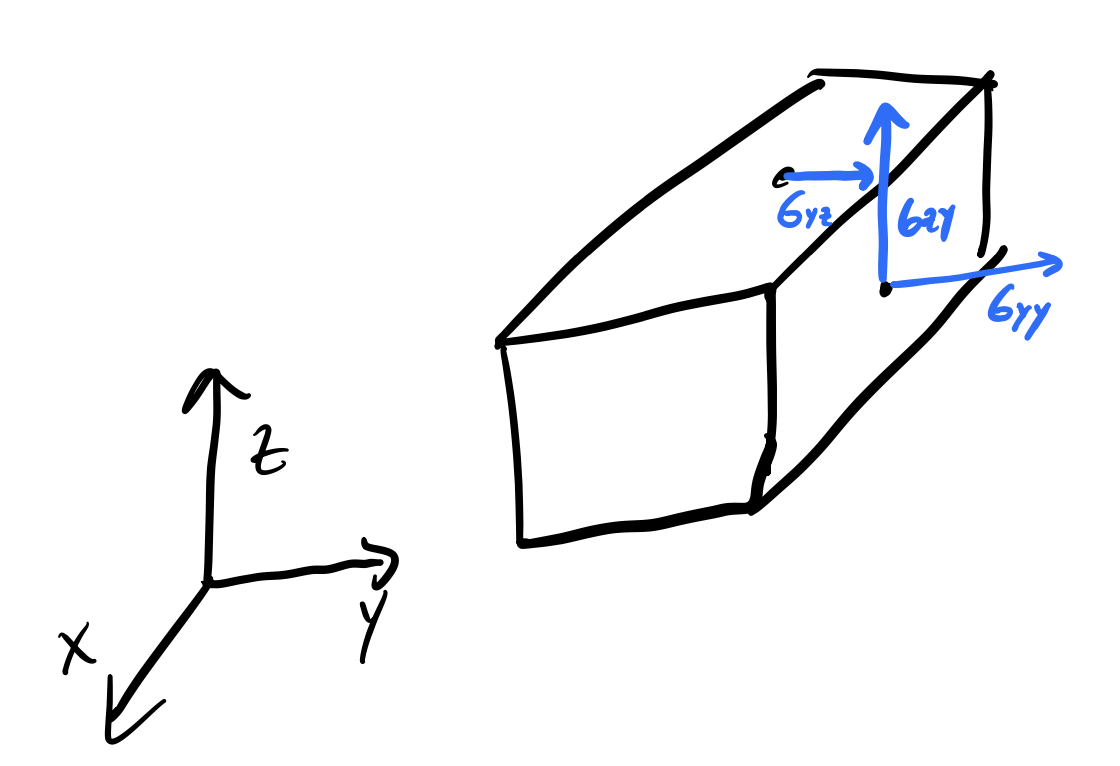
\includegraphics[scale=0.35]{Lectures/Images/lec1-forces.png}
\end{center}

\subsection{Constitutive Equation and Conservation Laws}
We want a relationship between the stress tensor and the order parameter, relating to the displacements. We assume that there is translation invariance for now, so there is no dependence on the displacements themselves, only on gradients of the displacements (this is not true always, e.g. in the case of a solid in fluid, or a solid on a table with glue - these will be additional terms that we consider later). In linear response theory, we connect the stress and strain tensors (rank-2) via a stiffness tensor (rank-4):
\begin{equation}
    \sigma_{ij} = K_{ijkl}\p_k u_l = K_{ijkl}u_{kl}
\end{equation}
The above is a linearized constitutive equation. As ugly as the $K_{ijkl}$ above may be, forms the identity of the material. This is ``Hooke's Law on steroids''. Note that if we assume that microscopically a solid is composed of masses connected by Hookian springs with spring constant $k$, it is possible to derive the macroscopic stiffness tensor from the microscopic theory; this may be one of your problems later.

In 2-D, we have:
\begin{equation}
    u_{kl} = \m{\p_x u_x & \p_x u_y \\ \p_y u_x & \p_y u_y}
\end{equation}
\begin{equation}
    \sigma_{ij} = \m{\sigma_{xx} & \sigma_{xy} \\ \sigma_{yx} & \sigma_{yy}}
\end{equation}
Note that we do not symmetrize here. In fact we can explicitly think about what happens in the cases when the off-diagonal entries are not equal. When $\sigma_{ij} \neq \sigma_{ji}$, it means that there is a non-vanishing net-torque (imagine back to the forces on the cube picture) and so the medium can spontaneously rotate. What does this teach us? Buried in the cumbersome algebraic structure of the rank-4 tensor, we see the presence and or violation of conservation laws. In this case, $\sigma_{ij} \neq \sigma_{ji}$ it implies that angular momentum is \emph{not} conserved. Most books assume the fundamental conservation laws of nature hold and write down theories accordingly. But, we can allow for exotic mechanisms of the breaking of such fundamental laws, e.g. from interactions with external sources which give rise to effective theories.

We are rapidly marching through conservation laws; we have imposed conservation of linear momentum from the get-go, but we do not impose $\sigma_{ij} = \sigma_{ji}$/impose angular momentum conservation (If we did, then the rank-4 tensor would reduce to rank-3). This means that we have external torques present/sources of angular momentum. As we go on, we will study symmetries of our system through the symmetries of the (admittedly complicated) $K_{ijkl}$ object, and understand the conservation laws through it.

Now, we \emph{assume} that there is a potential energy. In Hooke's law, we assume $F = -\p_x E$ with $E = \frac{1}{2}kx^2$ so we have a conservative force. Here, we don't work on the level of single particles, so we write the total potential energy as the integral over energy density:
\begin{equation}
    U = \iiint d^3x \e(\v{x})
\end{equation}
The question is now what is $\e(\v{x})$? If we want a linear force, we require that $\e(\v{x})$ be a quadratic form in $\v{x}$:
\begin{equation}
    \e(\v{x}) = \frac{1}{2}c_{ijkl} u_{ij}(\v{x})u_{kl}(\v{x})
\end{equation}
Now, we want the force in the $l$th direction, which is a functional derivative of the energy density:
\begin{equation}
    \left(\text{Force}\right)_l = -\frac{\delta \e}{\delta u_l} = -\left(\dpd{\e}{u_l} - \p_k \dpd{\e}{u_{lk}}\right)
\end{equation}
where again we recall $u_{lk} = \p_l u_k$. Let's try to unweird this expression via analogy (maybe you want to explain to a friend, or pick up someone at a bar by telling them that you work on functional derivatives) - in classical mechanics, we have an action:
\begin{equation}
    S = \int L(q(t))dt
\end{equation}
we then have the trajectory that is followed is that for which the functional derivative of the action vanishes\footnote{Of course, this is something your date is expected to know.}:
\begin{equation}
    \frac{\delta S}{\delta q} = 0 \implies \dpd{L}{q_j} - \dod{}{t}\left(\dpd{L}{\dot{q}_i}\right) = 0
\end{equation}
And we can now see that the form of this expression is equivalent to the functional derivative of the energy density we wrote above.

Since we that the energy density cannot depend on displacement $u_l$/it only depend on gradients of displacement; hence the first term of the force expression vanishes:
\begin{equation}
    \left(\text{Force}\right)_l = \p_k \dpd{\e}{u_{lk}}
\end{equation}
Now if we recall Eq. \eqref{eq:forcedensity} that the force density is the divergence of the stress tensor, we can write the above as:
\begin{equation}
    \sigma_{lk} = \dpd{\e}{u_{lk}}
\end{equation}
Now, if $\e$ is quadratic in $u$, we will find that the relationship of stress and strain will be linear. The question then becomes; what is the relationship between $K_{ijkl}$ and between $c_{ijnm}$ (the coefficients of force and the coefficients of energy)? In the Hooke's law case they coincide and are both the spring constant $k$. However, this coincidence is only because we have a conservative force - we will see that even in this more general/continuum setting that if we have energy conservation the coefficients coincide, and in non-conservative settings they may differ.

Let us work through the algebra. Computing the derivative of $\e$:
\begin{equation}
    \begin{split}
        \dpd{\e}{u_{pq}} &= \frac{1}{2}c_{ijkl}\left[\delta_{ip}\delta_{jq}u_{kl} + u_{ij}\delta_{pk}\delta_{ql}\right] 
        \\ &= \frac{1}{2}\left[c_{pqkl}u_{kl} + c_{ijpq}u_{ij}\right]
        \\ &= \frac{1}{2}\left[c_{pqkl}u_{kl} + c_{klpq}\right]u_{kl}
    \end{split}
\end{equation}
Note in the third equality we replace $ij$ with $kl$; they are dummy/repeated/summed over indices and thus we can call them whatever we want\footnote{Name-calling is not good, but its ok with tensors - they don't mind.}. Now, identifying:
\begin{equation}
    K_{pqkl} = \frac{1}{2}[c_{pqkl} + c_{klpq}]
\end{equation}
we have:
\begin{equation}
    \sigma_{pq} = K_{pqkl}u_{kl}
\end{equation}
And thus we manifestly see that the stiffness tensor is symmetric under interchange of pairs of indices, so long as the force is derived from a variation of a quadratic energy density:
\begin{equation}
    \boxed{K_{pqkl} = K_{klpq}}
\end{equation}
This relation is known as the Maxwell-Betti reciprocity. Later we will identify $\alpha \coloneqq pq$ and $\beta \coloneqq kl$ and better appreciate the symmetry algebraically.

\subsection{Non-Conservative Forces}
What if we have a world where we deform the material and through interaction with the environment, the system can suck up or expel energy? Then, we will find that work is not a state function, and:
\begin{equation}
    \oint \v{F} \cdot d\v{l}\neq 0 
\end{equation}
In this context, the linear stress-strain relation says \emph{nothing} about the conservative nature of the forces, only that the forces are linear. It only says something about the energy with the constraint that the forces are conservative.

How do we think about the tensors in this setting? Recall that we can always write a tensor in terms of a symmetric and antisymmetric part, e.g.:
\begin{equation}
    \sigma_{ij} = \sigma_{ij}^S + \sigma_{ij}^A
\end{equation}
with:
\begin{equation}
    \sigma_{ij}^S = \frac{\sigma_{ij} + \sigma_{ji}}{2}, \quad \sigma_{ij}^S = \sigma_{ji}^S
\end{equation}
\begin{equation}
    \sigma_{ij}^A = \frac{\sigma_{ij} - \sigma_{ji}}{2}, \quad \sigma_{ij}^A = -\sigma_{ji}^A
\end{equation}
here $\sigma_{ij}^S$ conserves angular momentum, and the antisymmetric part is the culprit of angular momentum conservation violation. Next class, we will do a similar decoupling for our stiffness tensor:
\begin{equation}
    K_{ijkl} = K_{ijkl}^e + K_{ijkl}^o
\end{equation}
with:
\begin{equation}
    K_{ijkl}^e = K_{klij}^e
\end{equation}
\begin{equation}
    K_{ijkl}^o = -K_{klij}^o
\end{equation}
the odd/o part will be new moduli that emerge only when our system is open/not closed. The existence of this term is known as odd elasticity. This subject started in 2020, from a Nature Physics paper first authored by a grad student here! This is not just a mathematical possibility, but indeed appears in nature, e.g. in chiral tissues.

Next time, we will understand these tensors via group theory. We will then see what the operational meanings of the tensors are. We will discuss what predictions we can make given a set of symmetries and conservation laws. 
\section{Classification/Constraints of Elastic Moduli}
For a less detailed discussion of what we discuss here, you can consult chapter 9 (``Active Matter'') of the Soft Matter textbook.

\subsection{Summary of Last Lecture}
Last lecture, we studied solids, and the relationship between the stress and strain tensor:
\begin{equation}
    \sigma_{ij} = K_{ijkl}\underbrace{u_{kl}}_{\p_k u_l}
\end{equation}
the two are related via the stiffness tensor $K_{ijkl}$, which summarizes the identity of the solid.

If the forces are conservative, then the stress is the variation of an energy density:
\begin{equation}\label{eq:sigmavariation}
    \sigma_{ij} = \dpd{\e}{u_{ij}}
\end{equation}
And it follows that $K_{ijkl}$ is symmetric under exchange of pairs of indices:
\begin{equation}\label{eq:reciprocity}
    K_{ijkl} = K_{klij}
\end{equation}

But, say we want to consider a medium where the forces are not conservative. Then neither of Eq. \eqref{eq:sigmavariation}, \eqref{eq:reciprocity} have to hold. In this more general case, we can split $K_{ijkl}$ into an even and odd part:
\begin{equation}
    K_{ijkl} = K^e_{ijkl} + K^o_{ijkl}
\end{equation}
where even/odd means that the tensor acquires a $\pm$ sign under swap of pairs of indices. In a soft matter or elasticity course you have seen the first term - but the second term is novel, and comes up when we study open systems.

Since the forces are non-conservative, work is no longer a state function:
\begin{equation}
    W_{AB} \neq U_B - U_A
\end{equation}
\begin{center}
    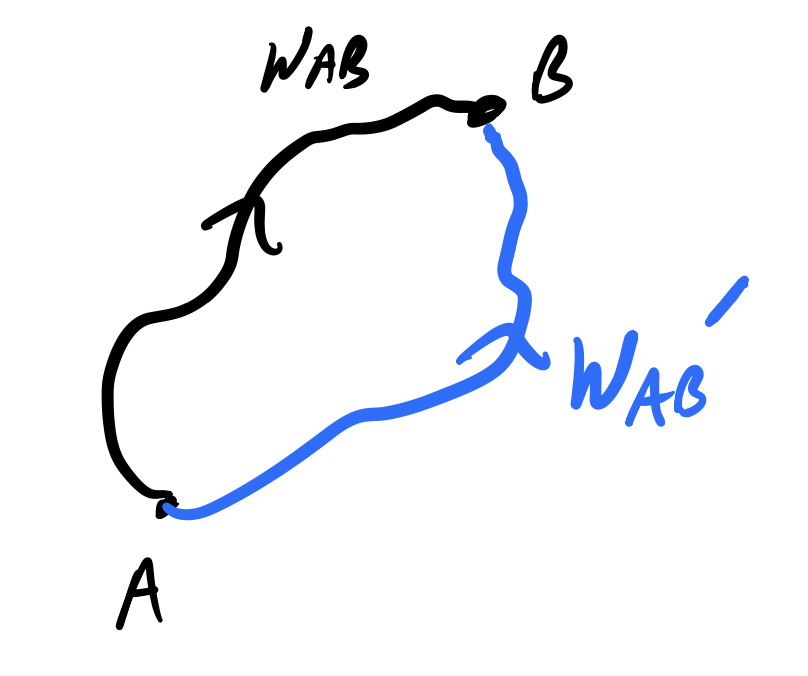
\includegraphics[scale=0.3]{Lectures/Images/lec2-work.png}
\end{center}
In this case, we have net work (positive or negative, depending on the sign) when we go around a cycle. The work done is rate-independent (no time derivatives here!). Further, the medium must be chiral because there is a difference in the sign of work depending on whether we traverse a loop clockwise or counterclockwise.

\subsection{Representations of Stress/Strain Tensors}
Let's try to classify all possibel entries of the stiffness tensor $K_{ijkl}$ using the representations of $\sigma$ and $u$; this will allow us to classify possible elastic moduli. In particular, let us try to classify odd elasticity $K^o_{ijkl}$ in 2-dimensions. In 2-D, stress $\sigma_{ij}$ and strain $u_{kl}$ each have 4-independent components, which we may package into a 4-entry vector. Therein the stiffness $K_{\alpha\beta}$ is a 4x4 matrix that connects them. We ``play God'' by analyzing/studying the form of $K_{\alpha\beta}$ without knowing any details about our system - we can deduce constraints purely mathematically.

\begin{center}
    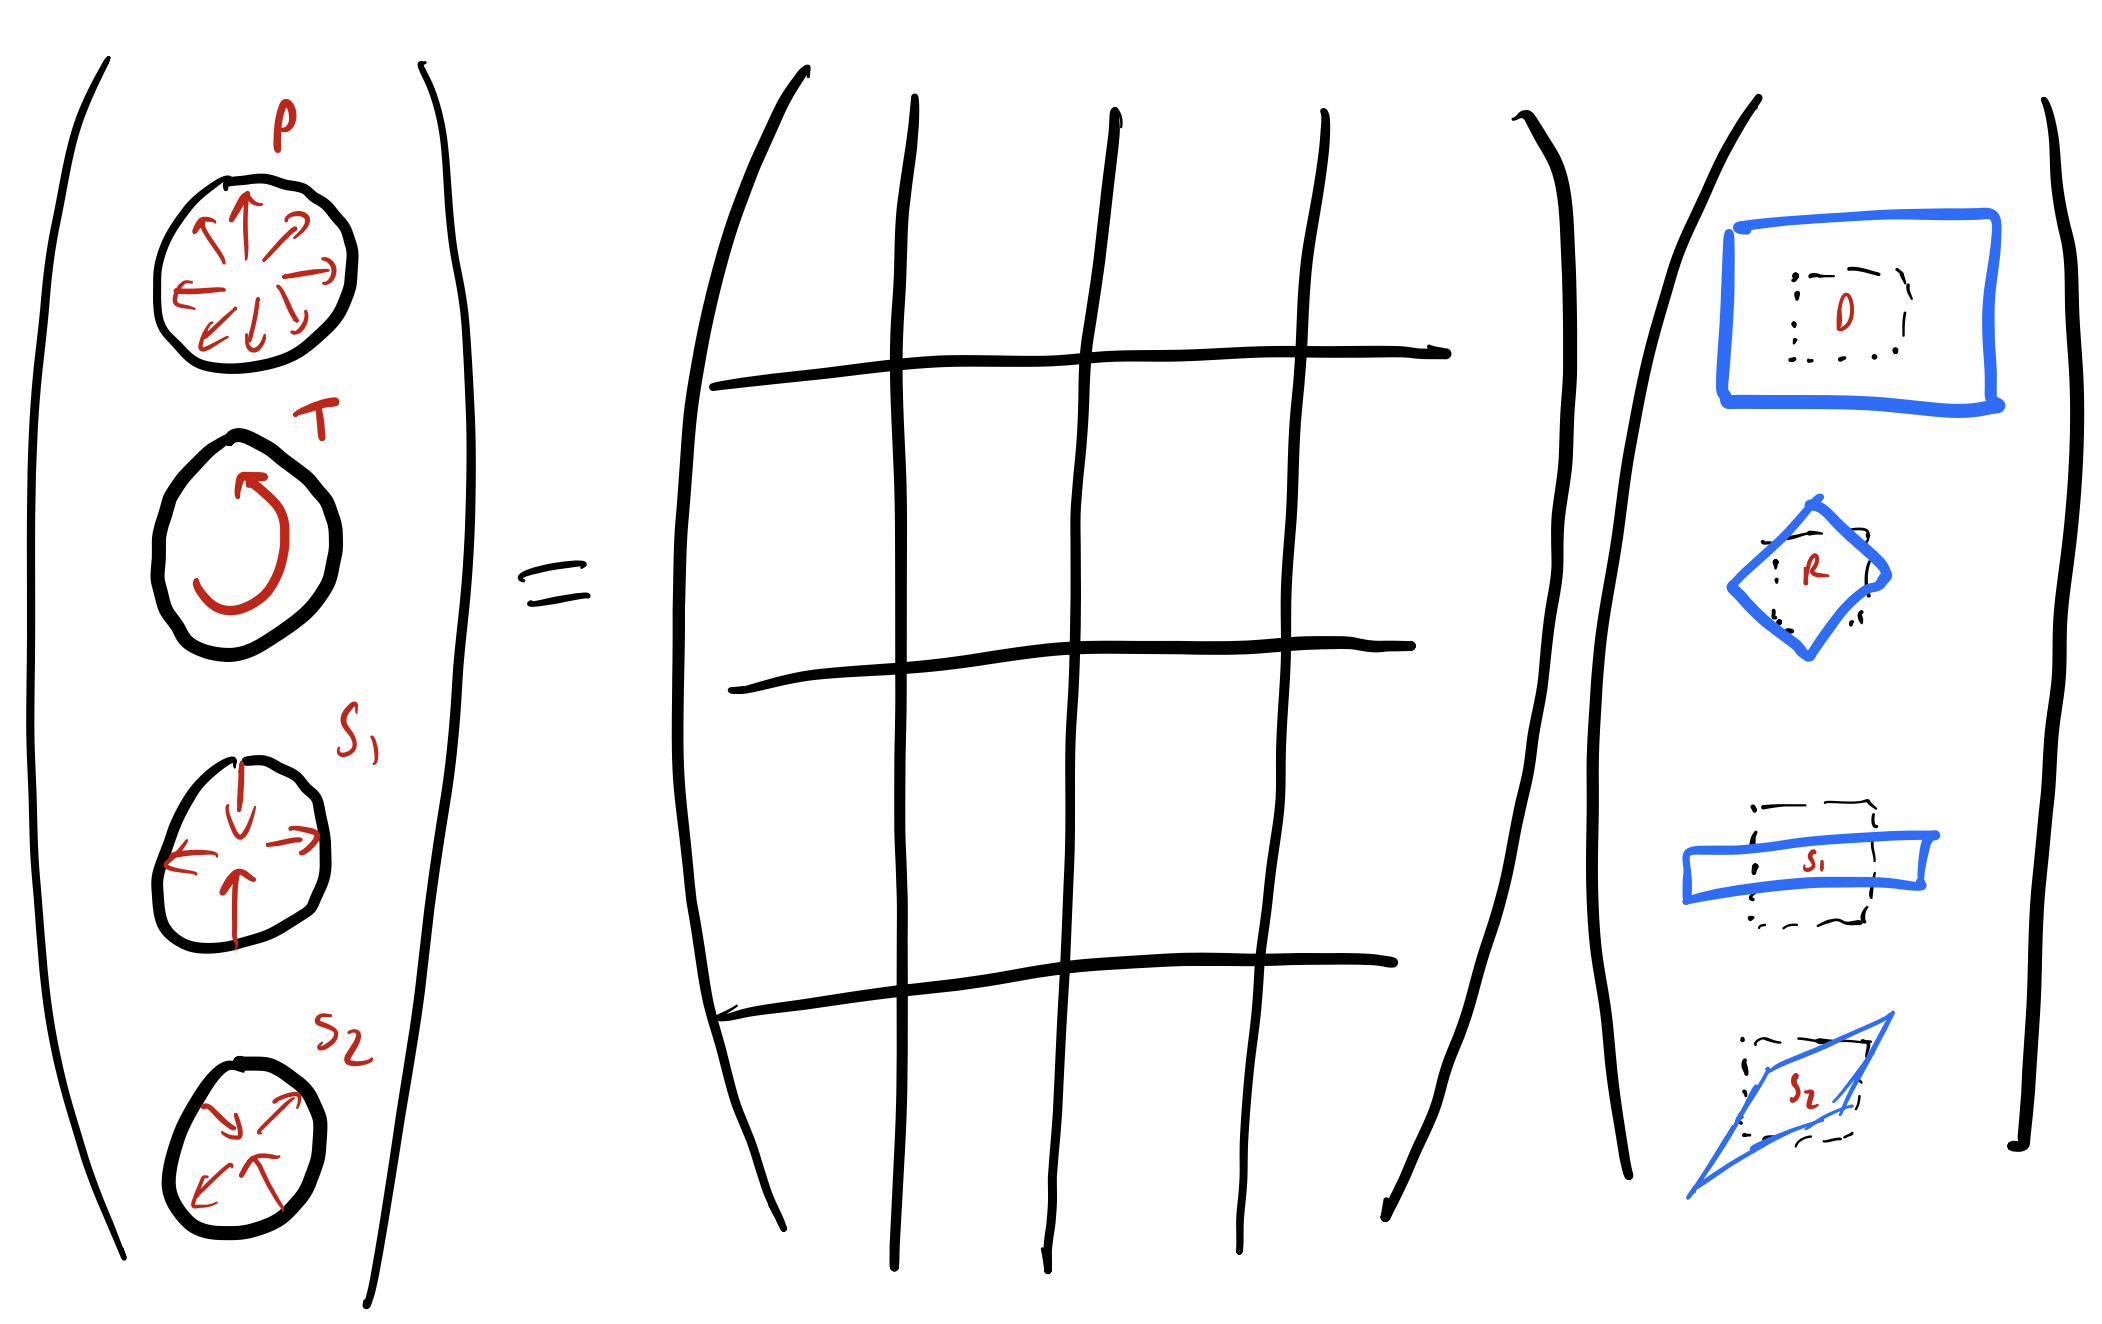
\includegraphics[scale=0.35]{Lectures/Images/lec2-stiffnessmatrix.png}
\end{center}
\begin{equation}
    \m{\text{P} \\ \text{T} \\ \text{SS1} \\ \text{SS2}} = \m{\cdot & \cdot & \cdot & \cdot \\ \cdot & \cdot & \cdot & \cdot \\ \cdot & \cdot & \cdot & \cdot \\ \cdot & \cdot & \cdot & \cdot}\m{\text{D} \\ \text{R} \\ \text{S1} \\ \text{S2}}
\end{equation}

The four entries of strain $u_{\beta}$ will be the projections onto the basis elements of dilation, rotation, 2 shears. We can do the same for stress, writing down the forces that result from the deformations - pressure, torque, and shear stress 1/2. Then the matrix elements of $K_{\alpha\beta}$ relate the two.

What is the analytical meaning of the drawings above? We write:
\begin{equation}
    u_{ij} = \sum_{\alpha=0}^3 u^\alpha \tau_{ij}^\alpha
\end{equation}
with:
\begin{equation}
    \tau^0 = \m{1 & 0 \\ 0 & 1}, \quad \tau^1 = \m{0 & 1 \\ -1 & 0}, \quad \tau^2 = \m{1 & 0 \\ 0 & -1}, \quad \tau^3 = \m{0 & 1 \\ 0 & 1}
\end{equation}
Corresponding to dilation, rotation, shear 1, and shear 2 respectively. Note that these obey the relation (note that we take a trace below, since the indices are repeated and hence summed):
\begin{equation}
    \boxed{\tau_{ij}^\alpha \tau_{ij}^\gamma = 2\delta^{\alpha\gamma}}
\end{equation}
This is the algebra for the generators of the rotation group in 2-D.

This was a statement about the geometry of the strain deformation. We can do a similar procedure for the stress:
\begin{equation}
    \sigma_{ij} = \sum_{\alpha=0}^3 \sigma^\alpha \tau^\alpha_{ij}
\end{equation}
where now the projections onto $\tau^0, \tau^1, \tau^2, \tau^3$  correspond to pressure, torque, shear stress 1, shear stress 2.

\subsection{Classifying elastic moduli}
Now, we want to discover what is in the $K_{\alpha\beta}$ matrix. To this end, we can think about symmetries of the medium. One such symmetry/idea is isotropy - wherein there is no preferred direction to the material. With this assumption we can already set a lot of the entries of $K$ to zero. 

In a world that is isotropic, I cannot couple a scalar/pseudoscalars to a vector/bivectrs - why? Because this would involve a preferred direction. So, look at the matrix element of $K$ that connects dilation with shear stress. We cannot measure the angle of shear in a isotropic medium, so this matrix element must vanish.

More generally, the dilation/rotation subspaces are scalar/pseudoscalars, and the stress subspaces are pseudovectors. Further, pressure/torque are scalar/pseudoscale and shear stress are pseudovector. By isotropy the subspaces cannot be connected, which allows us to conclude that 8 of the entries vanish:

\begin{equation}
    \m{\text{P} \\ \text{T} \\ \text{SS1} \\ \text{SS2}} = \m{\cdot & \cdot & 0 & 0 \\ \cdot & \cdot & 0 & 0 \\ 0 & 0 & \cdot & \cdot \\ 0 & 0 & \cdot & \cdot}\m{\text{D} \\ \text{R} \\ \text{S1} \\ \text{S2}}
\end{equation}

Next, consider the symmetry of objectivity/frame invariance. We can consider the solid to be ``self-standing'' - in this case, applying a rigid body rotation applies no stress. Note that we can break this if the solid was standing on some sticky surface (in which case we could have stresses applied from the contact) - symmetries can be broken by perturbations, e.g. isotropy via a magnetic field. But what does this frame invariance give us for the stiffness tensor? Since rotation generates no stresses, the entire second column is set to zero (rotations cannot generate pressure or torques).

\begin{equation}
    \m{\text{P} \\ \text{T} \\ \text{SS1} \\ \text{SS2}} = \m{\cdot & 0 & 0 & 0 \\ \cdot & 0 & 0 & 0 \\ 0 & 0 & \cdot & \cdot \\ 0 & 0 & \cdot & \cdot}\m{\text{D} \\ \text{R} \\ \text{S1} \\ \text{S2}}
\end{equation}

We have assumed that linear momentum is conserved. We have not used energy conservation here - let's see what this implies for us now.

To learn about the last remaining entries, let us work through some algebra. We write:
\begin{equation}
    \sigma_{ij} = \textcolor{blue}{\sigma^\gamma \tau^\gamma_{ij}} = K_{ijkl} = u_{kl} = \textcolor{blue}{K_{ijkl}\tau^\beta_{kl}u^\beta}
\end{equation}
Now multiplying the blue by $\frac{1}{2}\tau^\alpha_{ij}$, then on the LHS I get:
\begin{equation}
    \frac{1}{2}\tau^\alpha_{ij}\sigma^\gamma \tau^\gamma_{ij} = \frac{1}{2}\sigma^\gamma 2\delta^{\alpha\gamma} = \sigma^\alpha
\end{equation}
and on the RHS we get:
\begin{equation}
    \frac{1}{2}\tau^\alpha_{ij} K_{ijkl}\tau^\beta_{kl}u^\beta
\end{equation}
so:
\begin{equation}
    \sigma^\alpha = \frac{1}{2}\tau^\alpha_{ij} K_{ijkl}\tau^\beta_{kl}u^\beta = K^{\alpha\beta}u^\beta
\end{equation}
So, if we assume that the theory is conservative/we have reciprocity $K_{ijkl} = K_{klij}$, then $K^{\alpha\beta} = K^{\beta\alpha}$ - the matrix is symmetric, and so we can set the matrix element that connects dilation to torque is zero:
\begin{equation}
    \m{\text{P} \\ \text{T} \\ \text{SS1} \\ \text{SS2}} = \m{\cdot & 0 & 0 & 0 \\ 0 & 0 & 0 & 0 \\ 0 & 0 & \cdot & \cdot \\ 0 & 0 & \cdot & \cdot}\m{\text{D} \\ \text{R} \\ \text{S1} \\ \text{S2}}
\end{equation}
We can name some of the remaining entries; the entry connecting dilation to pressure is the bulk modulus $B$:
\begin{equation}
    \m{\text{P} \\ \text{T} \\ \text{SS1} \\ \text{SS2}} = \m{B & 0 & 0 & 0 \\ 0 & 0 & 0 & 0 \\ 0 & 0 & \cdot & \cdot \\ 0 & 0 & \cdot & \cdot}\m{\text{D} \\ \text{R} \\ \text{S1} \\ \text{S2}}
\end{equation}
Now, it is an exercise that you may have on a problem set that isotropy constrains the lower diagonal entries to be the same, and the lower off-diagonal entries to be equal and opposite. The diagonals we can call the shear modulus $G$, and the off-diagonals must be zero (as energy conservation constrains $K^{\alpha\beta}$ to be symmetric). Thus:
\begin{equation}
    \m{\text{P} \\ \text{T} \\ \text{SS1} \\ \text{SS2}} = \m{B & 0 & 0 & 0 \\ 0 & 0 & 0 & 0 \\ 0 & 0 & G & 0 \\ 0 & 0 & 0 & G}\m{\text{D} \\ \text{R} \\ \text{S1} \\ \text{S2}}
\end{equation}

So, if we assume isotropy, frame invariance, and conservative forces, we just have $B, G$ above. Let's repeat the analysis if we do not assume conservative forces. The diagonal components are not affected, but the off-diagonal entries we constrained to be zero are now generically nonzero:
\begin{equation}
    \m{\text{P} \\ \text{T} \\ \text{SS1} \\ \text{SS2}} = \m{B & 0 & 0 & 0 \\ A & 0 & 0 & 0 \\ 0 & 0 & G & -K^0 \\ 0 & 0 & +K^0 & G}\m{\text{D} \\ \text{R} \\ \text{S1} \\ \text{S2}}
\end{equation}

So, this is the conclusion of our analysis - we have (relaxing energy conservation) 4 moduli describing our material. 

Comment: In an anisotropic medium, we could have the moduli coupling the two shears, but they will \emph{not} be equal and opposite. One could then imagine matrix elements of the form $\e + K^0, \e - K^0$; one must look at the \emph{difference} to conclude nonconservative forces (just looking at one element, you cannot be sure if the source is anisotropy). Additionally, a nonzero $A$ does not necessarily mean nonconservative forces, it means nonconservative forces \emph{and} frame invariance, so to conclude nonconservative forces concretely we would need to compare with the other matrix element across the diagonal.

\subsection{Quantifying Work}
We derive the expression for the work coming from the stresses. For a force we have the contour integral:
\begin{equation}
    W = -\oint \v{F} \cdot d\v{l}
\end{equation}
For stresses, we consider a loop integral in 4-D space:
\begin{equation}
    W = -\oint \sigma_{ij}du_{ij} = -\oint \sigma^\beta du^\beta
\end{equation}
Now using Stokes' theorem:
\begin{equation}
    W = \iint \e^{\alpha\beta}\frac{\partial \sigma^\beta}{\partial u^\alpha}dA
\end{equation}
With $\e^{\alpha\beta} = \m{0 & -1 \\ 1 & 0}$. Now, we can use that $\sigma^\beta = K^{\beta\alpha}u^\alpha$, and take the derivative. Note that we can focus solely on the entries of the tensor coming from the non-conservative forces (the parts coming from conservative forces give trivially zero contribution)! Writing $K^{\alpha\beta} = K^0e^{\alpha\beta}$ (we focus on the subspace of shears), we get:
\begin{equation}
    W = -\iint \e^{\alpha\beta}e^{\beta\alpha}K^0 dA
\end{equation}
Then:
\begin{equation}
    \e^2 = \m{-1 & 0 \\ 0 & -1} \implies -\e^{\alpha\beta}e^{\beta\alpha} = 2
\end{equation}
and so:
\begin{equation}
    W = 2K^0 \cdot \text{Area}
\end{equation}
So we see that we do indeed have a nonzero amount of work, proportional to the odd elastic modulus and enclosed area.
\section{Microscopic Sources of Exotic Stiffness}

\subsection{Review}
Last time, we tried to constrain the stiffness tensor:
\begin{equation}
    \sigma^\alpha = K^{\alpha\beta}u^\beta
\end{equation}

Assuming isotropy, the subspaces of scalars and vectors could not be connected (so the off diagonal blocks vanish), and assuming frame invariance, rotations cannot generate any stresses, so:
\begin{equation}
    \m{\text{P} \\ \text{T} \\ \text{SS1} \\ \text{SS2}} = \m{\cdot & 0 & 0 & 0 \\ \cdot & 0 & 0 & 0 \\ 0 & 0 & \cdot & \cdot \\ 0 & 0 & \cdot & \cdot}\m{\text{D} \\ \text{R} \\ \text{S1} \\ \text{S2}}
\end{equation}
Isotropy further contains that the lower diagonals are the same and lower off diagonals are the same, so the most general form of the tensor is:
\begin{equation}\label{eq:macroscopic}
    \m{\text{P} \\ \text{T} \\ \text{SS1} \\ \text{SS2}} = \m{B & 0 & 0 & 0 \\ A & 0 & 0 & 0 \\ 0 & 0 & G & -K^0 \\ 0 & 0 & +K^0 & G}\m{\text{D} \\ \text{R} \\ \text{S1} \\ \text{S2}}
\end{equation}
Important point - the existence of the odd elastic moduli $K^0$ implies two things. First, the structure of the theory is non-variational; we can go around quasi-statically in the space of strains, and we find the work is nonzero:
\begin{equation}
    W = \oint \sigma_{ij}du_{ij}\neq 0
\end{equation}
This tells us that there is a chirality in the material (this was also manifest from the fact that - if $G = 0$, then the part of the stiffness matrix acting on the shear subspace looks like $K^0\e$). Another clear manifestation of chirality is if $A \neq 0$, in which case we can have torques (note - no angular momentum conservation!) as a result of dilations.

\subsection{Non-reciprocal gadget and constructions}
This is an example of a $K^0 \neq 0, A = 0$ system from a recent Nature paper \texttt{Veenstra, Scheibner, Brandenbourger, Binysh, Souslov, Vitelli, Coulais. \emph{Nature} (2025)}. As warm-up, consider the following spring system:

\begin{center}
    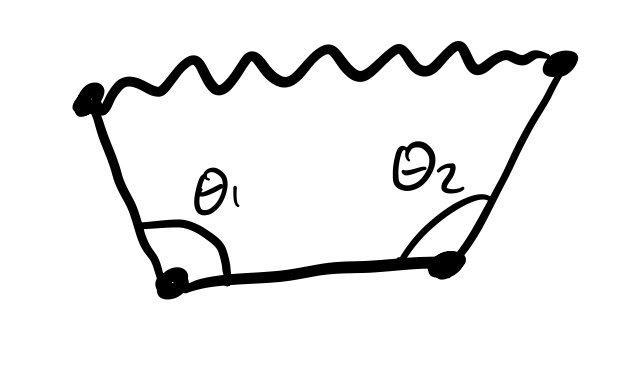
\includegraphics[scale=0.35]{Lectures/Images/lec3-gadgetwithspring.png}
\end{center}

If we have a bond-bending interaction, we have a bond-bending stiffness:
\begin{equation}
    \m{\tau_1 \\ \tau_2} = \m{-\kappa & \kappa^s \\ \kappa^s & -\kappa}\m{\delta\theta_1 \\ \delta\theta_2}
\end{equation}
where the diagonals come from the bond-bending, and the off-diagonals (symmetric!) come from the coupling spring. For this system:
\begin{equation}
    \nabla \times \gv{\tau} = \v{0}
\end{equation}
but we can introduce batteries/motors to break this symmetry. If Maxwell-Betti reciprocity is obeyed, then pushing one side of the object should repel the other symmetrically. But we can introduce motors to make this building block non-reciprocal; pressing on the left side the right side repels, pressing on the right side the left side \emph{attracts}.
\begin{center}
    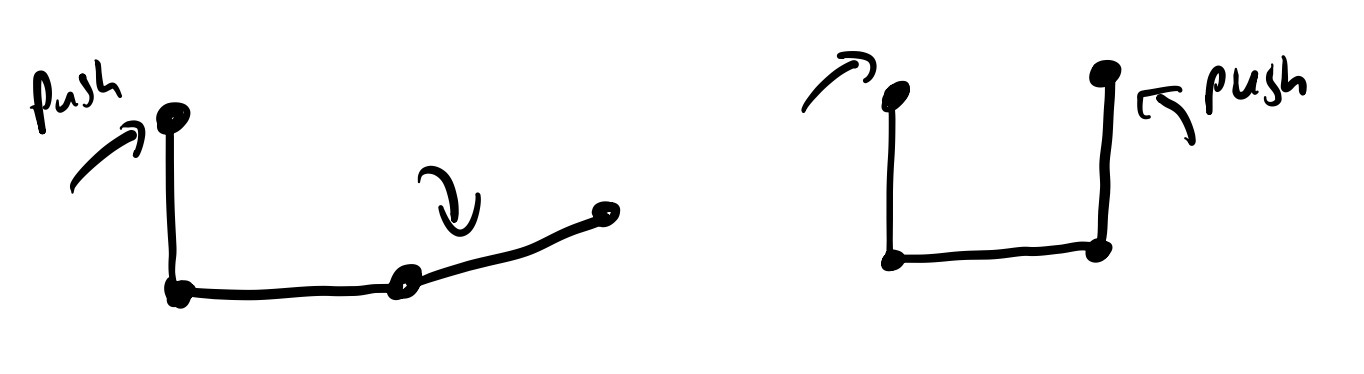
\includegraphics[scale=0.35]{Lectures/Images/lec3-nonreciprocalgadget.png}
\end{center}
This means that we have a stiffness tensor of the form:
\begin{equation}\label{eq:microscopic}
    \m{\tau_1 \\ \tau_2} = \m{-\kappa & -\kappa^a \\ \kappa^a & -\kappa}\m{\delta\theta_1 \\ \delta\theta_2}
\end{equation}

A technical comment - notice that the interaction we've written above is a striking example of a non-pairwise interaction. The torque at point 1 doesn't just depend on the pair of rods eminating out of it, but also from the other components of the system.

What is the physical consequence of this non-reciprocal interaction? Now, we can go through a cycle and generate non-zero work. If we make a ring of these objects - with the motors off, the system jiggles a bit before being slowed to rest with friction. With the motors on, we perturb the medium and in trying to undo the deformation/get back to the starting point the motors can induce energies into the system and the system can keep jiggling forever (using the energy provided by the external motors).

If we think about the dynamics, we have:
\begin{equation}
    \m{I\delta \ddot{\theta}_1 \\ I\delta \ddot{\theta}_2} = \m{-\kappa & -\kappa^a \\ \kappa^a & \kappa}\m{\delta \theta_1 \\ \delta\theta_2}
\end{equation}
If we diagonalize to find the normal frequencies, we have:
\begin{equation}
    \omega^2 = \frac{\kappa}{I} \pm i\frac{\kappa^a}{I}
\end{equation}
The first term makes total sense - this is what we have for just a regular spring system that you've seen many times before in classical mechanics. But the antisymmetric term produces an imaginary component to $\omega^2$! This means that (in the absence of nonlinearities - we have assumed linear response for this whole discussion) we have unbounded growth/amplification of the motion! Of course building this gadget in real life we do in fact have nonlinearities - when the angles become large the components of the gadget can touch - which prevents unbounded growth.

Now, we can take our object - where the antisymmetric $\kappa^a$ breaks the chiral symmetry - and map out the dynamics in strain space (with the two shears being the two axes). The system can exhibit chaotic behaviour!

Let us ``rediscover'' the wheel (again, still composed of the the gadget). Original conception of a wheel has a circular, fixed shape which moves via force supplied to it from axle (via animal, motor etc.) But our new wheel is adaptive, and moves via deformations. It can come across a rough uphill landscape and use the deformations caused by the rough landscape to travel through it! In fact we can make the problem even harder - we can make a landscape of granular uphill matter, and our sophisticated wheel can still go up it (we can also flip the sign of $\kappa^a$ - we are allowed to pick/tune whatever sign for these - and it can travel the other way).

We can also build up a crystal out of this gadget by tiling. We can throw a projectile onto the crystal, which is then ejected back upwards at an angle (the angle/asymmetric response is expected! The medium is chiral. Again, we can flip the angle by flipping the sign of $\kappa^a$).

Motivating a homework problem you will do - there is a microscopic law Eq. \eqref{eq:microscopic} and the macroscopic/continuum description Eq. \eqref{eq:macroscopic}. Without calculation, we can deduce $K^0 \sim \kappa^a$ and $G \sim \kappa$. We can do a more detailed derivation and derive the macroscopic dependence on the microscopic parameters (and then check that this dependence works out in experiment)! In your homework, you will just take a normal (not odd!) hexagonal microscopic lattice, and see how the macroscopic properties/parameters and their dependencies emerge.

\subsection{Microscopic source of $A$}

If we have a central force, we can generically write things as a gradient of a potential. We introduce non-conservative forces in terms of a non-central part. Consider the spring:

\begin{center}
    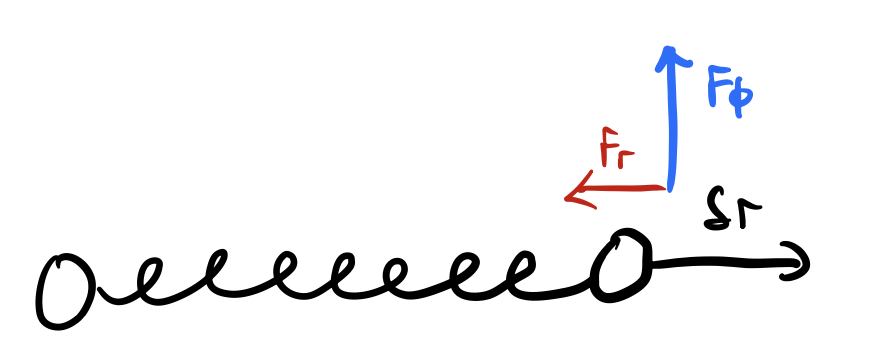
\includegraphics[scale=0.35]{Lectures/Images/lec3-noncentralspring.png}
\end{center}

\begin{equation}
    \v{F} = -(\kappa\hat{\v{r}} + \kappa^a\hat{\gv{\phi}})\delta r
\end{equation}
Or as a matrix equation:
\begin{equation}
    \m{F_r \\ F_\phi} = \m{-\kappa & 0 \\ -\kappa^a & 0}
\end{equation}
Notice again the crucial point - the off-diagonals are \emph{not} equal. This implies that:
\begin{equation}
    \oint \v{F} \cdot d\v{l} \propto \kappa^a
\end{equation}
(and does not vanish). The central part does not contribute to the net work as to the central part we can always prescribe a potential. Generally here, $\v{F} \neq -\nabla U$ so long as $\kappa^a \neq 0$. If we built up a lattice/continuum out of this microscopic piece, we could derive how the $A$ modulus emerges from the nonzero $\kappa^a$.

Let us consider a simple exercise - let's derive the work done in a cycle.

\begin{center}
    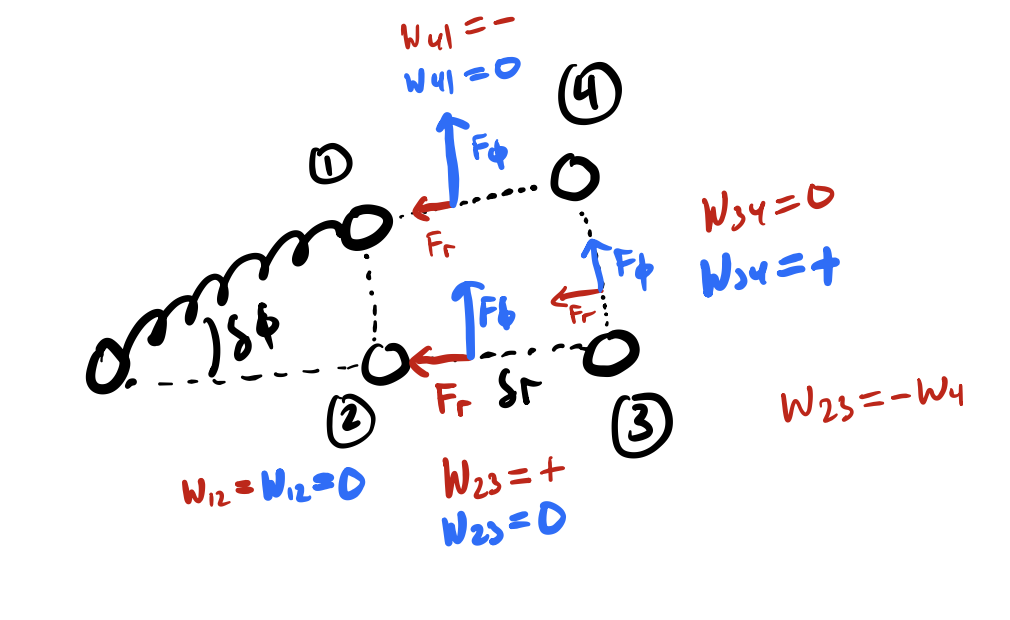
\includegraphics[scale=0.5]{Lectures/Images/lec3-noncentralspringwork.png}
\end{center}

\begin{itemize}
    \item From 1 to 2, there is no force and hence no work done.
    \item From 2 to 3, the direction of motion is radial, so only the radial component of the force contributes (positive) work.
    \item From 3 to 4, the direction of motion is tangential, so the tangential component of the force picks up (positive) work.
    \item From 4 to 1, the direction of motion is radial, so the radial component of the force contributes (negative) work. This work is equal and opposite to the work in step 2$\to$3.
\end{itemize}

Thus only surviving term is $W_{34}$ arising from $F_\phi$, which we can calculate to be:
\begin{equation}
    \oint \v{F} \cdot d\v{l} = W_{34} = F_\phi dl = \kappa^a \delta r (r + \delta r)\delta \phi \approx \kappa^a (r\delta \phi)\delta r = \kappa^a \cdot \text{Area}
\end{equation}

So in the harmonic approximation, with:
\begin{equation}
    F''(r) = F''(a) - \kappa(r - a), \quad F_\perp \approx F^\perp(a) - \kappa^a(r - a)
\end{equation}
we can derive the bulk and shear moduli:
\begin{equation}
    B = \frac{\sqrt{3}}{2}\left(\kappa + \frac{F''(a)}{a}\right), \quad G = \frac{\sqrt{3}}{4}\left(\kappa - 3\frac{F''(a)}{a}\right)
\end{equation}
as well as the $K^0/A$ moduli:
\begin{equation}
    A = -\frac{\sqrt{3}}{2}\left(\kappa^a - \frac{F^\perp(a)}{a}\right), \quad K^0 = \frac{\sqrt{3}}{4}\left(\kappa^a - 3\frac{F^\perp(a)}{a}\right)
\end{equation}
note that the precise dependence depends on not just the force mechanism but also the layout of the lattice (e.g. will change with hexagonal, square etc.). If we did a similar derivation with the non-reciprocal robot gadget, we could also derive a macro-from-micro result from above (see the paper!), with $A = 0$ and $K^0 \neq 0$.

\subsection{Other contemporary experiments}

There have been a number of recent experiments that measure interesting non-central crystals. For example colloidal spinners in a magnetic field that form odd elastic crystals \texttt{Bililign, Usabiaga, Ganan, Poncet, Soni, Magkiriadou, Shelley, Bartolo, Irvine. \emph{Nature} (2022)} or crystal formation in biological platforms \texttt{Tan, Mietke, Higinbotha, Li, Chen, Foster, Gokhale, Dunkel, Fakhri. \emph{Nature} (2022)}.

In such non-central crystals, there is the potential to measure lubrication forces:

\begin{center}
    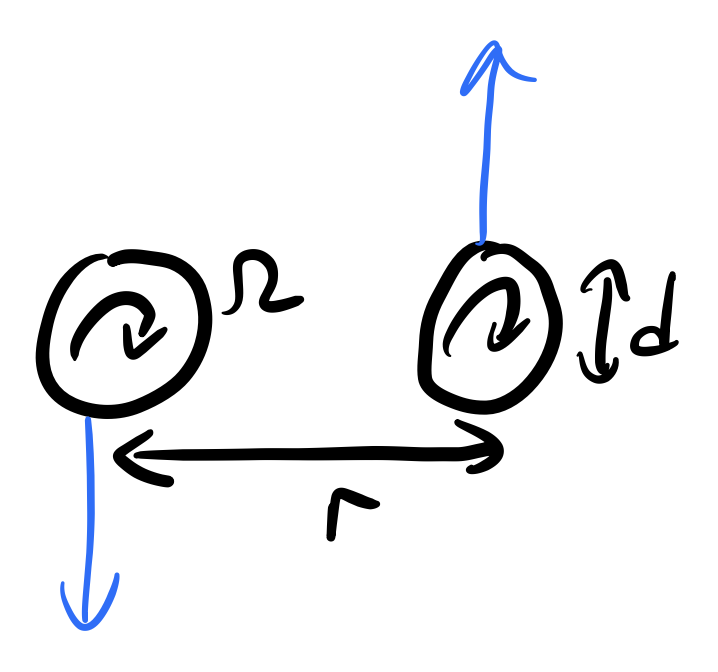
\includegraphics[scale=0.35]{Lectures/Images/lec3-lubricationforces.png}
\end{center}

where:
\begin{equation}
    F^\perp \propto \Omega \log\left(\frac{r - d}{d}\right)
\end{equation}

Next time - we will take the macroscopic theory, and study the stability of the lattice, as well as excitations (sound modes) in it. These have been concretely measured in robotic platform, and allegedly in the biological platform above (and perhaps possible to measure it in the colloidal spinner crystal?) however in the latter two cases the micro-to-macro correspondence is much well less understood.
\section{Odd Elastodynamics}

Last time, we looked at microscopic models where odd elasticity could arise. We also looked in detail at how energy could be generated in cycles of such system. Today we look odd elastodynamics, and study the dynamical equation for the displacement field. The presentation will be more algebraic.

In the last few lectures, we had pictures of different stresses/strains - these were pictorial representations of tensors, and in this lecture we make a dictionary to map between the pictures and algebra. For example we'll see how the tensors:
\begin{equation}
    \m{1 & 0 \\ 0 & 1} \to \delta_{ij}, \quad \m{0 & -1 \\ 1 & 0} \to \e_{ij}
\end{equation}
connect to stress/strain. For simplicity, we stay in 2D.

We recall the stress/strain relation:
\begin{equation}
    \sigma_{ij} = K_{ijmn}\p_m u_n  = K_{ijmn}u_{mn}
\end{equation}
Where we have the stiffness tensor $K_{ijmn}$. We wrote this relation (using symmetry constraints) as:
\begin{equation}\label{eq:macroscopic}
    \m{\text{P} \\ \text{T} \\ \text{SS1} \\ \text{SS2}} = \m{B & 0 & 0 & 0 \\ A & 0 & 0 & 0 \\ 0 & 0 & G & -K^0 \\ 0 & 0 & +K^0 & G}\m{\text{D} \\ \text{R} \\ \text{S1} \\ \text{S2}}
\end{equation}
Note that if $\sigma_{ij} = \frac{\delta \e}{\delta u_{ij}}$, then $K_{ijmn} = K_{mnij}$, but if $\sigma_{ij}$ is not of this form then $K$ is not necessary symmetric, so we can have the elastic moduli $K^0, A$ emerge in the stiffness tensor.

\subsection{Algebraic Representation of Stiffness Tensor}
Let's now switch to an algebraic representation:
\begin{equation}
    K_{ijmn} = B\delta_{ij}\delta_{mn} - A\e_{ij}\delta_{mn} + G(\delta_{in}\delta_{jm} + \delta_{im}\delta_{jn} - \delta_{ij}\delta_{mn}) + K^0 \frac{1}{2}(\e_{im}\delta_{jn} + \e_{in}\delta_{jm} + \e_{jm}\delta_{in} + \e_{jn}\delta_{im})
\end{equation}
The first term corresponds to the bulk modulus, which connects the dilation (projection of $u_{mn}$ onto identity/$\delta_{mn}$) and the pressure (projection of $\sigma_{ij}$ onto identity/$\delta_{ij}$). Thus it is not surprising that it has the form above; explicitly, they are derived via:
\begin{equation}
    P\delta_{ij} = B(\nabla \cdot \v{u})\delta_{ij} \implies \sigma_{ij} = \left[B\delta_{ij}\delta_{mn}\right]\p_m u_n
\end{equation}
For torque, we project $\sigma_{ij}$ onto the antisymmetric matrix $\e_{ij}$ (the sign of $A$ in $K_{ijmn}$ is up to convention of dilation - we choose it to be negative so we get a positive sign in the equation of motion):
\begin{equation}
    T\e_{ij} = A(\nabla \cdot \v{u})\e_{ij} \implies \sigma_{ij} = \left[A\e_{ij}\delta_{mn}\right]\p_m u_n
\end{equation}

Note that the $G$ term is invariant/same sign (even) under $ij \leftrightarrow mn$, while the $K^0$ term flips sign (odd) under $ij \leftrightarrow mn$.

\subsection{Equation of Motion}
I can now calculate the stress in terms of the strain, and taking one more derivative of the stress I can get the force. Then we obtain the equation of motion for odd elasticity!

\begin{equation}
    \rho \p_t^2 u_j + \Gamma \p_t u_j = F_j = \p_i \sigma_{ji} = \p_i (K_{jimn} \p_m u_n ) = K_{jimn}\p_i \p_m u_n
\end{equation}
where we note that the $\p_i$ commutes across the $K_{jimn}$ as the stiffness tensor is position independent (just a tensor of numbers). Thus, we have an EoM that relates a first + second time derivative to a second spatial derivative of displacement/strain.

If we looked at the robots of last time (centimeter scale), the first/inertial term $\rho \p_t^2 u_j$ is important. But for very small systems we can consider the overdamped limit (equivalently - the low Reynolds number\footnote{$R = \frac{uL}{\nu}$ with $u$ the velocity, $L$ the characteristic size, $\nu$ the viscosity} limit):
\begin{equation}
    \Gamma \dot{u}_j \gg \rho \ddot{u}_j.
\end{equation}
Thus, in the analysis of our equations of motion we neglect the inertial term.

A good exercise is to massage the derivatives until the terms with two spatial derivatives have recognizable form. For the $B$ term, we get:
\begin{equation}
    \Gamma \p_t u_j = \p_i K_{jimn} \stackrel{B-term}{=} \p_i B \delta_{ji}\delta_{mn}u_{mn} = B\p_j \p_i u_i
\end{equation}
or as a vector:
\begin{equation}
    \Gamma \p_t \v{u} = B\nabla(\nabla \cdot \v{u})
\end{equation}
For the $A$ term, we get:
\begin{equation}
    \Gamma \p_t u_j = \p_i K_{jimn} \stackrel{A-term}{=} A\e_{ji}\delta_{mn}\p_i u_{mn} = A\e_{jk}\p_k \p_i u_i
\end{equation}
or as a vector:
\begin{equation}
    \Gamma \p_t \v{u} = A\zhat \times \nabla(\nabla \cdot \v{u})
\end{equation}

Writing down the other terms:
\begin{equation}
    \Gamma \p_t u_j = B\nabla(\nabla \cdot \v{u}) + G\nabla^2u_j + A\e_{jk}\p_k \p_i u_i + K^0\e_{jk}\nabla^2 u_k 
\end{equation}
or vectorially:
\begin{equation}
    \Gamma \p_t \v{u} =B\nabla(\nabla \cdot \v{u}) + G\nabla^2\v{u} + A\zhat \times \nabla(\nabla \cdot \v{u}) + K^0 \zhat \times (\nabla^2 \v{u})
\end{equation}

\subsection{Limits and Physical Interpretations}
Note that if $B = A = K^0 = 0$, then we just have a diffusion equation. So one interpretation of what we have derived is a non-reciprocal diffusion equation.

Note that if instead we worked in the underdamped limit, we would have:
\begin{equation}
    \rho \p_t^2 \v{u} = G\nabla^2 \v{u}
\end{equation}
which is a wave equation, with wave speed $c = \sqrt{\frac{G}{\rho}}$. This wave equation is predicated on two things - that we have a nonzero shear modulus and that we have a second derivative in time. If we kill the second derivative, we overdamp the oscillations. If we work in a medium with $B \approx G \approx 0$, so the medium is not elastic/we've killed the ability of the medium to rattle kinetic energy to potential energy (you can interpret $B/G$ as the spring constants of your medium). 

Now the question is - can we be in the overdamped regime and in the regime where $K^0 \gg G, B, A$ and have the medium still support waves? The answer is, strikingly, yes! We'll watch a movie next time, but for now let's write down the equation in this limit:
\begin{equation}
    \Gamma\m{\dot{u}_x\\\dot{u}_y} = \m{0 & -K^0 \\ K^0 & 0}\nabla^2\m{u_x \\ u_y}
\end{equation}
If we did not throw away the shear modulus $G$, then we would have diagonal components and diffusion transport. But in this limit we still have the interesting cross-diffusion terms. This might remind us of Hamilton's equation for the harmonic oscillator, where for $U = \frac{1}{2}x^2$ ($m=k=1$):
\begin{equation}
    \dot{x} = p, \dot{p} = -\p_x U \implies \p_t\m{x \\ p} = \m{0 & 1 \\ -1 & 0}\m{x \\ p}
\end{equation}
We note the symplectic matrix:
\begin{equation}
    \Omega = \m{0 & 1 \\ -1 & 0}
\end{equation}
which is what is responsible for the oscillatory behavior (the fact that they are conjugate coordinates is what further gives us energy conservation). Here $u_x, u_y$ are not canonical conjugate coordinates, but seeing that it has the same symplectic structure, we will have oscillatory behaviour (you might object that we have the Laplacian $\nabla^2$ - but we can get rid of this via Fourier transform, so the Laplacian just gives a $k^2$). Interestingly, the shear modulus $G$ actually hinders the elasticity, while the odd elasticity $K^0$ is responsible for the wave propagation.

Formally, we can write solutions:
\begin{equation}
    u_i(\v{x}) = \tilde{u}_i(\v{q})e^{i(\v{q} \cdot \v{x} - \omega t)}
\end{equation}
where:
\begin{equation}
    \omega = \frac{K^0}{\Gamma}q^2
\end{equation}
Ok, so we get oscillatory behaviour. But why? The intuition is the following - work is no longer a state function, so if we have cycles, we can take in or put out energy in a rate-independent manner. So, if we have an odd elastic medium, we peturb it, then the medium can go through a cyclic deformation, wherein it can take in energy to keep the motion going (rather than dissipating it).
\section{Odd Elastodynamics II}

\subsection{Review of Last Lecture}
We wrote down an equation of motion for the displacement field:
\begin{equation}
    \overbrace{\rho \p_t^2 u_j}^{\text{inertia}} + \overbrace{\Gamma \p_t u_j}^{\text{drag}} = B\p_j \p_i u_i + G \nabla^2 u_j + A\e_{jk}\p_k \p_i u_i + K^0\e_{jk}\nabla^2 u_k
\end{equation}
what we keep on the LHS depend on whether we work in the overdamped/underdamped limit. What is present on the RHS depends on the terms that appear in the constitutive equation $\sigma_{ij} = K_{ijmn}u_{mn}$. $B$ is the bulk modulus, $G$ is the shear modulus, $A, K^0$ are the odd moduli - $A$ couples to the antisymmetric part of the stress tensor and gives rise to torque. $K^0$ relates to the shears, and can arise even if $\sigma_{ij} = \sigma_{ji}$.

We consider the overdamped limit where the $\rho\p_t^2 u_j$ inertia term vanishes. We also take $K^0 \gg B, A, G$ - this is a peculiar thing to do if we want to study waves, because we are overdamped and have no rigidity ($B, G \sim 0$). But we shall see such a medium can host phonons - perturbing such a system could inject enough motion to make the system go through a cycle (which could then repeat), and overcome the energy dissipated by the drag. There are some conditions that must be met for this to be observed. We start with an intuitive/heuristic argument, then proceed to write down the phase diagram/stability of such phonons more concretely.


\subsection{Phonons in damped odd solids - heuristic argument}

We consider motion of radius $R$ in displacement space $(u_x, u_y)$:

\begin{center}
    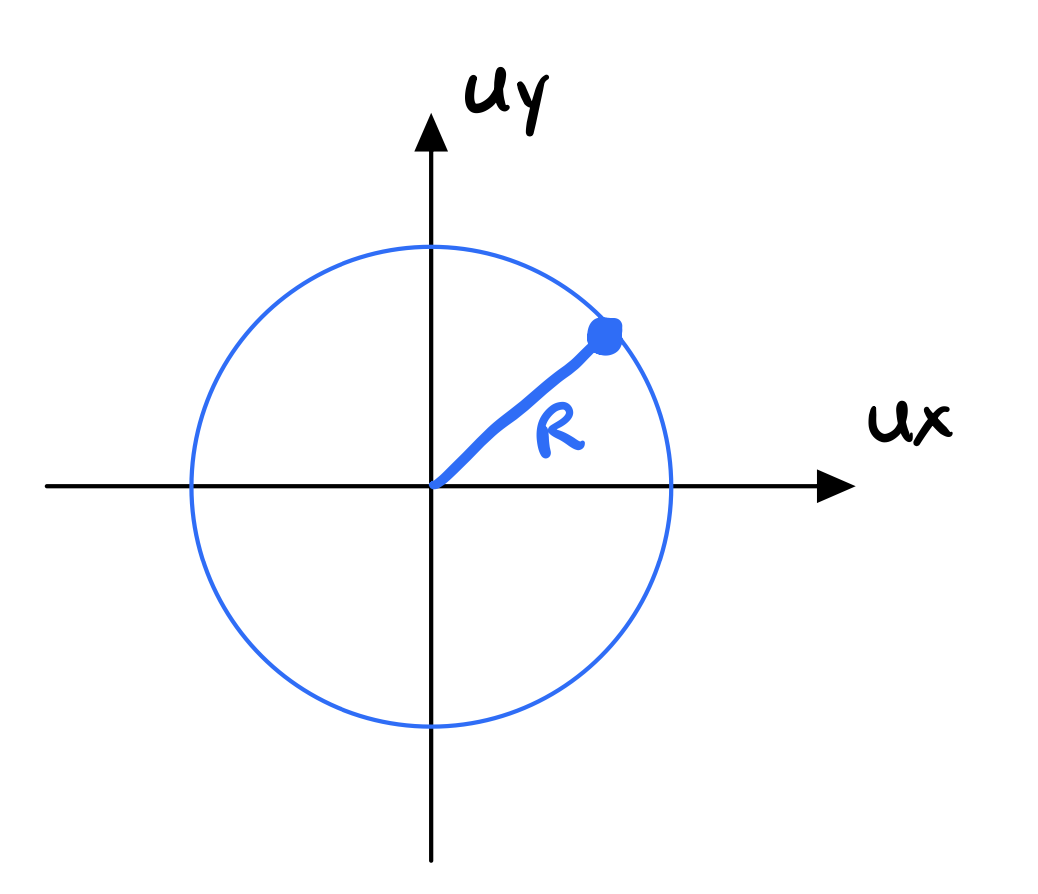
\includegraphics[scale=0.35]{Lectures/Images/lec5-uxuyspace.png}
\end{center}

Then in strain space $(S_1, S_2)$ we have a circle of radius $qR$ will be traced out over one cycle. The work done is (as we have previously calculated):
\begin{equation}
    W_{\text{odd}} = 2K^0 \cdot \text{Area} = 2K^0\pi(qR)^2
\end{equation}
Where does this energy go? We can imagine that this energy is dissipated in each cycle, so that the wave neither dies down, nor does it get amplified without bound. So, let us write down the energy being dissipated, and then balance this with the work done. The dissipated energy is:
\begin{equation}
    W_{\text{dis}} = P\Delta t = \Gamma\abs{\dot{u}}^2T = \Gamma\left(\frac{2\pi R}{T}\right)^2 T = \Gamma (2\pi R)^2 \frac{1}{T} = \Gamma R^2 2\pi \omega
\end{equation}
where $T$ is the period of the cycle. Note in the third equality that we rewrite $\dot{u}$ to be the perimeter divided by the period, and in the last equality we replace $\omega = \frac{2\pi}{T}$. Now, doing an energy balance argument, we say that the energy gained is lost by the dissipation:
\begin{equation}
    W_{\text{odd}} = W_{\text{dis}} \implies 2K^0\pi(qR)^2 = \Gamma R^2 2\pi \omega \implies \boxed{\omega = \frac{K^0}{\Gamma}q^2}
\end{equation}
Note that since the conclusion only tells us that $\omega \sim \frac{K^0}{\Gamma}q^2$ since the heuristic derivation should not necessarily give us the correct prefactor (though it does, here - a more careful derivation gives the same result). 

Note that the wave speed is given by:
\begin{equation}
    c = \frac{K^0 q}{\Gamma}
\end{equation}
so the speed of the wave scales with the wavevector/momentum $q$. Different parts of the spectrum travel at different speeds! Why no square root? We do \emph{not} have an inertial wave, where we would have two time derivatives and hence a $\omega^2$. Instead we have a dispersive wave. Note that if we take $K^0 \to 0$ (the limit of the medium becoming conservative) or take $\Gamma \to \infty$, then the wave speed goes to zero/the waves vanish.

An important note; if we have EoM $\ddot{x} = -kx$, then $k = \frac{\delta^2 U}{\delta x^2}$, we can write it as a variation of the energy. But, given that we have an odd component, $K^0_{ijmn} \neq \frac{\delta \e}{\delta u_{ij}\delta u_{mn}}$, we \emph{cannot} write it as a variation of energy. This is an example of us taking a system of solids - where traditionally everything is written as the variation of an energy - and generalizing it to a dynamical system. The dispersions we will generate as a result will have different character than what we would normally encounter in physics, either classical or quantum.

\subsection{Phonons in damped odd solids - formal argument}
Next, we want to calculate the dispersion relationship formally, and derive the phase diagram to see for what regions/phases in parameter space are phonons stable. We have equation of motion:
\begin{equation}
    \Gamma\p_t u_j = K_{ijmn}\p_i \p_m u_n
\end{equation}
we guess the ansatz:
\begin{equation}
    u_i(\v{x}) =  u_i(\v{q})e^{-i(\v{q} \cdot \v{x} + \omega t)}
\end{equation}
Leaving the algebra as an exercise, we define the parallel and transverse components:
\begin{equation}
    u_\parallel \equiv \hat{q}_i \tilde{u}_i
\end{equation}
\begin{equation}
    u_\perp \equiv \e_{ij}\hat{q}_i \tilde{u}_j
\end{equation}
then the outcome of the exercise would be:
\begin{equation}
    q_i q_m K_{ijmn}\tilde{u}_n = q^2\m{B + G & K^0 \\ -K^0 - A & G}\m{u_\parallel \\ u_\perp}
\end{equation}
If we also write the LHS in terms of $u_\parallel, u_\perp$ then:
\begin{equation}
    -i\omega \Gamma\m{u_\parallel \\ u_\perp} = -q^2\m{B + G & K^0 \\ -K^0 - A & G}\m{u_\parallel \\ u_\perp}
\end{equation}
We can then diagonalize to find the normal frequencies/modes, wherein we shall find:
\begin{equation}
    \omega = -i\left[\frac{B}{2} + G \pm \sqrt{\left(\frac{B}{2}\right)^2 - K^0A  - (K^0)^2}\right]\frac{q^2}{\Gamma}
\end{equation}
Now, the $\frac{B}{2} + G$ term corresponds to an exponential decay. It is proportional to $B, G$. There is something very subtle happening here. We perturb our solid, starting a cycle that generates energy due to $K^0, A$. The bulk and shear moduli $B, G$ do not like the cycles in strain space - from their perspective these cycles cost energy. The presence of the elastic moduli causes the damping of the waves! This is in stark contrast to oscillations that come from a potential, wherein the elastic moduli support the waves.

Going back to our expression for the frequency, the onset of active waves is whenever we have oscillatory motion of the form $e^{\pm i \text{Re}(\omega)t}$. The imaginary component can only give us decay or amplification. To get a real part, we need the square root term to be imaginary. For this, we require that the argument of the square root is negative. Thus the condition for active waves is (defining $\tilde{K}^0 = \frac{2K^0}{B}, \tilde{A} = \frac{2A}{B})$:
\begin{equation}
    \frac{B}{2}\left(1 -  \tilde{K}^0 \tilde{A} - \left(\tilde{K}^0\right)^2\right) < 0
\end{equation}
the phase transition then occurs on the hyperbola:
\begin{equation}
    \tilde{A} = \frac{1}{\tilde{K}^0} - \tilde{K}^0
\end{equation}
so we have the rough phase diagram:

\begin{center}
    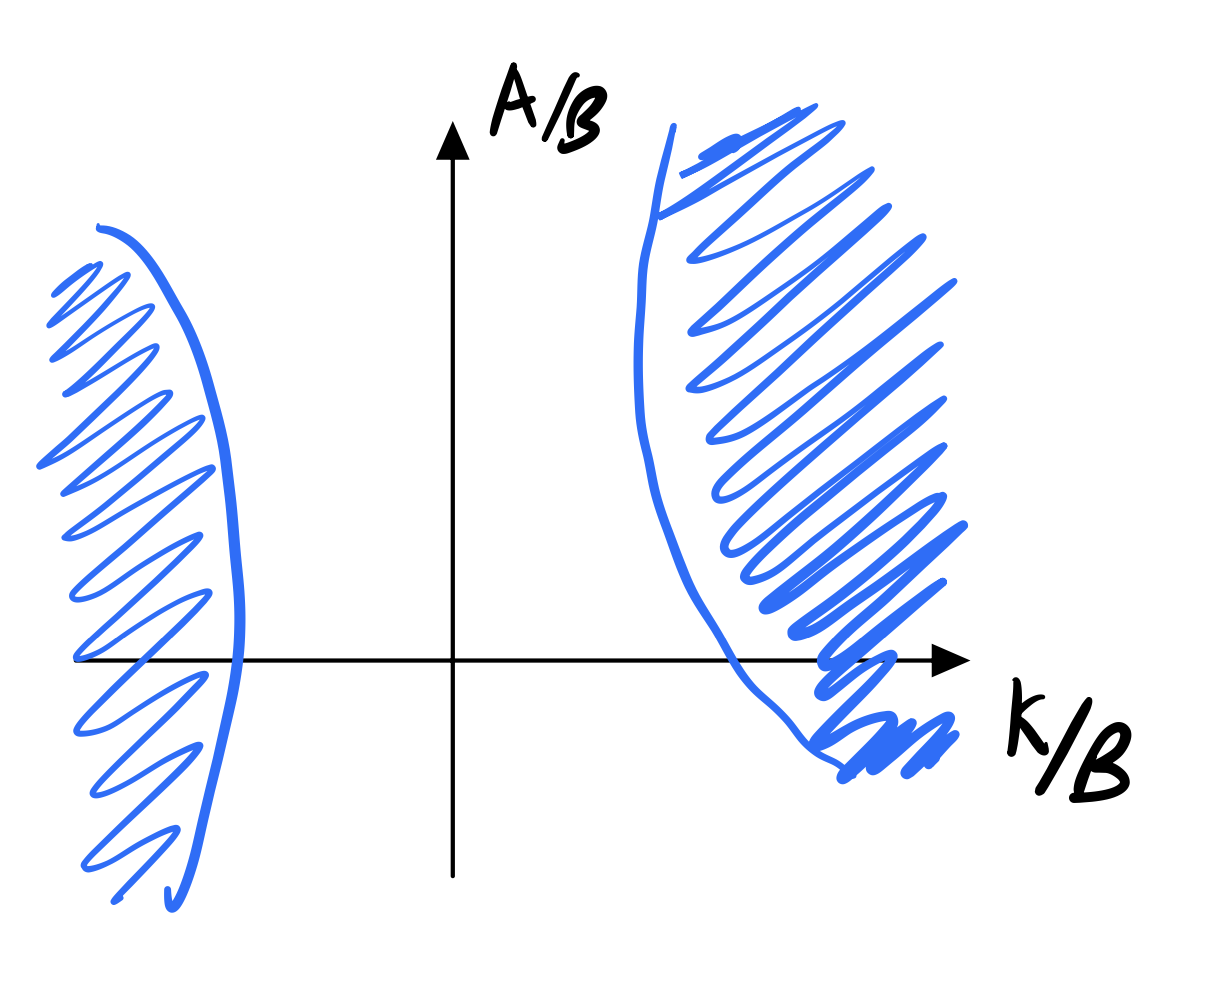
\includegraphics[scale=0.35]{Lectures/Images/lec5-phasediagram.png}
\end{center}

where in the blue regions/phases we get active waves, and in the central condition we have no propagation.

Next class we look at this phase diagram more carefully. We also look at what happens along the $ \tilde{A} = \frac{1}{\tilde{K}^0} - \tilde{K}^0$ lines and look for exceptional points. We also look at limits of large odd elastic moduli and see cases where we have amplification.
\section{Odd Elastodynamics III}

\subsection{Review}
We continue our discussion of odd elastodynamics. Last time, we considered the limit where $G, B, A \ll K^0$ and where we had overdamped dynamics. We then showed that we have oscillations with frequency:
\begin{equation}
    \omega = \frac{K^0}{\Gamma}q^2
\end{equation}
Remarkably, we get standing waves, where stress and strain are 90 degrees out of phase (Figure below taken from \url{https://www.nature.com/articles/s41567-020-0795-y}).

\begin{center}
    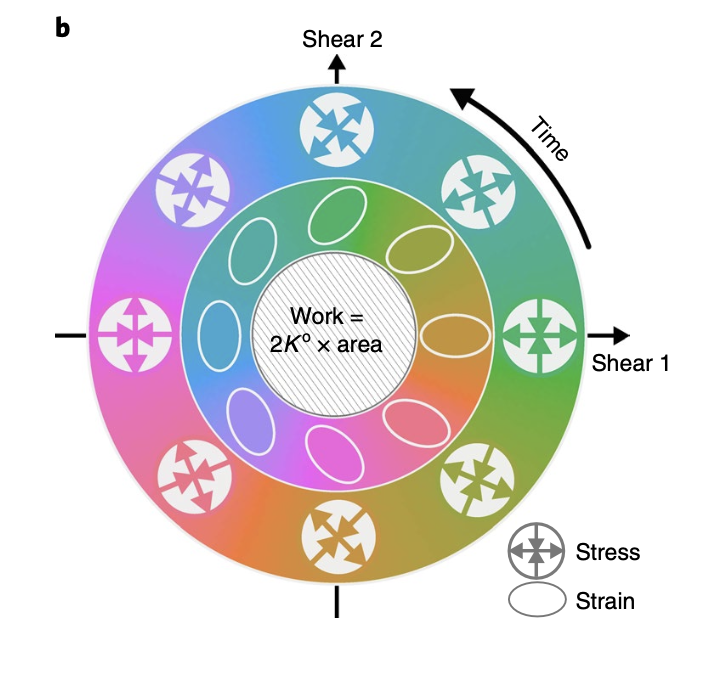
\includegraphics[scale=0.5]{Lectures/Images/lec6-oddelasticwave.png}
\end{center}

In strain space, we trace out an area, corresponding to work:
\begin{equation}
    W = 2K^0 \text{Area}
\end{equation}
with wave speed:
\begin{equation}
    c = \frac{2K^0q}{\Gamma}.
\end{equation}

Decomposing the displacements into parallel and perpendicular components:
\begin{equation}
    u_\parallel \equiv \hat{q}_i\tilde{u}_i, \quad u_\perp \equiv \e_{ij}\hat{q}_j \tilde{u}_i
\end{equation}
we obtain the relation:
\begin{equation}
    -i\omega\Gamma\m{u_\parallel \\ u_\perp} = -q^2\m{B + G & K^0 \\ -K^0 - A & G}\m{u_\parallel \\ u_\perp}
\end{equation}
which inform us about the normal modes of the elastic spectrum. We will momentarily see how the dynamical matrix for an odd solid differs from a regular one - namely the matrix is not Hermitian. We want to use the above matrix equation to solve for the eigenfrequencies and eigenvectors. Taking the determinant and setting it to zero, we find:
\begin{equation}\label{eq:oddnormalfreqs}
    \omega = -i\left[\underbrace{\frac{B}{2} + G}_{\text{decay}} \pm \sqrt{\left(\frac{B}{2}\right)^2 - K^0A - (K^0)^2}\right]\frac{q^2}{\Gamma}
\end{equation}

The decay term comes from the fact that the odd elasticity tries to deform the object, but this costs energy in terms of the bulk/shear modulus (because it strains the material). The more we pay that energy cost (i.e. larger $B, G$) the more the wave gets attenuated. Fortunately, we look at the $B, G \ll K^0$ limit; this is somewhat equivalent to studying fluid density waves in the low-viscosity limit. Microscopically this is quite odd (though there are some physical systems, e.g. Abrikosov lattices in superconductors), because this corresponds to the $\kappa \to 0$ limit of the microscopic force law $F = -(\kappa^0\hat{\gv{\phi}} + \kappa\rhat)\delta r$. 

We can study the onset of waves; this occurs when we have $e^{i\text{Re}(\omega)t}$, but this only occurs when the argument of the square root is negative. The condition we found was:
\begin{equation}
    1 - \tilde{K}^0\tilde{A} - (\tilde{K}^0)^2 < 0
\end{equation}
where $\tilde{K}^0 = \frac{2K^0}{B}, \tilde{A} = \frac{2\tilde{A}}{B}$. The locus/phase transition was given by the hyperbola:
\begin{equation}
    \tilde{A} = \frac{1}{\tilde{K}^0} - \tilde{K}^0
\end{equation}

\subsection{Instability, Phase Diagram}
Notice the heuristic argument we made based on energy balance relied on the argument that the energy produced in one cycle could overcome the dissipation lost. In particular, we set the energy gained to be equal to that lost. If the energy gained was less, then the wave would die out. If the energy gained was more, then instead we would have an instability/the wave amplitude would continue to grow.

Let's look at the region of this instability more carefully. This occurs when the spectrum acquires a positive imaginary branch. In particular, we look for a situation where $e^{\Im(\omega)t}$ with $\Im(\omega) > 0$, then we have exponential amplification in time. We require:
\begin{equation}
    \frac{B}{2} + G - \sqrt{\left(\frac{B}{T}\right)^2 - K^0A - (K^0)^2} < 0
\end{equation}
then the crossover happens when:
\begin{equation}
    \left(1 + \tilde{G}\right)^2 = 1 - \tilde{K}^0\tilde{A} - (\tilde{K}^0)^2
\end{equation}
i.e.:
\begin{equation}
    \tilde{A} = -\frac{2\tilde{G} +\tilde{G}^2 + (\tilde{K}^0)^2}{\tilde{K}^0}
\end{equation}
Note that we know that we have instability after this point - we don't know what happens after this (whether we get nonlinear excitations, or whether the lattice begins to melt/crumble etc...)

With this region discussed, we can now understand the entire phase diagram (figure taken from \url{https://www.nature.com/articles/s41567-020-0795-y})

\begin{center}
    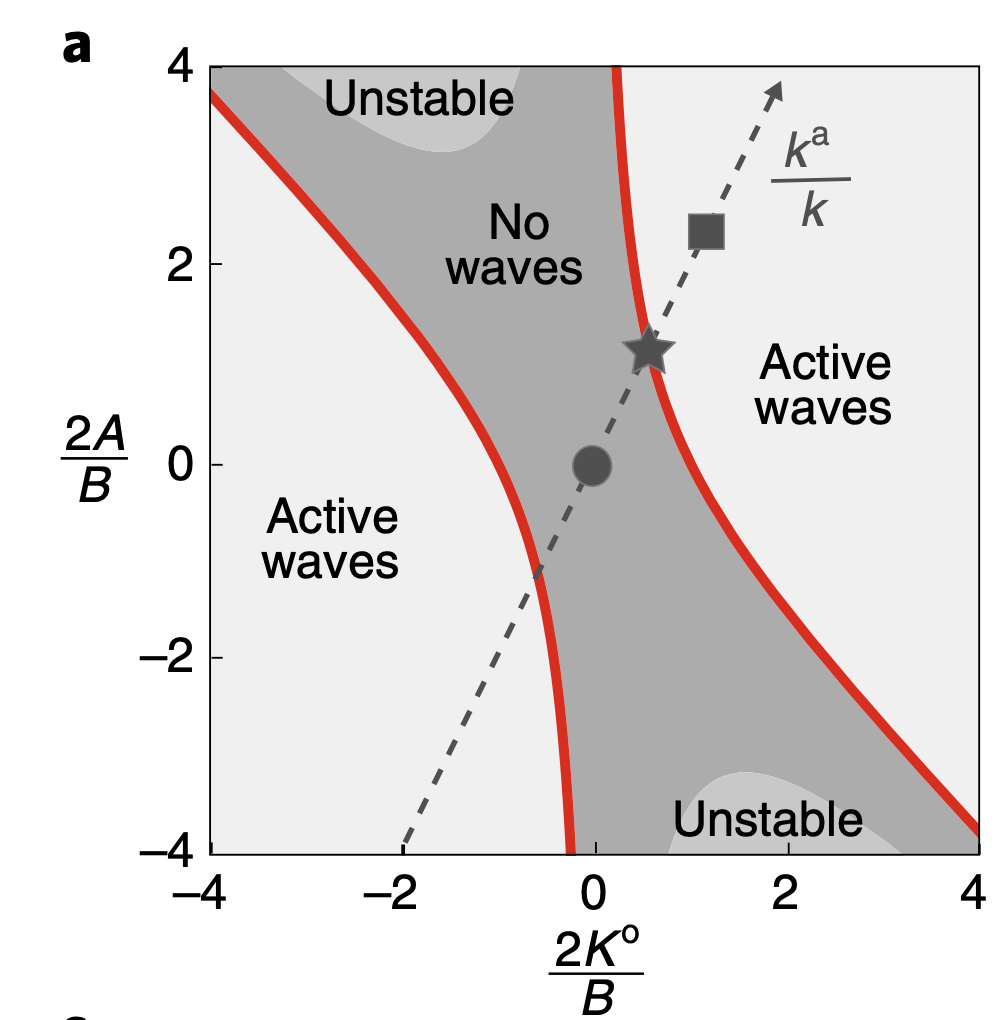
\includegraphics[scale=0.5]{Lectures/Images/lec6-oddelasticphasediagram.png}
\end{center}

A comment; if we had assumed a microscopic force model of $F = -(\kappa^0\hat{\gv{\phi}} + \kappa \rhat)\delta r$, we could course grain to find the dependencies of $A, K^0, B$ on the microscopic parameters, and then the knowledge of the microscopic parameter ratio $\frac{\kappa^0}{\kappa}$ would be able to tell us about where in the phase diagram we were located.

Another comment about instability: even if we have a linear microscopic constitutive equation, we could potentially get macroscopic non-linearities coming out of rotations (only 2-d and up - coming from the last term):
\begin{equation}
    u_{ij} = \p_i u_j + \p_j u_i + \p_k u_i \p_k u_j.
\end{equation}



\subsection{Exceptional Points}
Now, let's talk about what happens on the dashed line of the phase diagram when we cross from the active to the no wave region (star point). We have the $\omega$ from Eq. \eqref{eq:oddnormalfreqs}, and can also compute the eigenvectors. Before, this, a comment about the dynamical matrix - It is not Hermitian if $A, K^0 \neq 0$. This means that the convenient properties - real eigenvalues, orthogonal eigenvectors - are lost. In QM this is necessary for real measurement outcomes and conservation of probability. But for open quantum systems, we require non-Hermitian matrices. 

Let's compute the eigenvectors and see that they are non-orthogonal:
\begin{equation}
    u_i = \frac{(1 \pm \sqrt{1 - \tilde{K}^0\tilde{A} - (\tilde{K}^0)^2})\hat{q}_i - (\tilde{A} + \tilde{K}^0)\e_{ij}\hat{q}_j}{\sqrt{2(1\pm\sqrt{1 - \tilde{K}^0\tilde{A} - (\tilde{K}^0)^2}) + \tilde{K}^0\tilde{A} + (\tilde{K}^0)^2}}
\end{equation}
Unwieldy, but you might be able to convince yourself that we only get orthogonality if $\tilde{K}^0 = A = 0$.

With this obtained we can discuss what happens at the onset of odd waves. There is a point called the \emph{exceptional point}\footnote{In this age of exceptionalism, Vincenzo must apologize and say that this is not that exceptional.}. It is a statement about the fact that a singularity occurs.

\begin{enumerate}[(a)]
    \item We can see from Eq. \eqref{eq:oddnormalfreqs} that at the exceptional point when $\tilde{A} = \frac{1}{\tilde{K}^0} - \tilde{K}^0$ that the square root term is zero and that the spectrum acquires a degeneracy, where the eigenvalues become the same:
    \begin{equation}
        \omega = -i\left[\frac{B}{2} + G \pm 0\right]
    \end{equation}
    \item What happens to the $u_+, u_-$ eigenvectors at this point? They become collinear!
\end{enumerate}

We will encounter these exceptional points again when we study non-reciprocal phase transitions.

\subsection{Poisson Ratio and Odd Ratio}
Imagine we could measure the spectrum of the odd waves; we would be able to measure $\tilde{K}^0, A, \frac{B}{2}, G$ etc. This would be a dynamical measurement. You might also ask - why could we not do a static measurement? Indeed we could just compress/apply forces to the solid in different ways, and just see how it deforms.

We can consider the Poisson ratio:
\begin{equation}
    \nu = -\frac{u_{xx}}{u_{yy}}
\end{equation}
in normal materials, $\nu > 0$ and so if we compress one way, it expands in the other direction. In auxetic materials (e.g. metamaterials like rotating triangular auxetic perforated plates), we have $\nu < 0$ so if we compress it compresses in the other direction too! There is also the case of $\nu \approx 0$, e.g. cork where we compress in one direction and the other direction basically does not change. 

What about odd materials? we compress in one direction and then there is a response to an angle. This violates parity - and hence requires parity violating moduli. Note that in this case it is useful to define the odd ratio:
\begin{equation}
    \nu^0 = \frac{K^0B}{(K^0)^2 + G^2 + BG}
\end{equation}
which characterizes the angle at which the material deforms when compressed.

Next time, we look at the case where linear momentum conservation is violated. Then we turn to fluids without viscosity, in particular turbulence in non-viscous fluids.
\section{Odd Elastodynamics IV}

We study the overdamped limit:
\begin{equation}
    \Gamma \p_t u_i = F_i = \p_j \sigma_{ij} = \p_j (K_{ijkl}u_{kl}) = K_{ijkl}\p_j\p_l u_k
\end{equation}
In the space of shears:
\begin{equation}
    \Gamma \p_i \m{u_x \\ u_y} = \m{G & -K^0 \\ K^0 & G}\m{\nabla^2 u_x \\ \nabla^2 u_y}
\end{equation}
or in more full generality, after Fourier transforming and looking at the parallel/perpendicular (to the wavevector) components:
\begin{equation}\label{eq:dynamical}
    -i\Gamma \omega\m{u_\parallel \\ u_\perp}  = q^2\m{B + G & K^0 \\ -K^0 - A & G}\m{u_\parallel \\ u_\perp}
\end{equation}
By studying this eigenvalue problem, we get the plot:
\begin{center}
    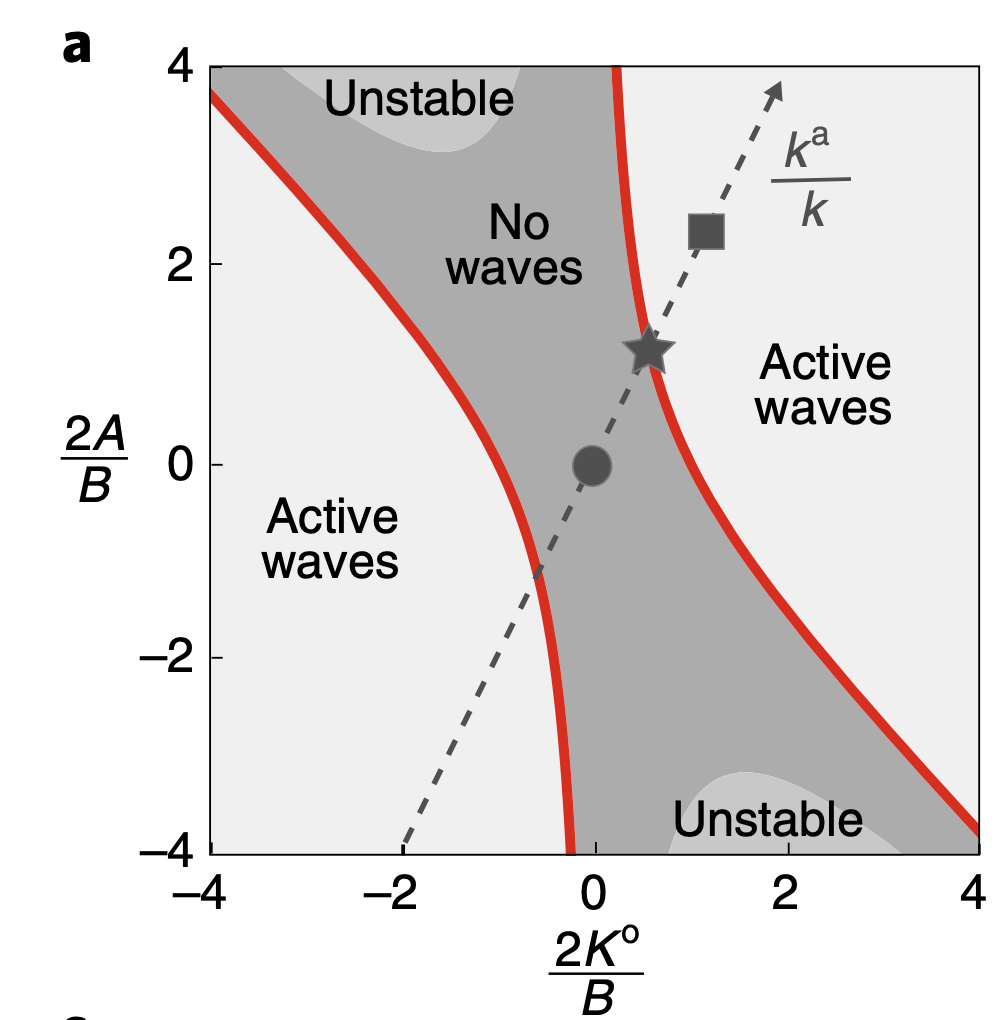
\includegraphics[scale=0.5]{Lectures/Images/lec6-oddelasticphasediagram.png}
\end{center}
We call the propagating waves ``active waves'' as they are propagated by the cycles arising from the odd elastic moduli.

The red lines that separate the regions where the waves do not propagate are called ``exceptional lines'', meaning they consist of exceptional points - the two eigenvalues of the dynamical matrix become degenerate, and the two corresponding eigenvectors become collinear. It is worth noting that the dynamical matrix we have written down in Eq. \eqref{eq:dynamical} is Non-Hermitian (as you may have seen in open quantum systems), and thus the eigenvectors are not orthogonal (and in particular the angle between them goes to zero at the exceptional points).

\subsection{Topological Defects/Dislocations}
We saw some examples last class of auxetic and odd materials. Another system of interest are crystals with topological defects, which exhibit novel behaviour in the presence of stresses. In your homework you do this for the case without odd elastic moduli, but the calculation can also be done in the $K^0 \neq 0$ case, and such behaviour has also been observed by a group at MIT.

In lecture, we watched a video first of rays propagating through a compressed triangular crystal. We then zoomed into it, and saw that it was perfect save for a dislocation where we have made the coordination number 7/5 as opposed to 6. This defect gives rise to an extra row of atoms; for any loop surrounding the defect we are able to detect this extra step. The rays we saw moving through the crystal arose from the ray-like motion of the defects arising from applying a (shear) stress/perturbation to the lattice. 

\begin{center}
    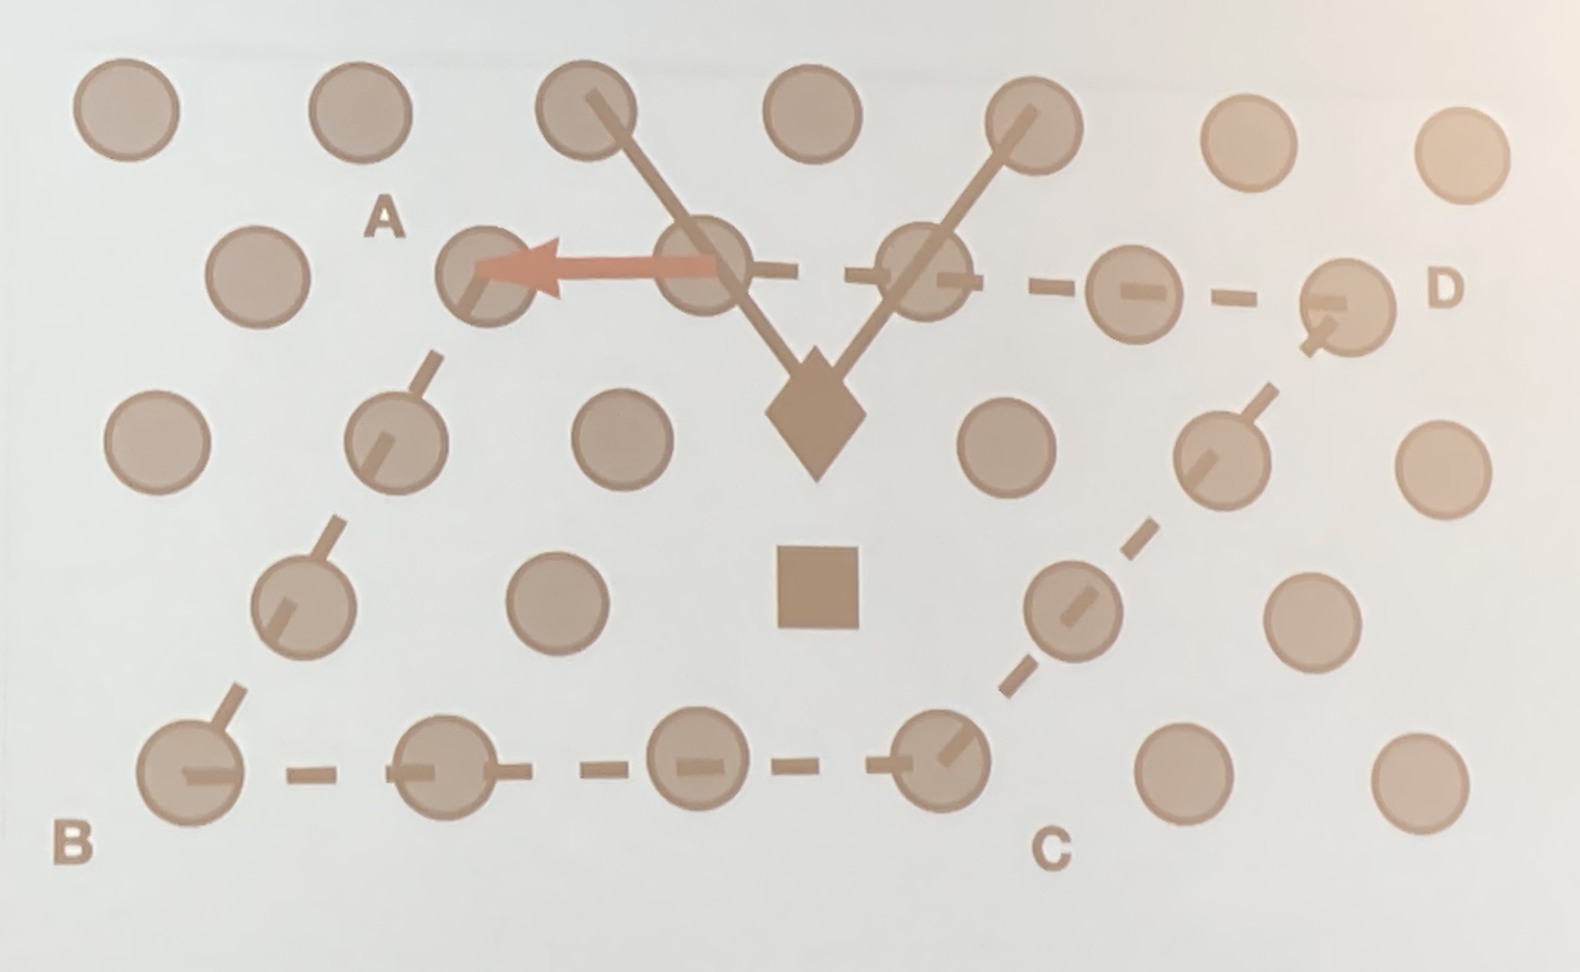
\includegraphics[scale=0.3]{Lectures/Images/lec7-dislocationatoms.png}
\end{center}
Mathematically, the dislocation (which are analogous to magnetic monopoles) is characterized by the Burges vector, where we do a loop integral around the dislocation:
\begin{equation}
    \v{b} = \oint_{\gamma}d\v{r} \cdot \nabla \v{u}
\end{equation}
Then using the force balance condition:
\begin{equation}
    0 = \v{f} = \nabla \cdot \gv{\sigma}
\end{equation}
We have the displacement field:
\begin{equation}
    \v{u}(\v{r}) = \frac{1}{2\pi}\left[\phi \v{b} + \frac{1-\nu}{2}\log(r)\gv{\e} \cdot \v{b} - \frac{1+\nu}{2}\rhat \cdot \v{b}\hat{\gv{\phi}} - \nu^0\left[\log(r)\v{b} + \hat{\gv{\phi}}\cdot \v{b}\hat{\gv{\phi}}\right]\right]
\end{equation}
where the last term is the odd term, with odd ratio:
\begin{equation}
    \nu^0 = \frac{BK^0 - AG}{G(B + G) + K^0(A+K^0)}
\end{equation}
this is zero for a regular crystal (the case you study in your homework), but the odd case was studied theoretically by Lara Braverman and Colin Scheibner, as you can read about in \url{https://journals.aps.org/prl/abstract/10.1103/PhysRevLett.127.268001}. A couple of years later, a team at MIT used the proposal in this Letter to do an experiment with spinning colloids \url{https://www.nature.com/articles/s41586-022-04889-6}, where they tried to extract the odd elastic parameters from the shear angle (though the experimental data is very noisy...).

An equation that we will not derive, but use, is that of the Peach-Koehler (PK) force. It is the analog of the Lorentz force in EM theory:
\begin{equation}
    F_i = q\e_{ijk}v_jB_k
\end{equation}
this is an example of manifest parity violation that you are very familiar with - cyclotron orbits are in a particular direction. There is a mathematically analogous force for dislocations:
\begin{equation}
    F_i^{PK} = -\e_{ij}b_k\sigma_{jk}
\end{equation}
which tells you about the force on the dislocation (characterized by the Burges vector $\v{b}$) as a result of an applied stress. This force is highly orientation dependent.

The crucial feature of the experimental results using spinning colloids is that there are pre-torques/stresses (which violate angular/linear momentum conservation) in $\sigma_{ij}$:
\begin{equation}
    \sigma_{ij} = \underbrace{\tau_0 \e_{ij}}_{\text{pre-torque}} + \underbrace{p\delta_{ij}}_{\text{pre-stress}} + K_{ijkl}\p_k u_l
\end{equation}
If we put the pre-torque into the PK force equation:
\begin{equation}
    F_i^{PK} = -\e_{ij}b_k\tau^0\e_{jk} = \delta_{ik}b_k\tau^0
\end{equation}
where we have used $-\e_{ij}\e_{jk} = \delta_{ik}$. So, we have a force along the direction of the Burges vector, proportional to the pre-torque density $\tau^0$.

One last comment that we won't have time for - in the Braverman/Scheibner PRL, we have formulas are derived from continuum mechanics - but the Burges vector is a dislocation arising from meso/microscopic phenomena. These details can actually lead to the breakdown of the field-theoretic description, and lead to a reversal in the direction of the force as predicted by the field theory formula. Sometimes we can learn as much from the cases where field theory holds, as well as where it breaks down! In particular, here the field theoretic description holds if defects interact at far field, but breaks down if defects become close.

\subsection{Relaxing linear momentum conservation}
All of our discussion thus far has arose because we relaxed the assumption of energy conservation. However, throughout we have been assuming:
\begin{equation}
    F_i = \p_j \sigma_{ij}
\end{equation}
which assumes that the medium conserved linear momentum (the above is the divergence of a flux of linear momentum). This is what gave rise to the force being the second spatial derivative of the displacement/strain.

However, it is possible to write a more general force law, if we relax the conservation law. Let us expand $F_i$ in a general way, expanding in gradients of the deformation:
\begin{equation}
    F_i = \alpha u_i + \beta_{ijk}\p_j u_k + K_{ijkl}\p_j \p_l u_k
\end{equation}
Let's consider a simple solid that violates Newton's third law\footnote{There is a 2025 PNAS paper by Bartolo, Vitelli, Irvine and others that discusses this - and the classification of $\beta_{ijk}$, if you wanted to read more about it.}. We want no adhesion forces, so we drop the first term:
\begin{equation}
    F_i = \beta_{ijk}\p_j u_k + K_{ijkl}\p_j \p_l u_k
\end{equation}
This could be, for example, a fluid that moves through a collection of colloids/droplets. This clearly violates Newton's third law because there is a preferred direction/the colloids feel different forces against/along the fluid flow. A toy model that can describe this would be a chain of 1D masses connected by non-reciprocal (asymmetric) springs:

\begin{center}
    
\includegraphics[scale=0.4]{Lectures/Images/lec7-NRspringchain.png}
\end{center}

In this 1-D case, the equation of motion reduces to (still working in the overdamped limit):
\begin{equation}\label{eq:neweom}
    \gamma \p_t u = \beta \p_x u + \kappa \p_x^2 u
\end{equation}
simple as this looks, this is still quite different from the standard wave equation that is studied in the context of solids:
\begin{equation}
    \rho \p_t^2 u = \kappa \p_x^2 u
\end{equation}
wherein the speed of sound is $c = \sqrt{\frac{\kappa}{\rho}}$. The fourier transform of this yields the dispersion relation:
\begin{equation}
    \omega^2 = c^2q^2 = \kappa q^2
\end{equation}
(Where we work in units where $\rho = 1$), or:
\begin{equation}
    \omega(q) = \sqrt{\kappa}\abs{q}
\end{equation}
Note then that:
\begin{equation}
    \omega(q) = \omega(-q)
\end{equation}

Let's also try studying the spectrum for Eq. \eqref{eq:neweom}; fourier transforming (equivalently, using the wave ansatz $u(x, t) = Ae^{i(qx + \omega t)}$). We find:
\begin{equation}
    \gamma i \omega = i q \beta - \kappa q^2
\end{equation}
Or multiplying by $-\frac{i}{\gamma}$:
\begin{equation}
    \omega = \frac{\beta}{\gamma}q + i\frac{\kappa}{\gamma}q^2
\end{equation}

There is a propagating wave term coming from $\frac{\beta}{\gamma}q$, and there is a piece that is attenuating $i\frac{\kappa}{\gamma}q^2$. The part that should draw your attention is that $\omega(q)$ - is \emph{not} invariant under $q \leftrightarrow -q$. Indeed in the $\kappa \to 0$ limit $\omega(q)$ is actually odd under this transformation:
\begin{equation}
    \omega(q) = -\omega(-q)
\end{equation}
The non-reciprocity/breaking of mirror symmetry is what enables this strange feature of the spectrum.
\section{Self-Propelled Particles/Polar Active Fluids}

\subsection{Overview of Self-propelled particles}
Today we discuss self-propelled particles, also known as polar active fluids. Your next homework will be almost entirely devoted to this topic. This is a new type of active matter, compared to what you have seen thus far in the course. The first experiments on this topic can be found in \texttt{Pallaci et al.\ Science (2014)}, \texttt{Bricard et al.\ Nature (2013)}.

Those in the soft matter class will know that there is one equation that governs the dynamics of simple fluids, namely the Navier-Stokes equation. Those not in the course will learn a bit of simple and complex fluids on the fly.

To give a bit of a physical picture, we are imagining that we have a fluid channel, containing many colloids. In the absence of pressure gradient, we see Brownian motion, and in the presence of a pressure gradient, we will see colloid flow. Here we consider the possibility of ``active colloids''. One example - colloids can have assymmetry (``Janus Particles''), e.g. the two sides can be made up of different material. If we shine light on the particles, the different sides will heat up in different amounts, creating a gradient within the particle itself. It then acts like a rocket that launches fuel more in one direction than the other, triggering the motion.

Another example (which you will become intimately familiar with on the homework) - we can have colloidal rollers that can be polarized via an electric field. Then, by rotating the colloids, we can have the colloids individually flow. If we have a fluid of such colloids, they will want to roll and align with each other - thus without applying any pressure gradient (they are self-driven!), the colloids will spontaneously pick a direction and flow. We will want to derive and analyze the Navier-Stokes equations to describe such self-propelled fluids. On your homework, you will first see how you can get a single particle to self-propel. Then, you will study the linear spectrum/excitations of such a medium. Finally, you will look at non-linear excitations, wherein the colloidal rollers move with a band structure.

You might imagine that there are interesting microfluid experiments that could be done with such exotic fluids. You can engineer lattices to contain such active fluids, and study what the properties of such a lattice are. In a Lieb lattice, such rollers rotate with alternating directions (chirality)! 

\begin{center}
    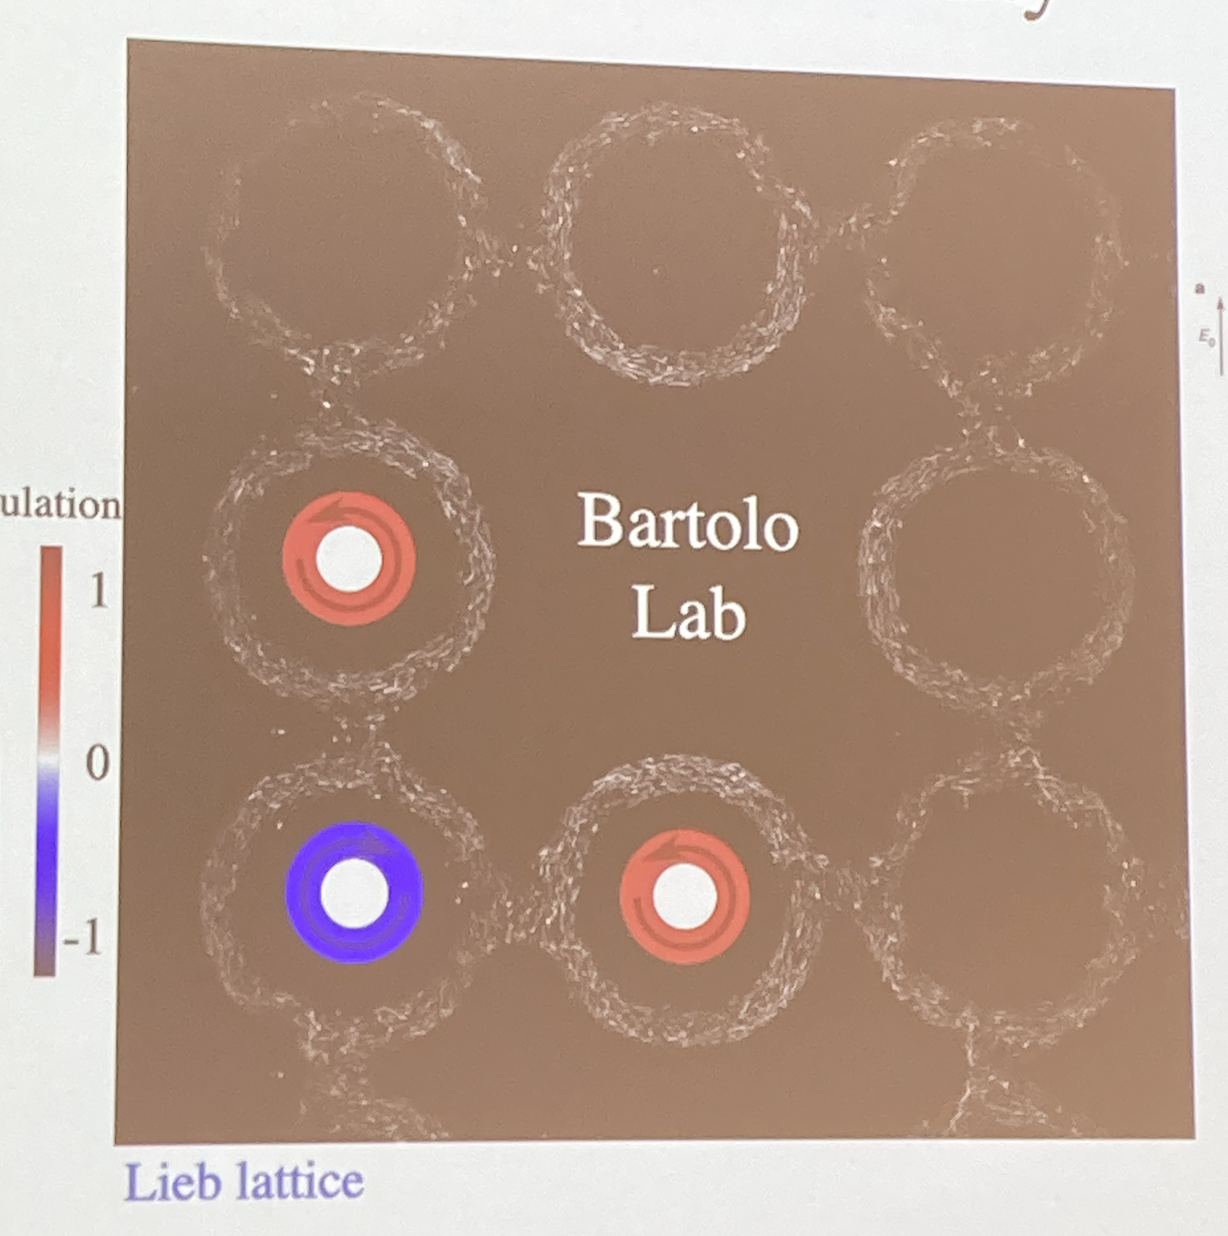
\includegraphics[scale=0.35]{Lectures/Images/lec8-circulation.png}
\end{center}

You can then also study what the sound modes of a channel made of such a fluid would look like - this your task in the homework, to look at density modulations on top of a nonzero velocity field. The sound waves will have a strange structure - density waves that go along with the flow and against the flow will have very different behaviours. You can even put this problem on steroids (\texttt{Souslov, van Zuiden, Bartolo, Vitelli.\ Nature (2017)}), and study such waves in not just one channel but in a 2D lattice - it turns out you can make a topological insulator out of such a lattice! Looking at the band structure, the bulk is gapped. But at the edge, you can have a density wave/excitations, and it is a directed excitation; it travels in a specific direction. In fact such excitations are topologically robust, in that they can flow around obstructions.

\begin{center}
    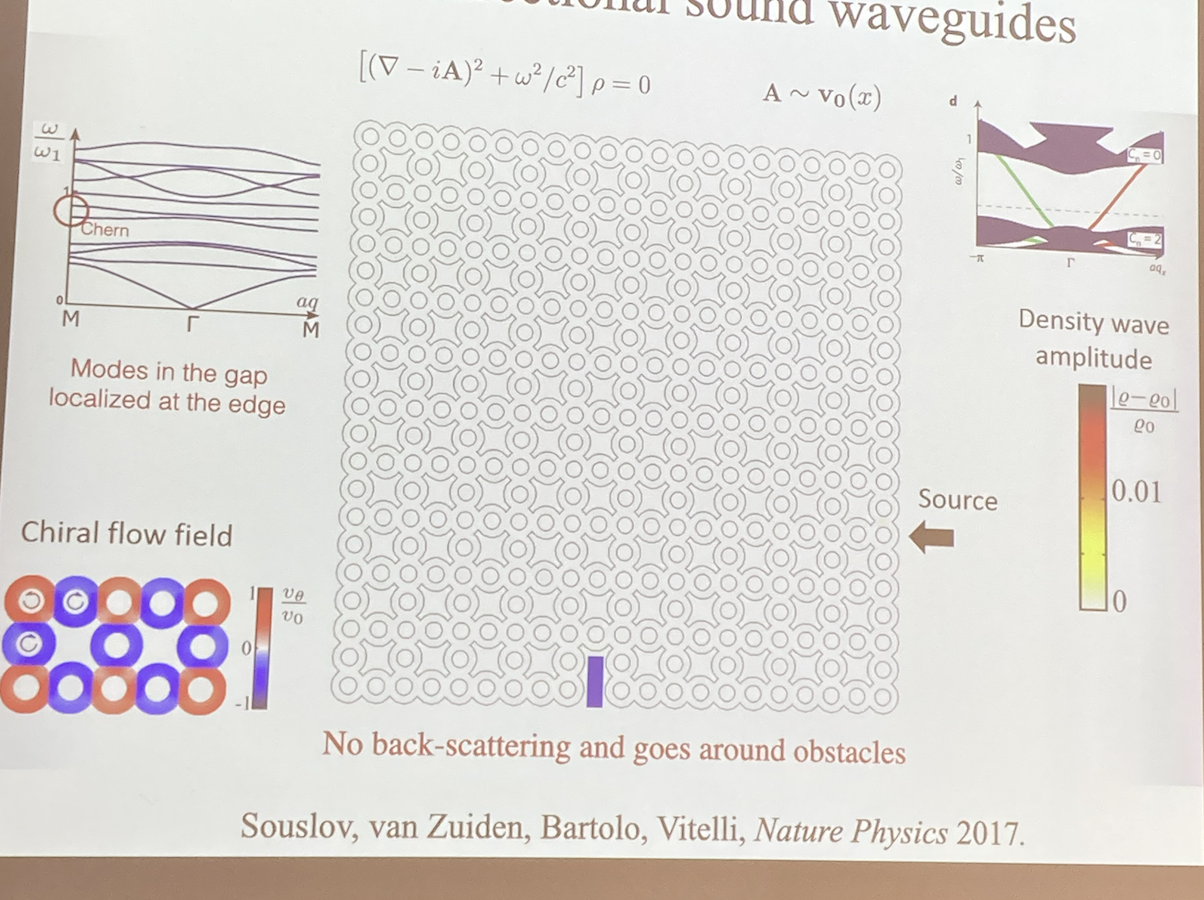
\includegraphics[scale=0.35]{Lectures/Images/lec8-lattice.png}
\end{center}

\subsection{Vicsek Model}
We will study the microscopic model that started this field - the Vicsek model of flying spins. The hydrodynamics of this model shows flocking\footnote{Everyone calls this flocking, but no one asked how the birds feel about it...} behaviour and phase transitions, and will be a useful model for understanding the more contemporary models of active matter that have come after it.

We consider a collection interacting bodies, and consider a mechanism in which the bodies move and align align. Consider the picture below:

\begin{center}
    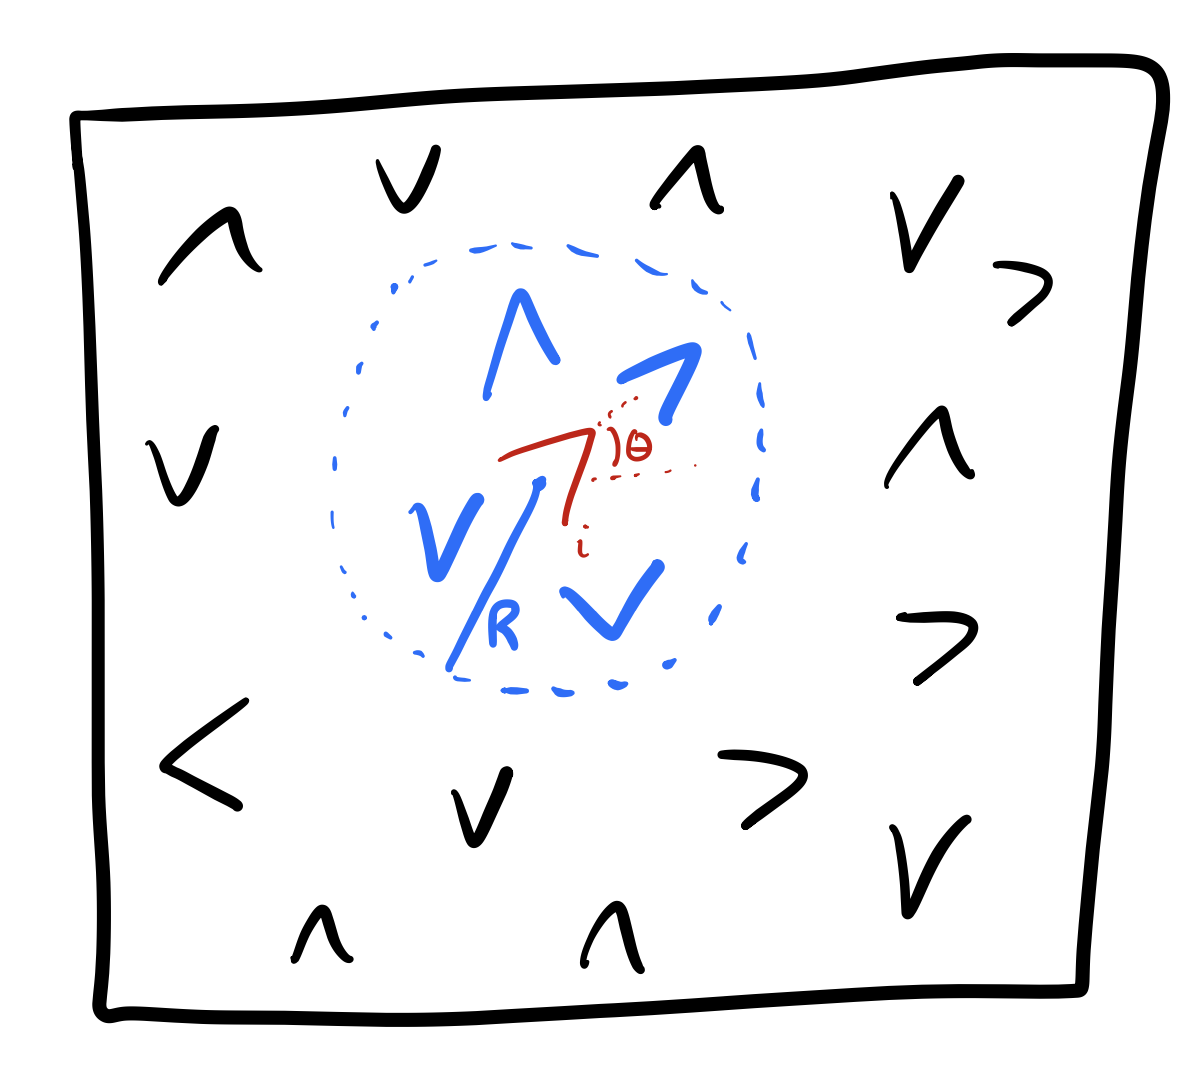
\includegraphics[scale=0.35]{Lectures/Images/lec8-Vicsek.png}
\end{center}

The update rule for the position of the $i$th body is:
\begin{equation}
    \v{r}_i(t + \Delta t) = \v{r}_i(t) + v_0\Delta t\m{\cos(\theta_i(t)) \\ \sin(\theta_i(t))}
\end{equation}
i.e. it takes one step in the direction it is facing. The update rule for the angle/direction of the $i$th body is:
\begin{equation}
    \theta_i(t + \Delta t) = \avg{\theta(t)}_{R, i} + \eta_i(t)
\end{equation}
where the first term corresponds to taking the average over the interaction range $R$ of other bodies. $\eta_i(t)$ is a noise term. In the Vicsek model, we can assume that the noise has zero mean:
\begin{equation}
    \avg{\eta_i(t)} = 0
\end{equation}
and has correlation (time average):
\begin{equation}
    \overline{\eta_i(t)\eta_j(t')} = 2\gamma\delta_{ij}\delta_{tt'}
\end{equation}
i.e. the noise is uncorrelated across space and time. The noise is local and Markovian (no memory), sometimes this is also called white noise.

Why is it called flying spins? The alignment of the direction of the bodies is like magnetic/spins which want to align with their neighbours, plus thermal fluctuations. The non-equilibrium dynamics comes from the fact that the spins can move! If the spins were fixed, you can just take the second equation and write down an equlibrium field theory (namely the XY model). But by coupling it into a self-propulsion rule, the model is non-equilibrium! 2D is interesting because the Mermin-Wagner theorem prevents the long-range ordering of the entire system in equilibrium settings.

Vicsek then studied this model just by numerically simulating it (this would be a good thing for you to also simulate as an exercise!) - see \texttt{Vicsek et al.\ PRL (1995)}

For high noise, we are in the disordered phase where the various spins fly in seemingly random directions. In the low noise, we are in the ordered/flocking phase where all spins move in the same direction. In this phase, we have a nonzero net velocity vector.

\begin{center}
    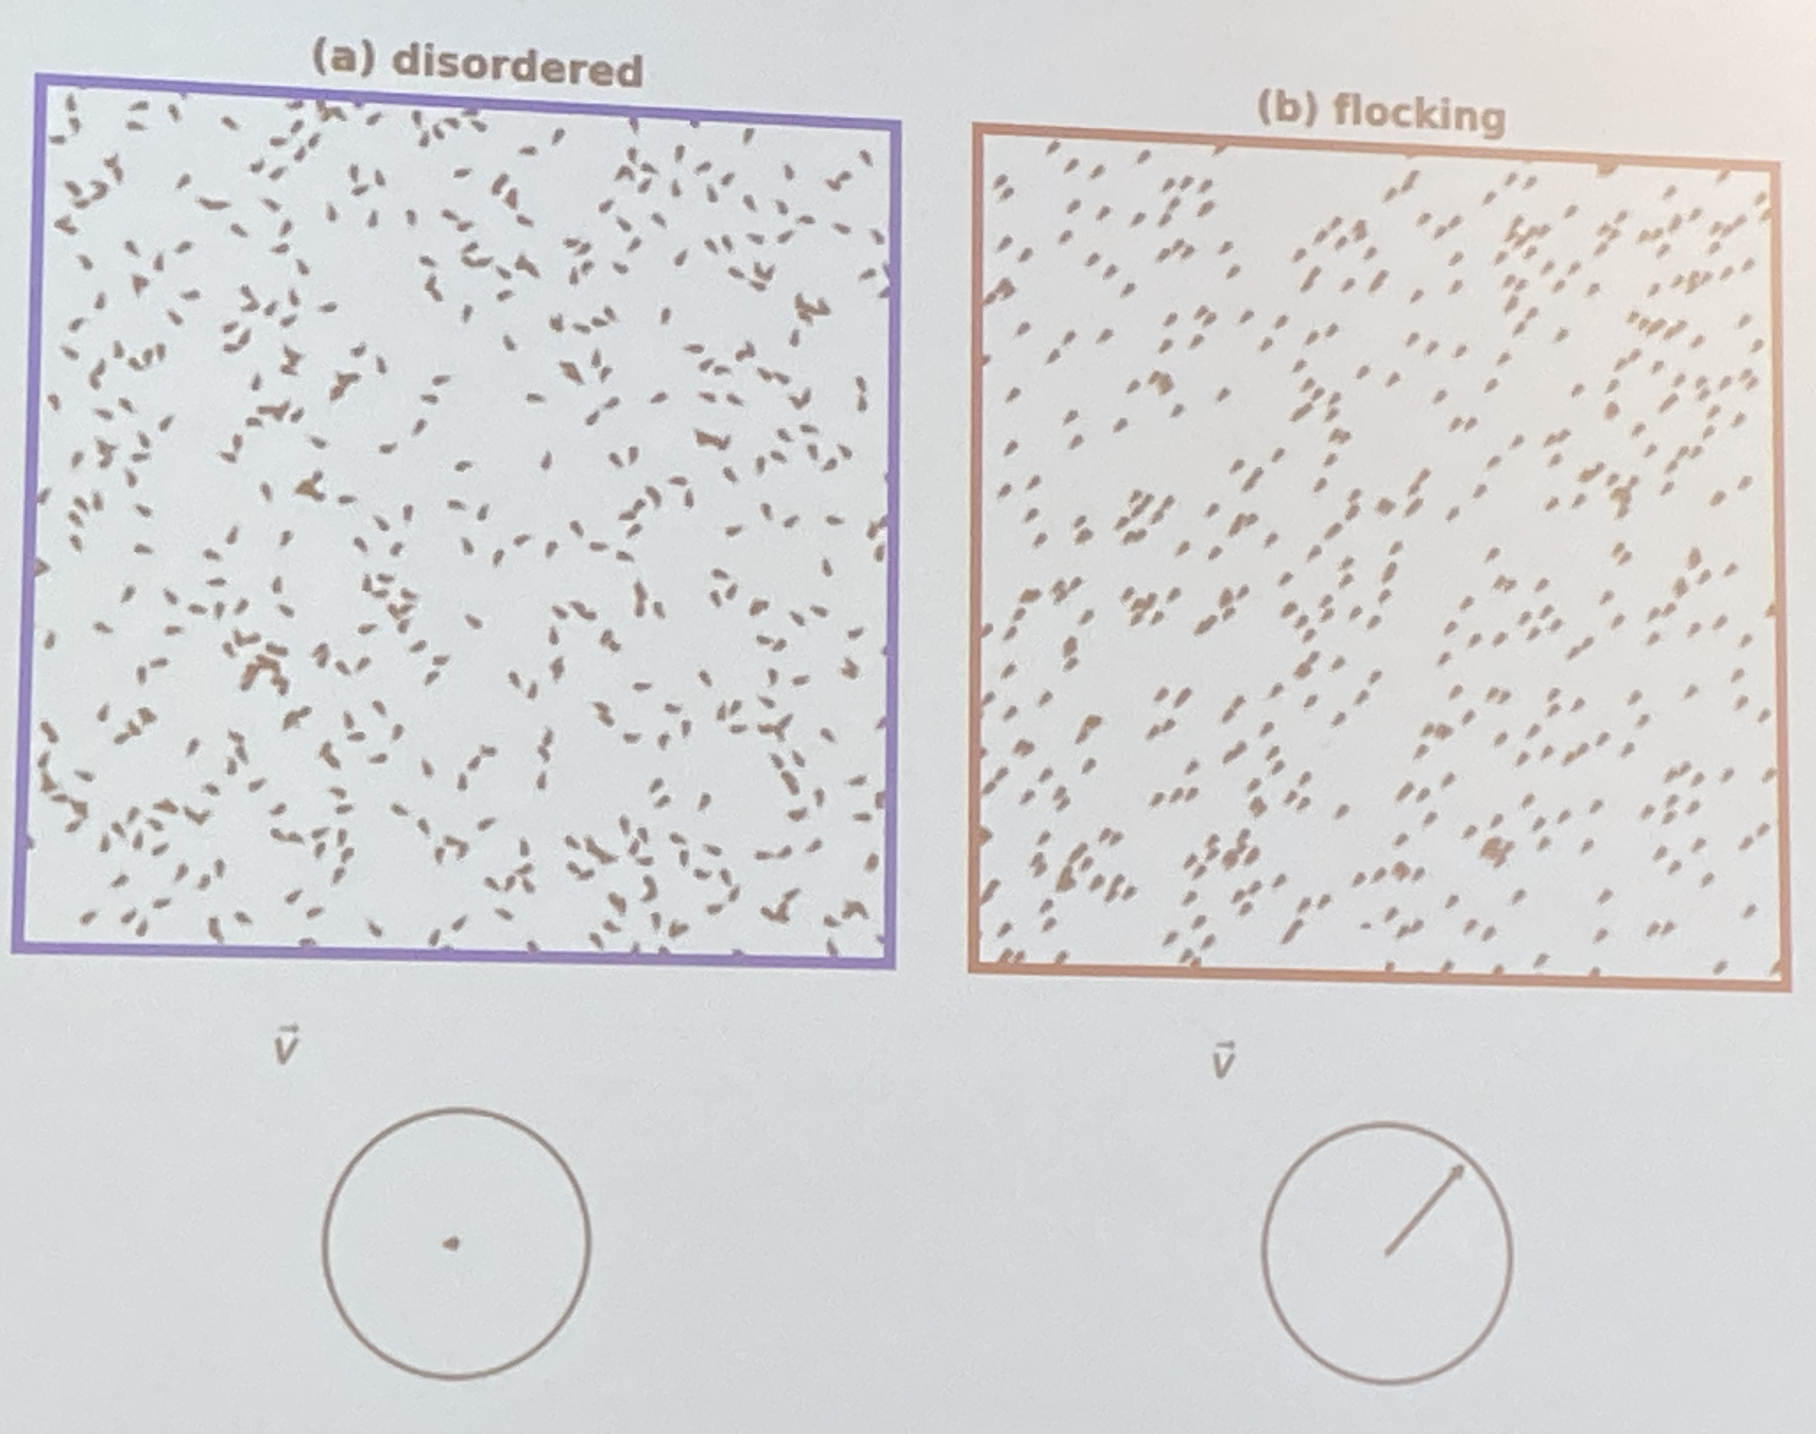
\includegraphics[scale=0.35]{Lectures/Images/lec8-flocking.png}
\end{center}

If we wanted to promote this to a continuum description, we could write down the energy:
\begin{equation}
    E = J\int d^2\v{x}(\nabla \theta)^2
\end{equation}
If $\frac{J}{k_B T} \ll 1$, thermal fluctuations are strong and we have disorder. For $\frac{J}{k_B T} \gg 1$, it is less clear. In equilibrium settings, in 2D Mermin-Wagner forbids long-range order. But here we have the coupling of the XY spin model to the self-propulsion model, which allows for the restoration of long-range order!

\subsection{Toner-Tu Model}
See \texttt{Toner, Tu.\ PRL (1995)} for the original paper.

Now, we will do some phenomenology; we will use the known symmetries of the theory and write down a macroscopic theory. As long as we are smart about it, we will get sensible results. However, we will not get the correct parameter dependencies of the macroscopic model on the microscopic parameters. Let us proceed. What we notice is that depending on the ratio $\frac{J}{\eta}$, we have either disordered or ordered behaviour. If you have taken a course on statistical field theory, you would have seen Landau theories of phase transitions, where we can write down an energy landscale that depends on a continuum spin parameter:
\begin{equation}
    E = J\int d^2\v{x}\left[(\nabla S)^2 + \alpha S^2 + \beta S^4\right]
\end{equation}
In the limit where $S$ is uniform, the gradient drops out. Then, depending on the $\alpha$ we either have a single minimum at $S = 0$ or degenerate minima at $S = \pm S_0$ (in 2D, we promote the two degenerate minima to a ring of minima, imagine a Sombrero). We can write $\alpha = c(T - T_c) = -c\e$, wherein for $T > T_c$ we have a single mimima and $T < T_c$ we have the degenerate minima. Usually in Landau theory we think about the system being in the energy minimizing configuration. We can also think about the dynamics at which the system comes to an energy minimizing configuration:
\begin{equation}
    \p_t S = -\frac{\delta V(S)}{\delta S}
\end{equation}

In our case, instead of a continuum spin/magnetization we instead have a velocity field. We have the potential:
\begin{equation}
    V(\v{v}) = -\alpha \v{v}^2 + \beta \v{v}^4
\end{equation}
Which taking the variation we get:
\begin{equation}\label{eq:TTbifurcationterms}
    \rho \p_t \v{v} = \alpha \v{v} - \beta \abs{\v{v}}^2 \v{v}
\end{equation}
This describes the bifurcation, but not the fluid aspects of the system. The pictures look like:

\begin{center}
    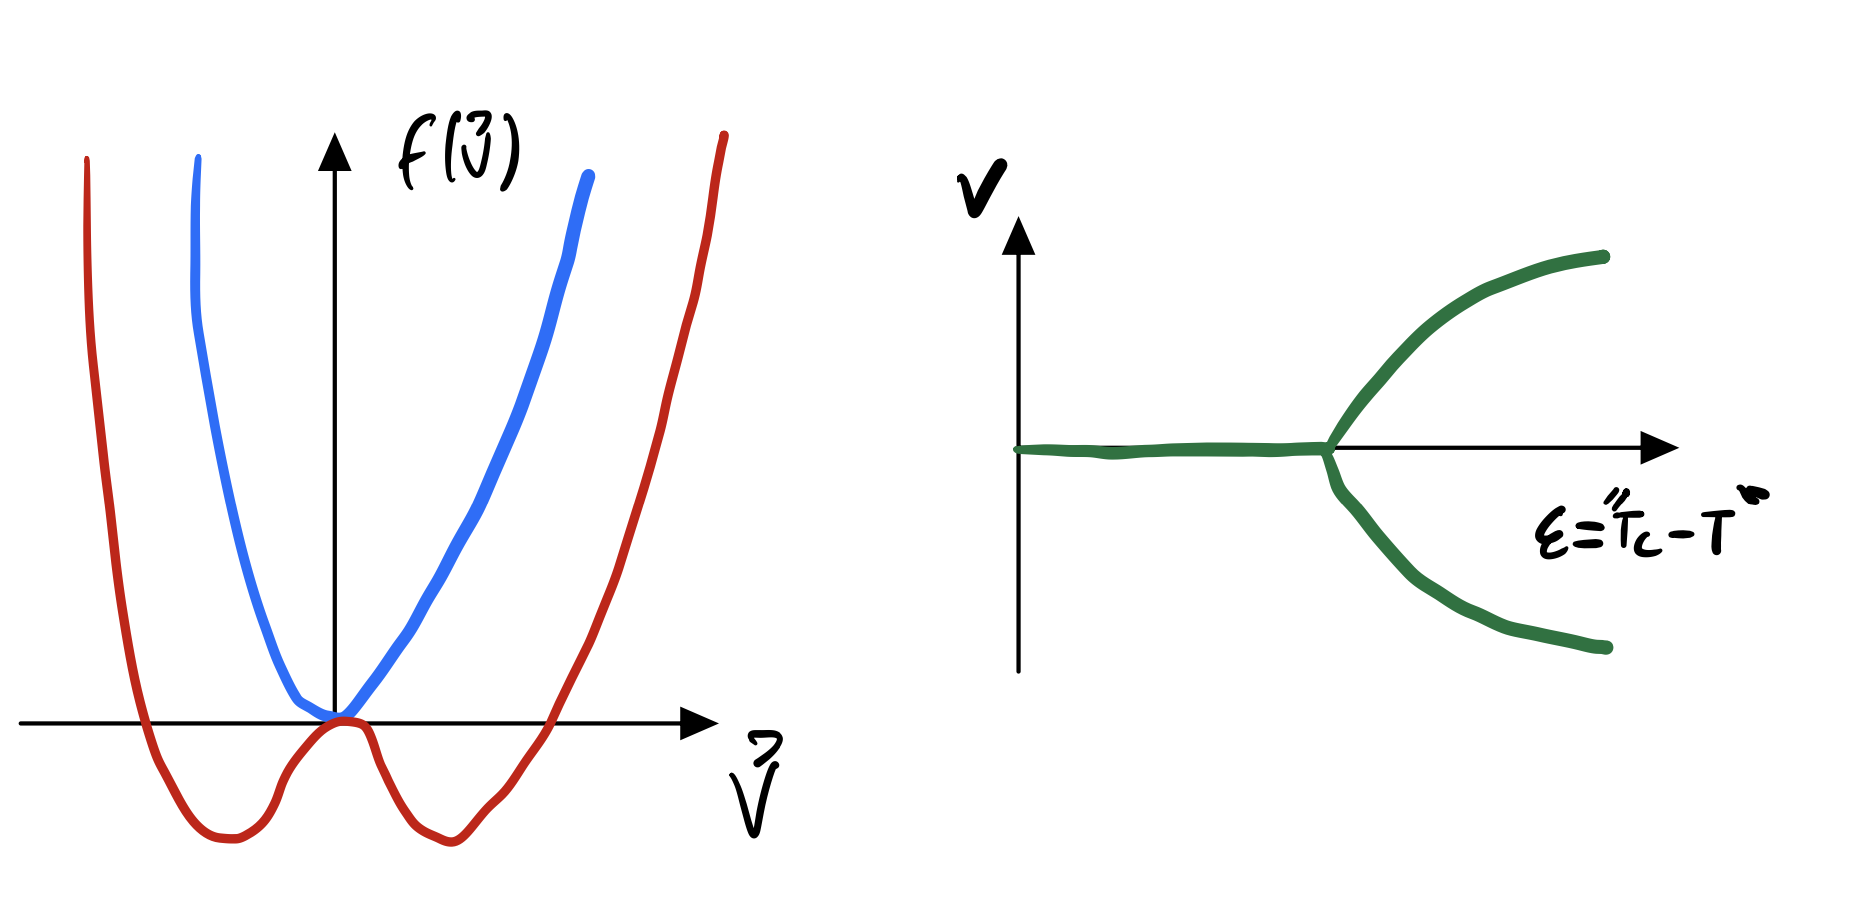
\includegraphics[scale=0.35]{Lectures/Images/lec8-bifurcation.png}
\end{center}

Where for $\e > 0$ we have pitchfork bifurcation. Much like in the magnet case, as a function of noise (temperature) we have a phase transition as detectable in the velocity (magnetization).

To account for the fluid aspects of the system, we think back to Navier-Stokes. One equation is the continuity/density conservation equation:
\begin{equation}
    \p_t \rho + \nabla \cdot (\rho\v{v}) = 0
\end{equation}
and from the other equation, we get insight on how to modify Eq. \eqref{eq:TTbifurcationterms} - we add pressure and viscosity terms on the RHS, as well as the convective term on the LHS:
\begin{equation}
    \boxed{\rho\left[\p_t \v{v} + \lambda_1(\v{v} \cdot \nabla)\v{v}\right] = -\nabla P + \eta \nabla^2\v{v} + \alpha \v{v} - \beta\abs{\v{v}}^2\v{v}}
\end{equation}
Note the one deviation from Navier-Stokes; there the invariance under boosts enforced $\lambda_1 = 1$, but we lose that here now that there is a preferred velocity. The above is the so-called Toner-Tu model. Minimally, it is as if we ``glue together'' pitchfork bifurcation with Navier-Stokes.
\section{Odd Viscosity}

\subsection{Motivations/Systems with Odd Viscosity}
Recall that we previously looked at crystals with non-central interactions, which were composed of colloids; but there are two phases - a crystal/solid phase as well as a fluid phase. There, we saw transverse lubrication forces.

If you did an advanced class in statistical mechanics, you may have studied kinetic theory - where you start with the microscopic theory of collisions of particles, and from this derive the distribution, hydrodynamics etc. In the context of having transverse forces, we can have parity violating collisions (this is the key!). As a function of the collision angle, we are able to derive the (odd) viscosities, in the same way that you can do the micro-to-macro derivation for regular fluids.

There are lots of examples of odd viscosity in soft matter systems, e.g. spinning embryos, colloids, rotating bacteria etc. But they also appear in quantum systems, e.g. polyatomic cold gases and graphene.

What we will do here - instead of starting from the microscopic theory and coarse graining, we will write down hydrodynamic equations from the symmetries of the problem, and study the system from there (similar to how we wrote down the stiffness tensor for odd elasticity). This doesn't tell us the dependence on the microscopic parameters, but can still tell us about the dynamics.

\subsection{Viscosity and Odd Viscosity}
We will write the stress:
\begin{equation}
    \sigma_{ij} = K_{ijkl}\p_l u_k
\end{equation}
where $\p_l u_k$ is the gradient of displacement and $K_{ijkl}$ is the stiffness tensor. But a medium can also have a viscous component to the stress; we thus add:
\begin{equation}
    \sigma_{ij} = K_{ijkl}\p_l u_k + \eta_{ijkl}\p_l \dot{u}_k
\end{equation}
where $\dot{u}_k = v_k$ is the velocity, and $\eta_{ijkl}$ is the viscosity tensor.

What we will now do - we ask if we allow for parity violation (of collisions), then what new entries appear in $\eta_{ijkl}$ compared to a normal fluid? This is very similar to the procedure we went through for looking at entries of $K_{ijkl}$ when we relaxed assumptions of symmetries. We remark that if we can write:
\begin{equation}
    K_{ijkl} = \frac{\delta^2 E}{\delta(\p_j u_i)\delta(\p_l u_k)}
\end{equation}
Then we have a conservative medium, and also clearly:
\begin{equation}
    K_{ijkl} = K_{klij}
\end{equation}
But if we have odd elasticity, then we could \emph{not} write things in this way:
\begin{equation}
    K^0_{ijkl} \neq \frac{\delta^2 E}{\delta(\p_j u_i)\delta(\p_l u_k)}
\end{equation}

What is the analog for the viscosity? Let us start by writing the power dissipated in the medium as:
\begin{equation}\label{eq:viscosity}
    P = T\dot{S} = \eta_{ijkl}v_{ij}v_{kl}
\end{equation}
where:
\begin{equation}
    v_{ij} = \p_j \dot{u}_i
\end{equation}
Much like the elasticity had the single-particle analog of moving in a harmonic potential $U = \frac{1}{2}kx^2$ and so $F = -kx$, there is also a single-particle analog here with a particle moving in a viscous fluid $P = -vf \propto \eta v^2$. So, Eq. \eqref{eq:viscosity} is equivalent to:
\begin{equation}
    E = \frac{1}{2}K_{ijkl}u_{ij}u_{kl}
\end{equation}
which odd elasticity of course breaks. The analog of that scenario is:
\begin{equation}
    \eta_{ijl} = \frac{\delta^2(T\dot{S})}{\delta(\p_j \dot{u}_i)\delta(\p_l \dot{u}_k)}
\end{equation}
and this is very much the standard notion of viscosity. But, in the same way where we gave up $E = \frac{1}{2}K_{ijkl}u_{ij}u_{kl}$, we will say:
\begin{equation}
    P \neq \eta_{ijkl}v_{ij}v_{kl}
\end{equation}
And thus that there exists an odd contribution:
\begin{equation}
    \eta^o_{ijkl} \neq \frac{\delta^2(T\dot{S})}{\delta(\p_j \dot{u}_i)\delta(\p_l \dot{u}_k)}
\end{equation}
So let us, as we did for elasticity, split the viscosity into an odd and even part:
\begin{equation}
    \eta_{ijkl} = \eta^e_{ijkl} + \eta^o_{ijkl}
\end{equation}
with $\eta^e_{ijkl}$ the familiar (even) viscosity with:
\begin{equation}
    \eta^{e}_{ijkl} = +\eta^{e}_{klij}
\end{equation}
and the new term is the odd viscosity:
\begin{equation}
    \boxed{\eta^o_{ijkl} = -\eta^o_{klij}}
\end{equation}
Now mapping $ij \to \alpha, kl \to \beta$ (recall the map we did with the elasticity tensor) we can write:
\begin{equation}
    \eta^o_{\alpha\beta} = -\eta^o_{\beta\alpha}
\end{equation}
If $\alpha, \beta$ could only take values $0, 1$ then $\eta^o_{\alpha\beta}$ would just be $\e_{\alpha\beta}$, from which we can see the chirality of the medium start to emerge. Here, we are taking the $ijkl$ that can take on 2 values to $\alpha, \beta$ that can take on 4 values.

Like the odd elastodynamic equations knew about the odd elasticisty (even though the energy didn't!), similarly here there should be odd fluid dynamic equations that know about the odd viscosity (even though the power seems to not ``know'' about it, as it is not derived variationally). We will accordingly modify the Navier-Stokes equations.

\subsection{Navier-Stokes Equation}
We fluid analog of $ma = F$ is:
\begin{equation}
    \rho D_t v_i = \p_j \sigma_{ij} + f_i
\end{equation}
Here, we have the divergence of the flux of linear momentum $\p_j \sigma_{ij}$ and $\rho D_t v_i$ is the time derivative of the density of linear momentum. $f_i$ is an external body force, e.g. gravity with $g\rho$, or the Coriolis force, or the Lorentz force etc. (c.f. $\p_j \sigma_{ij}$ we can think about as surface forces). Note that the $D_t$ above has two pieces, because there is both an explicit and implict time dependence through the coordinates:
\begin{equation}
    D_t = \p_t + \dpd{x_i}{t}\dpd{}{x_i} = \p_t  + v_k\p_k
\end{equation}
this is also known as a convective derivative. This introduces an interesting feature, because now the equation is nonlinear in $v$. In the regime where this is important (the high Reynolds number regime), all of the physics of chaotic systems affects fluid systems, and deep in that regime we have turbulence (and we will study what happens in this regime when we add odd visocity). 

Further complicating things, $\sigma_{ij}$ also has two pieces:
\begin{equation}
    \sigma_{ij} = \sigma_{ij}^h + \eta_{ijkl}\p_l v_k
\end{equation}
where:
\begin{equation}
    \sigma_{ij}^h = -p\delta_{ij}
\end{equation}
comes from the hydrostatic pressure, and $\eta_{ijkl}\p_l v_k$ are the viscous stresses, which generates the force:
\begin{equation}
    f_i^{\text{vis}} = \eta \Delta v_i = \eta \nabla^2 v_i
\end{equation}
Hence, we can write out:
\begin{equation}
    \rho(\p_t v_i + v_k\p_k v_i) = -\nabla p + \eta \nabla^2 v_i + f_i
\end{equation}
Here, we assume that the $\eta$ comes from shear viscosity, wherein the incompressibility condition:
\begin{equation}
    \nabla \cdot \v{v} = 0
\end{equation}
tells us that there is no bulk viscosity contribution.

Now, if we allow for odd viscosity, we should generate new terms in the above equation of motion, much in the same way that odd elasticity generated terms in the equation beyond the shear and bulk moduli. Put another way, we have ignored the possibility of terms:
\begin{equation}
    \eta^o_{ijkl} = \frac{\eta_{ijkl} - \eta_{klij}}{2}
\end{equation}
and the impact they would have on the above Navier-Stokes equation.

\subsection{Modifying Navier-Stokes}
To make things concrete, let us study first two dimensional simple fluids with odd viscosity. We write the matrix equation:
\begin{equation}
    \sigma_\alpha = \eta_{\alpha\beta}\sigma_\beta
\end{equation}
with:
\begin{center}
    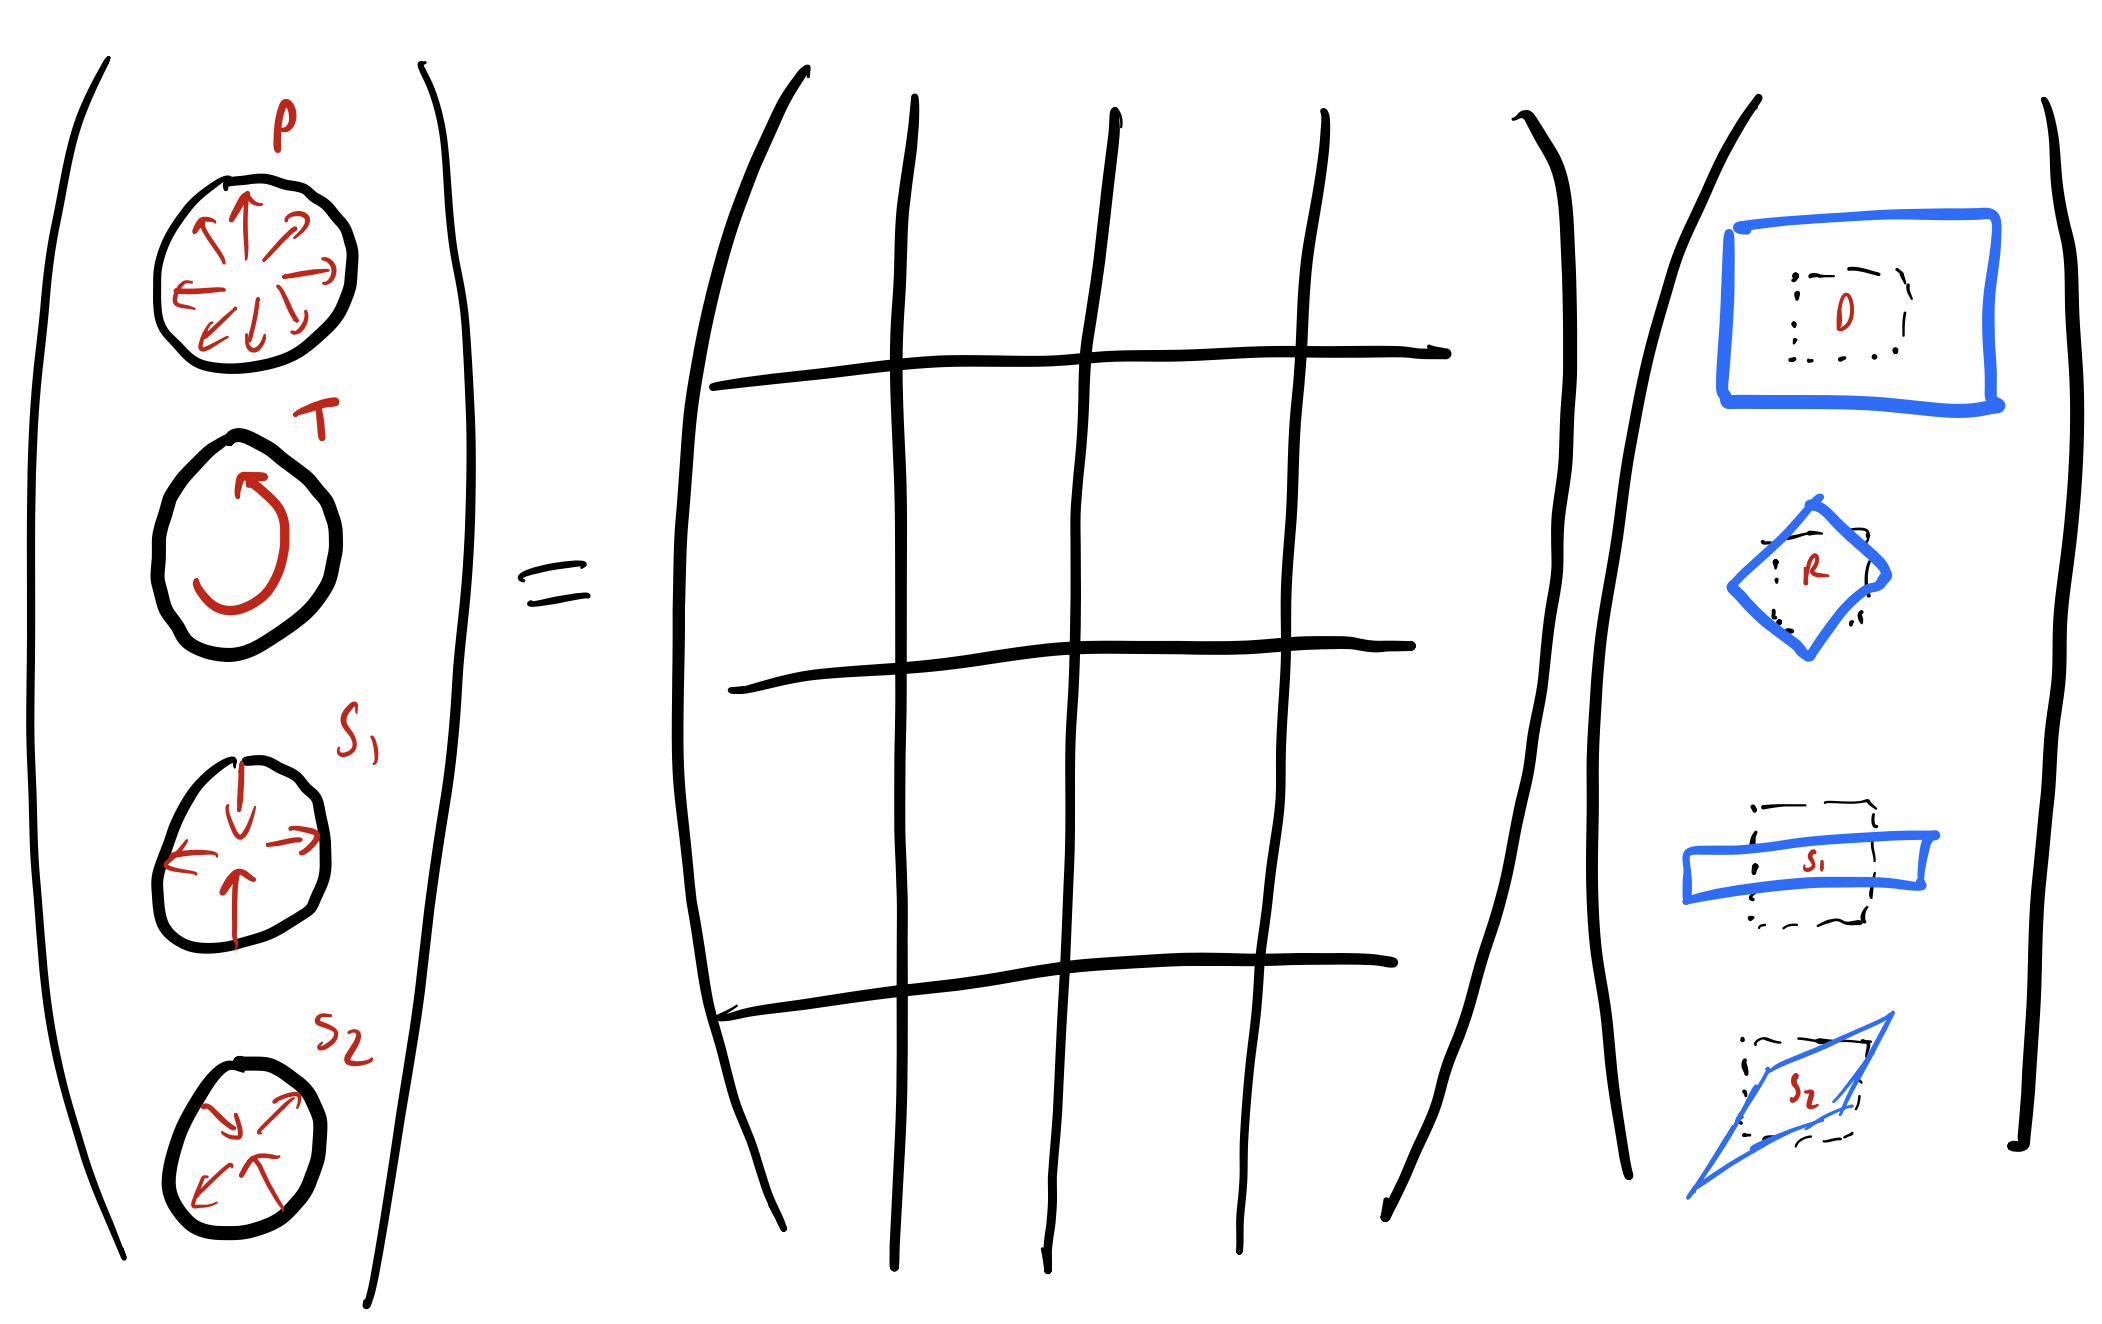
\includegraphics[scale=0.3]{Lectures/Images/lec2-stiffnessmatrix.png}
\end{center}
\begin{equation}
    \m{\text{P} \\ \text{T} \\ \text{SS1} \\ \text{SS2}} = \m{\cdot & \cdot & \cdot & \cdot \\ \cdot & \cdot & \cdot & \cdot \\ \cdot & \cdot & \cdot & \cdot \\ \cdot & \cdot & \cdot & \cdot}\m{\text{D} \\ \text{R} \\ \text{S1} \\ \text{S2}}
\end{equation}
This is really a statement about taking the stresses/strains and projecting on the group of matrices:
\begin{equation}
    \tau^0 = \m{1 & 0 \\ 0 & 1}, \quad \tau^1 = \m{0 & 1 \\ -1 & 0}, \quad \tau^2 = \m{1 & 0 \\ 0 & -1}, \quad \tau^3 = \m{0 & 1 \\ 1 & 0}
\end{equation}
where with this projection:
\begin{equation}
    \sigma^\alpha = \tau^\alpha_{ij}\sigma_{ij}
\end{equation}
\begin{equation}
    v^\beta = \tau_{ij}^\beta v_{ij}
\end{equation}
\begin{equation}
    \eta^{\alpha\beta} = \frac{1}{2}\tau^{\alpha}_{ij}K_{ijkl}\tau^\beta_{kl}
\end{equation}
Let us populate the entries of the matrix:
\begin{equation}
    \m{\text{P} \\ \text{T} \\ \text{SS1} \\ \text{SS2}} = \m{\xi & \cdot & 0 & 0 \\ \cdot & \cdot & 0 & 0 \\ 0 & 0 & \eta & \cdot \\ 0 & 0 & \cdot & \eta}\m{\text{D} \\ \text{R} \\ \text{S1} \\ \text{S2}}
\end{equation}
$\xi$ is the bulk viscosity, $\eta$ is the shear viscosity. The off diagonal blocks are assuming isotropy because we cannot connect the scalar and bivector parts. Further, the form of the rotation operator enforces the off diagonals to be zero (as the rotation operator forces that the odd diagonals are equal and opposite, and the symmetry of the matrix enforces that they are equal - hence they must be zero). So:
\begin{equation}
    \m{\text{P} \\ \text{T} \\ \text{SS1} \\ \text{SS2}} = \m{\xi & 0 & 0 & 0 \\ 0 & 0 & 0 & 0 \\ 0 & 0 & \eta & 0 \\ 0 & 0 & 0 & \eta}\m{\text{D} \\ \text{R} \\ \text{S1} \\ \text{S2}}
\end{equation}
If we now relax the $\eta_{\alpha\beta} = \eta_{\beta\alpha}$ condition so the matrix is not symmetric, in the lower diagonal block and upper diagonal block we can introduce new terms, as well as a rotation term:
\begin{equation}
    \m{\text{P} \\ \text{T} \\ \text{SS1} \\ \text{SS2}} = \m{\xi & \eta^B & 0 & 0 \\ \eta^A & \eta^R & 0 & 0 \\ 0 & 0 & \eta & \eta^0 \\ 0 & 0 & -\eta^0 & \eta}\m{\text{D} \\ \text{R} \\ \text{S1} \\ \text{S2}}
\end{equation}
Rotational invariance would set $\eta^B = \eta^R = 0$, but even with this assumption $\eta^A$ would persist. What remains is completely analogous to the $A, K^0$ coefficients that arose in our discussion of odd elasticity.

The interpretation of $\eta^A$ is depending on the rate at which you can compress, there is a torque in response. If you know that your fluid has zero torque density, then it vanishes. The odd elasticity equivalent was the robots with a bond-bending angle, which had $K^0$ but no $A$. $\eta_As$ can only exist if $\sigma_{ij} \neq \sigma_{ji}$.

\subsection{Equations - Tensorial Form}
Instead of writing things in this intuitive notation, we can also write things down in tensorial notation (like we did for $K_{ijl}$), which is generally more useful for calculations. Let us write:
\begin{equation}
    \eta_{ijkl} = \xi \delta_{ij}\delta_{kl} - \eta^A \e_{ij}\delta_{mn} - \eta^B \delta_{ij}\e_{kl} + \eta^R \e_{ij}\e_{kl} + \eta(\delta_{il}\delta_{jk} + \delta_{ik}\delta_{jl} - \delta_{ij}\delta_{kl}) + \eta^0\frac{1}{2}(\e_{ik}\delta_{jl} + \e_{il}\delta_{jk} + \e_{jk}\delta_{il} + \e_{jl}\delta_{ik})
\end{equation}
The latter two look complicated, but you can check that $\eta_{ijkl} = \eta_{klij}$ for the even term and $\eta_{ijkl} = -\eta_{klij}$ for the odd term.

If we were to add a pressure or pre-torque through $\sigma^h$, the above is modified to be:
\begin{equation}
        \m{\text{P} \\ \text{T} \\ \text{SS1} \\ \text{SS2}} = \m{\xi & \eta^B & 0 & 0 \\ \eta^A & \eta^R & 0 & 0 \\ 0 & 0 & \eta & \eta^0 \\ 0 & 0 & -\eta^0 & \eta}\m{\text{D} \\ \text{R} \\ \text{S1} \\ \text{S2}} + \m{-p \\ -\tau \\ 0 \\ 0}
\end{equation}
Now, taking this definition of $\sigma_{ij}$, we can put it into the Navier-Stokes equation:
\begin{equation}
    \rho D_t \v{v} = \underbrace{\nabla \sigma^h}_{=0} + \xi\nabla(\nabla \cdot \v{v}) + \underbrace{\eta\nabla^2\v{v}}_{\eta\p_k \p_k v_i} + \underbrace{\eta^0\e \cdot \nabla^2 \v{v}}_{\eta^0\e_{ij}\p_k\p_k v_j} - \eta^A \e \cdot\nabla(\nabla \cdot \v{v}) + \eta^B \nabla(\nabla \times \v{v}) - \eta^R \e \cdot \nabla(\nabla \times \v{v})
\end{equation}
Next time, we remove some terms, and study a fluid with just $\eta, \eta^0$ terms in 2-D. We then progress to more complicated settings of 3-D and fluids with turbulence.
\section{Odd Viscosity II}

\subsection{Summary of Last Lecture}
Last time, we explored (in quite a bit of detail) odd viscosity. If we have a linear constitutive equation:
\begin{equation}
    \sigma_{ij} = \eta_{ijkl}v_{kl}
\end{equation}
If this viscosity is derived from entropy production/dissipation $T\dot{S}$, then it must be case that the viscosity tensor is symmetric:
\begin{equation}
    \eta_{ijkl} = \eta_{klij}
\end{equation}
but if we relax this assumption, we can have an odd component:
\begin{equation}
    \eta_{ijkl} = \eta^e_{ijkl} + \eta^o_{ijkl}
\end{equation}
Where the odd part is, as the name suggests, odd under interchange:
\begin{equation}
    \eta^o_{ijkl} = -\eta^o_{klij}
\end{equation}
Note that this part of the tensor cannot be associated with power dissipation. To see this:
\begin{equation}
    P = \eta^o_{ijkl}v_{ij}v_{kl} = \eta^o_{ijkl}v_{kl}v_{ij} = -\eta^o_{klij}v_{kl}v_{ij} = -\eta^o_{ijkl}v_{ij}v_{kl} \implies P = 0
\end{equation}
So, we can see that odd viscosity does not contribute to dissipation, but does contribute to the equation of motion:
\begin{equation}
    \underbrace{D_t v_i}_{\p_t v_i + v_k \p_k v_i} = \p_j \sigma_{ij} + f^{\text{ext}}
\end{equation}
which expanding:
\begin{equation}\label{eq:modNavierStokes}
    \rho D_t v_i = -\p_i p + \eta \Delta v_i + \eta^0\e_{ij}v_j
\end{equation}
possibly supplemented by $\nabla \cdot \v{v} = 0$ if the fluid is incompressible. We can interpret what we have done above as a completion of the Navier-Stokes equation with a chiral term.

\subsection{Odd Viscosity as Pressure}
If we take the above equation and define a new pressure term:
\begin{equation}
    p' = p - \eta^0\omega
\end{equation}
with $\omega$ the vorticity, then we can write:
\begin{equation}
    \rho D_t v_i = -\p_i p' + \eta \Delta v_i
\end{equation}
So the odd viscosity can be reabsorbed into the pressure! Hence we could measure it by measuring the pressure. But if we solved this on a computer, the flow would not change - just a Lagrange multiplier. Hence we call the odd viscosity term a boundary term. Note that the odd viscosity being nothing more than a renormalization of the pressure term is only true if the fluid is incompressible.

The vorticity is the curl of the velocity field:
\begin{equation}
    \gv{\omega} = \nabla \times \v{v}
\end{equation}
or in two dimensions:
\begin{equation}
    \omega = \e_{ij}\p_i v_j = \p_x v_y - \p_y v_x
\end{equation}
Now looking at:
\begin{equation}
    \p_i \omega = \m{\p_x(\p_x v_y - \p_y v_x) \\ \p_y(\p_x v_y - \p_y v_x)}
\end{equation}
The incompressibility condition tells us that:
\begin{equation}
    \p_x v_x + \p_y v_y = 0 \implies \p_x v_x = -\p_y v_y
\end{equation}
Now rewriting the gradient of the vorticity (by commuting the partials):
\begin{equation}
    \p_i \omega = \m{\p_x^2 v_y - \p_y \p_x v_x  \\ \p_x \p_y v_y - \p_y^2 v_x} = \m{\p_x^2 v_y - \p_y (-p_y v_y) \\ \p_x (-\p_x v_x) - \p_y^2 v_x} = \m{(\p_x^2 + \p_y^2)v_y \\ (\p_x^2 + \p_y^2)(-v_x)} = \nabla^2 \m{v_y \\ -v_x} = \m{0 & -1 \\ 1 & 0}\nabla^2\v{v} =  \e_{ij}\Delta v_j
\end{equation}
Hence:
\begin{equation}
    -\p_i p' = -\p_i p + \eta^0 \p_i \omega = -\p_i p + \eta^0 \e_{ij}\Delta v_j
\end{equation}
And so we have successfully repackaged the odd viscosity term into the pressure (under the assumptions that we are in 2-D and the fluid is incompressible!)

\subsection{Simple example: Pressure difference due to odd viscosity}
Experiment (actually realized) - imagine two plates, and a fluid with odd viscosity flowing in between. We apply a pressure gradient $\p_x P = G$. We assume there is a no slip boundary condition. Everything looks symmetric - we have a symmetric laminar flow profile. But, we will find that we can measure a pressure differential between the two plates.

\begin{center}
    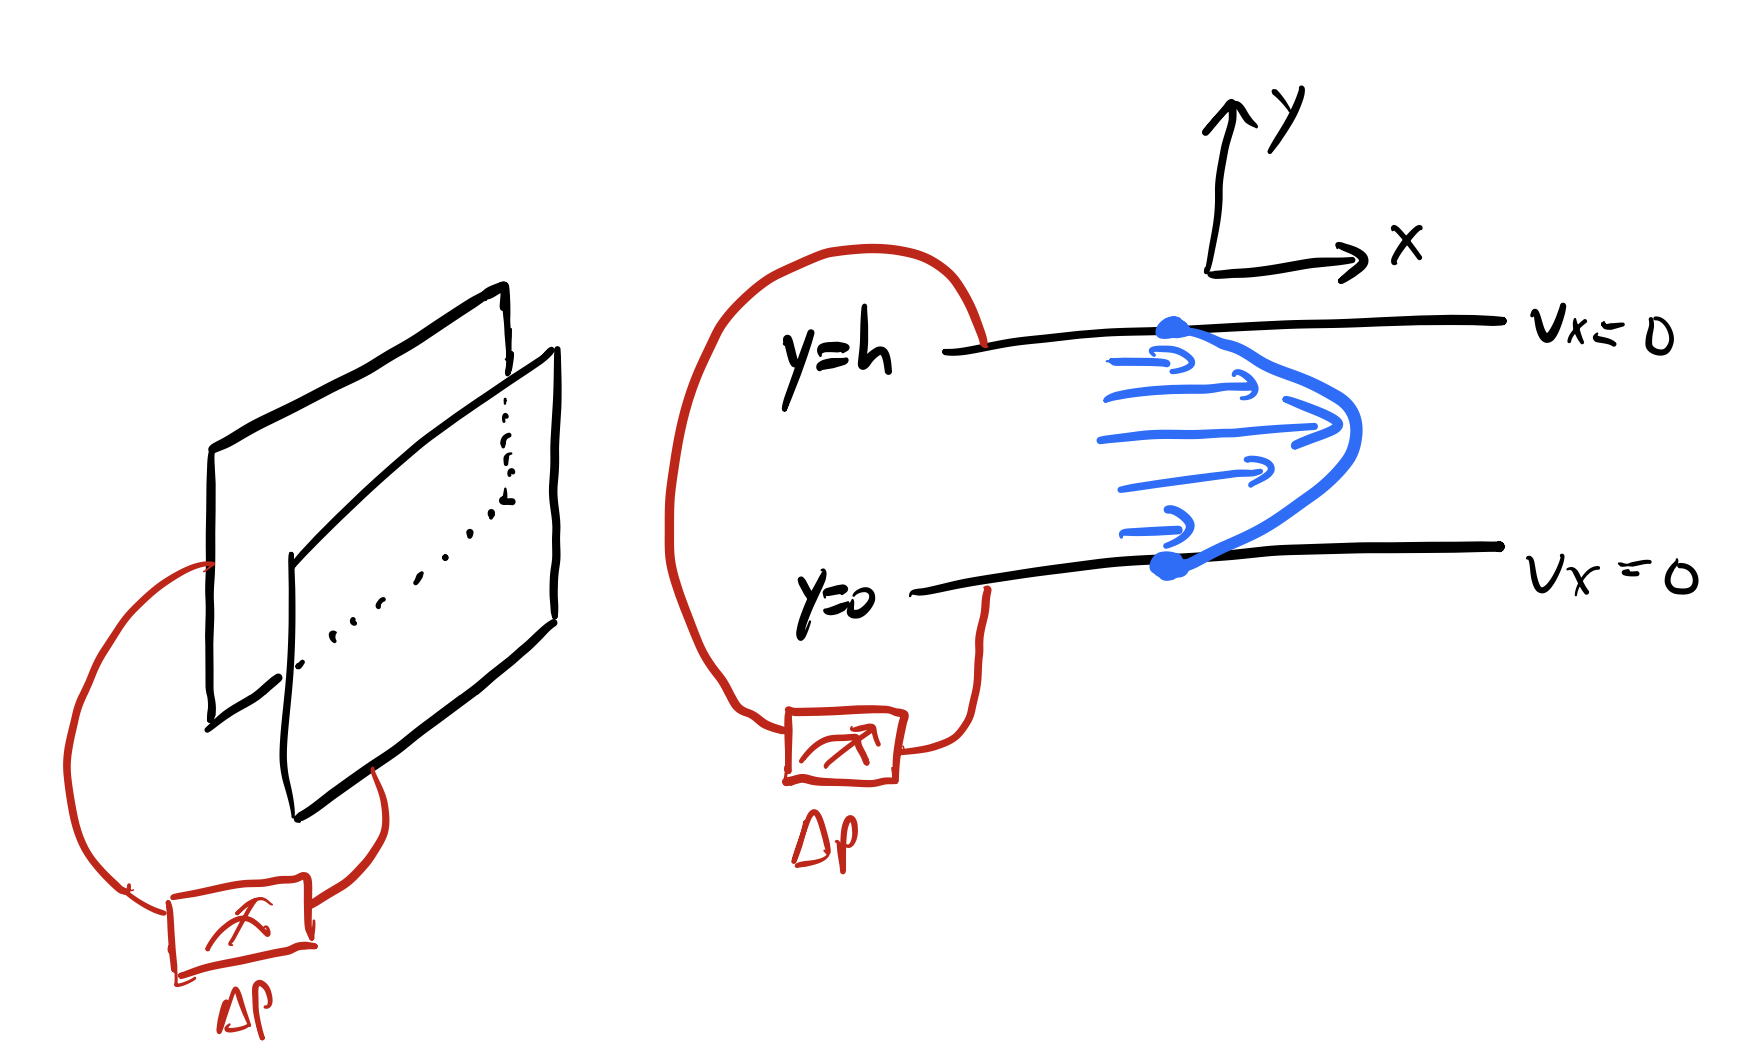
\includegraphics[scale=0.35]{Lectures/Images/lec10-pressuredifferential.png}
\end{center}

Note: When the Reynolds number is low, the $\rho D_t v_i$ term (which $\text{Re}$ multiplies) can be neglected, and then solving for the hydrodynamics reduces to:
\begin{equation}
    \eta\Delta v_i = \p_i p'
\end{equation}
Which is just the Laplace equation with a source term - this is one of the most well-solved problems in the universe; we have the solution:
\begin{equation}
    \v{v} = \frac{G}{2\eta}y(h-y)\xhat
\end{equation}
I.e. the flow looks like a parabola. This flow is unchanged by the addition of the odd viscosity term, because the solution only depends on the gradient in the x-direction.

Calculating the vorticity:
\begin{equation}
    \omega = \p_x v_y - \p_y v_x = \p_x(0) - \p_y\left(\frac{G}{2\eta}y(h-y)\right) = -\frac{G}{2\eta}(h - 2y)
\end{equation}

Now, we want to evaluate (using $p' = p - \eta^0 \omega$) the pressure differential:
\begin{equation}
    \Delta p = p(y=h) - p(y=0) = Gh\frac{\eta^0}{\eta}
\end{equation}
This is a measurable quantity, and this was measured in the 70s/80s in Linden.

\subsection{Compressible Systems}
What happens now if our fluid is compressible - e.g. we consider a gas flowing in a channel? What happens if we assume the nonlinear terms cannot be neglected?

To this end, we want to try to rewrite the the equation for the velocity field to get an equation for the vorticity. Multiplying Eq. \eqref{eq:modNavierStokes} by $\e_{li}\p_l$ (i.e. taking a curl of the equation) and defining the kinematic viscosity $\nu = \frac{\eta}{\rho}$ and $\nu^0 = \frac{\eta^0}{\rho}$ we find:
\begin{equation}
    \p_t \omega + \nabla \cdot (\omega \v{v}) = \nu \nabla^2 \omega + \nu^0\nabla^2(\nabla \cdot \v{v})
\end{equation}
Where the curl of the gradient of the pressure drops out, and the last term was obtained from:
\begin{equation}
    \e_{li}\p_l \e_{ij}\p_k\p_k v_j = \delta_{lj}\p_l \p_k \p_k v_j = \nabla^2 (\nabla \cdot \v{v})
\end{equation}
Note that the last term cooberates our story that if the fluid is incompressible then the odd viscosity term drops out of the viscosity. The odd viscosity acts as an additional source of vorticity which is proportional to the divergence of the velocity.


If we look at the pressure term in the Navier-Stokes equation:
\begin{equation}
    \frac{1}{\rho}\p_x p = \frac{1}{\rho}\dpd{p}{\rho}\dpd{\rho}{x}
\end{equation}
when $c < v$, i.e. the velocity is larger than the speed of sound in the fluid, then we can cause shock waves, and mathematically we can neglect the $\dpd{p}{\rho}\dpd{\rho}{x}$ term which is of order $c$. Therein the Navier-Stokes equation becomes:
\begin{equation}
    \boxed{\p_t v_x + v_x \p_x v_x = \nu \p_x^2 v_x}
\end{equation}
Which is an equation with both dissipation and nonlinearity, known as the \emph{Burges equation}. What he found was that the above equation can have stable solutions. This is surprising, because nonlinearities cause waves to break generically (experimentally confirm this by watching the sea by sipping a cocktail). But the diffusive/dissipative term allows for the stabilization of the nonlinearity. Though it does not appear in the above, another option would be to add dispersion (which leads to higher order equations - relevant for shallow water, for example). The stable solutions look like shock waves:

\begin{center}
    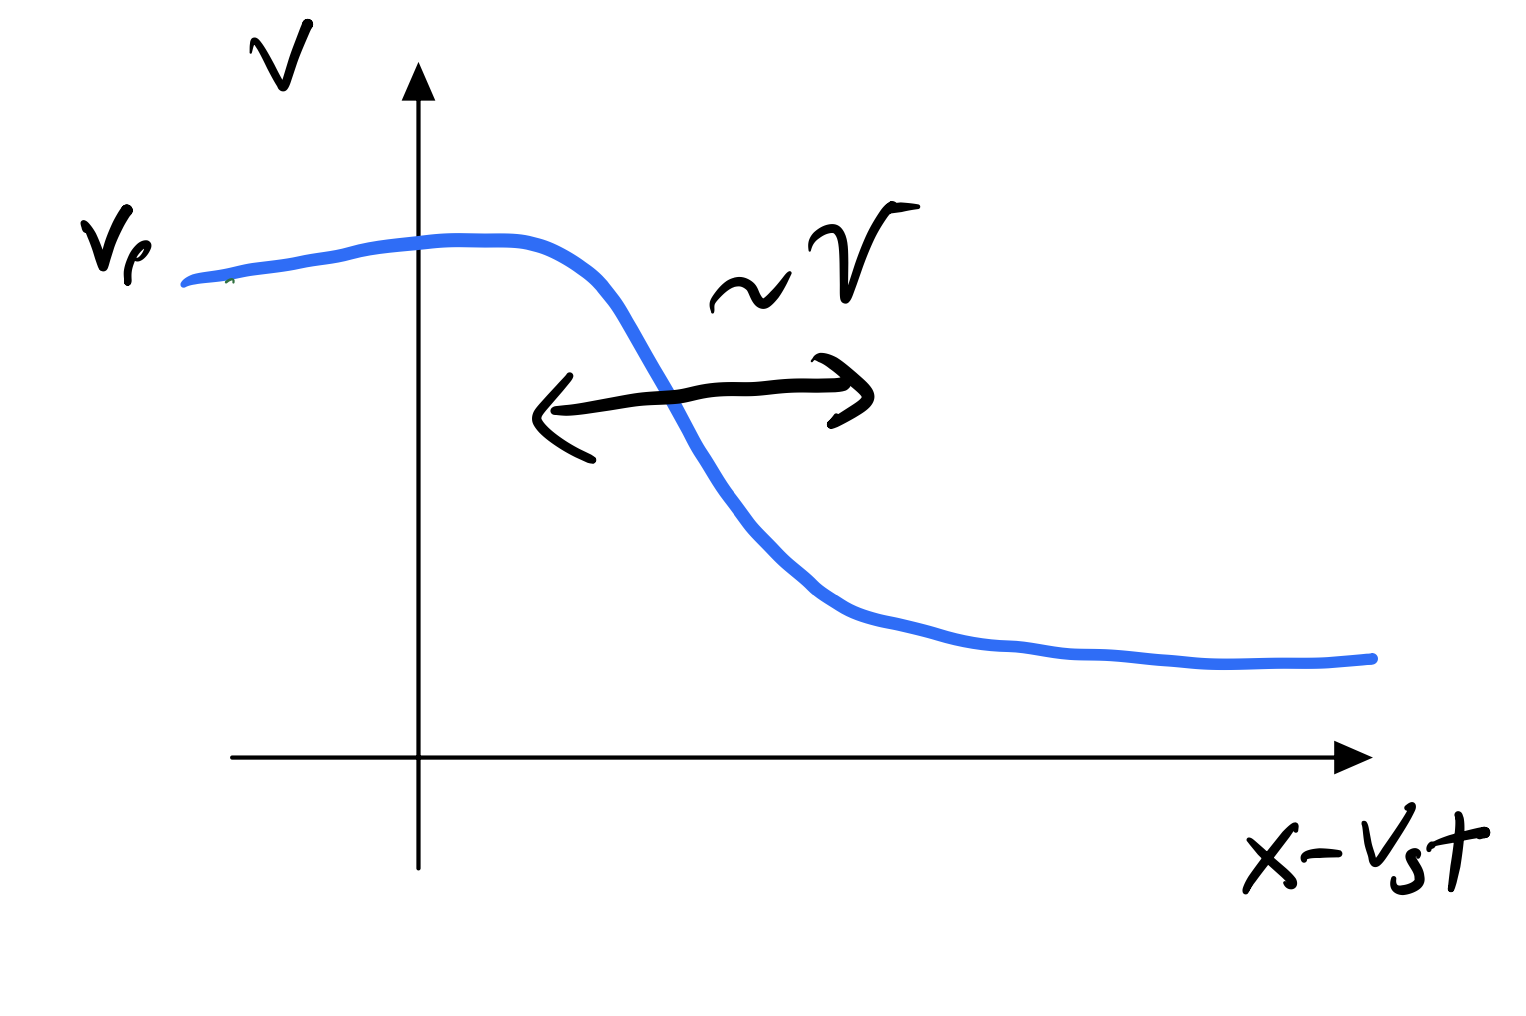
\includegraphics[scale=0.35]{Lectures/Images/lec10-shockwave.png}
\end{center}

Wherein we have a shock wave, caused by, for example, a piston moving with speed $v_p$, causing a shock wave travelling with speed $v_s$ and with width profile $\omega \sim \nu$. What happens if we calculate the divergence of the velocity? Behind and in front of the travelling shockwave wavefront, the divergence vanish. There is high concentration of divergence of velocity at the shock wavefront itself. If we now allow for flow in two dimensions, this divergence can be a source for the vorticity (we require 2D as $\omega$ is the curl of the velocity field).

You might have asked - should we not have calculated the correction to the Burges equation due to the odd viscosity. Really, we should consider:
\begin{equation}
    v_x = (\text{zeroth order}) + \frac{\eta_0}{\eta}(...)
\end{equation}
\begin{equation}
    v_y = \frac{\eta_0}{\eta}(...)
\end{equation}
The play is to calculate the zeroth order $v_x$ term, then plug things back in to calculate the first order corrections, and so on\dots But we could also be interested in the $\frac{\eta_0}{\eta} \gg 1$ limit. What happens here? Well, this corresponds to the large-odd viscosity limit. This leads to an oscillatory part/ringing of the waveform superimposed on top of the shock wave:

\begin{center}
    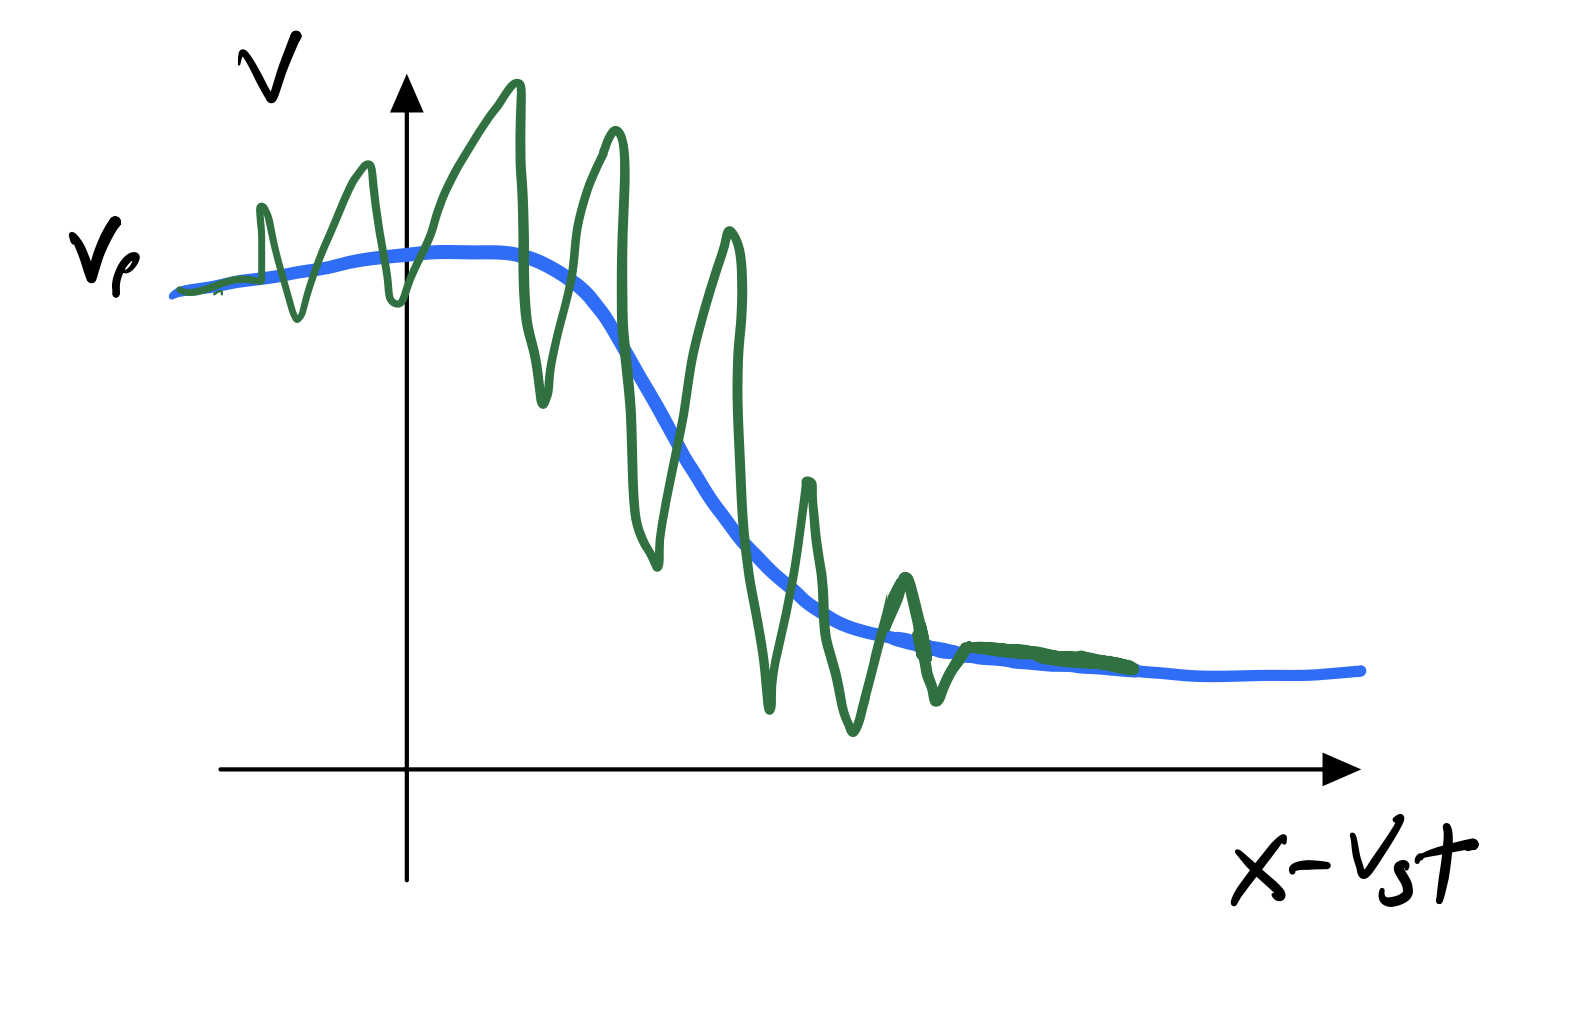
\includegraphics[scale=0.35]{Lectures/Images/lec10-ringing.png}
\end{center}

Next week, we start to discuss turbulence.
\section{Turbulence}

\subsection{Overview of Lecture}
Today we will study turbulence - we will first review the idea of a Reynold's number. Then, we will look at the dynamics of turbulence, and see how it is modified in the presence/addition of chiral terms.

The equation we consider is:
\begin{equation}
    \rho[\p_t v_i + v_k \p_k v_i] = - \nabla_i p + \eta \nabla^2 v_i + \eta^0 (\hat{\v{z}} \times \nabla^2 \v{v})_i
\end{equation}
As well as the incompressability condition $\nabla \cdot \v{v} = 0$. Dividing out by $\rho$ we call $\frac{\eta}{\rho} = \nu$ and $\frac{\eta^0}{\rho} = \nu^0$, and so:
\begin{equation}
    \p_t v_i + v_k \p_k v_i = - \frac{1}{\rho}\nabla_i p + \nu \nabla^2 v_i + \nu^0 (\hat{\v{z}} \times \nabla^2 \v{v})_i
\end{equation}
The last term is the 3D generalization of what we wrote down last time, $\eta^0\e_{ij}\p_i \nabla^2v_j$. A key observation - in 3D we no longer have isotropy, because the axis of rotation points in some direction in space (c.f. 2D where the rotation axis can be chosen to point out of the plane). We remark that in 3D, the $\nu^0 (\hat{\v{z}} \times \nabla^2 \v{v})_i$ is not the only term we can have. This is a bit of a stylized/simplified theory, but let us study it and ignore the other possible terms (which do have similar character, e.g. in that they are chiral).

Let us study turbulence as it was understood by Kolmogorov, then see how this $\nu^0 (\hat{\v{z}} \times \nabla^2 \v{v})_i$ term modifies his predictions.

\subsection{Reynold's Number}
It is often to consider equations in dimensionless units; if we measure speed as $\frac{v}{V} = \tilde{v}$ and $\frac{r}{L} = \tilde{r}$ then we can have a dimensionless casting of time as $\frac{t}{\frac{L}{V}} = \tilde{t}$. With this, we define the dimensionless parameter - the \emph{Reynold's Number}:
\begin{equation}
    \text{Re} = \frac{VL}{\nu}
\end{equation}
We want to write down Navier-Stokes in terms of dimensionless parameters as:
\begin{equation}
    \text{Re}\left[\dpd{\tilde{\v{v}}}{\tilde{t}} + (\tilde{\v{v}}\cdot\tilde{\nabla})\tilde{\v{v}}\right] = -\tilde{\nabla}\tilde{p} + \tilde{\nabla}^2\tilde{\v{v}}
\end{equation}
How do we get this? We can write the $\nu$ term as:
\begin{equation}
    \nu\nabla^2 \v{v} = \nu \tilde{\nabla}^2\tilde{\v{v}}\frac{V}{L^2}
\end{equation}
Dividing both sides by $\nu VL^2$ and doing the same rewriting in terms of dimensionless quantities, we get:
\begin{equation}
    \dpd{\v{v}}{t} \to \frac{1}{\nu \frac{V}{L^2}}\frac{1}{\frac{L}{V}}V \dpd{\tilde{\v{v}}}{\tilde{t}} = \frac{VL}{\nu}\dpd{\tilde{\v{v}}}{\tilde{t}} = \text{Re}\dpd{\tilde{\v{v}}}{\tilde{t}}
\end{equation}

There are three limits we consider:
\begin{itemize}
    \item Kolmogorov standard turbulence: $\text{Re} \gg 1$ and $\frac{\eta^0}{\eta} = 0$
    \item Tali will show in guest lecture: $\text{Re} \ll 1$ and $\frac{\eta^0}{\eta} \gg 1$
    \item Odd turbulence: $\text{Re} \gg 1$ and $\frac{\eta^0}{\eta} \gg 1$
\end{itemize}

When $\text{Re} \gg 1$, the $\dpd{\tilde{\v{v}}}{\tilde{t}} + (\tilde{\v{v}}\cdot\tilde{\nabla})\tilde{\v{v}}$ terms are dominant. When $\text{Re} \ll 1$, the $-\tilde{\nabla}\tilde{p} + \tilde{\nabla}^2\tilde{\v{v}}$ are dominant. In the odd turbulent regime, we have that both nonlinearity and chirality ($\nu^0 (\hat{\v{z}} \times \nabla^2 \v{v})$) dominate.



\subsection{Power Spectrum}
The great genius of Kolmogorov starts with a single observation - namely that turbulence should be viewed as a statistical mechanics problem. This is not obvious as Navier-Stokes is determinisitc. But when you have strong non-linearities, an infinitesimally different initial condition can lead to a vastly different outcome. For example with fluid flowing across a sphere, at low Reynolds number (linear) you have smooth flow, while at high velocity (non-linear) you have vortices emerging:

\begin{center}
    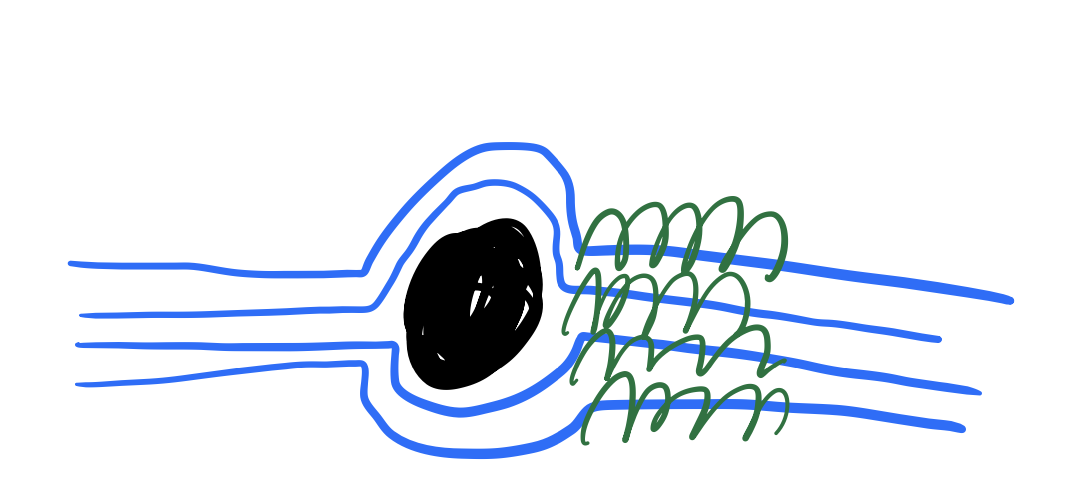
\includegraphics[scale=0.35]{Lectures/Images/lec11-fluidsphere.png}
\end{center}

We consider the power spectrum, a quantity relevant for both theorists and experimentalists. If we assume isotropic, homogenous, and fully developed turbulence:
\begin{equation}
    \v{v}(\v{x}, t) = \left(\frac{2\pi}{L}\right)^3\sum_{\v{k}}\tilde{\v{v}}(k, t)e^{i\v{k} \cdot \v{x}}
\end{equation}
With $\v{k} = (k_x, k_y, k_z) = \frac{2\pi}{L}(n_x, n_y, n_z)$. To find the average of a given observable $A$:
\begin{equation}
    \avg{A}_c = \frac{1}{L^3}\int d^3\v{x}A
\end{equation}
What we will consider is the average of $\frac{v^2}{2}$, the kinetic energy per unit mass. We can compute the average using Parseval's theorem:
\begin{equation}
    \avg{\frac{v^2}{2}}_c = \int d^3\v{k}\frac{1}{2}\abs{\tilde{\v{v}}(k, t)}^2 \equiv \int_0^\infty dk E(k, t)
\end{equation}
The fact that it is homogenous we have already used to going to $k$-space. Isotropy comes in in that in $k$-space there is no preferred direction. Hence we can write:
\begin{equation}
    \int d^3\v{k} = \int 4\pi k^2 dk
\end{equation}
So then the power spectrum (which tells us how the energy is distributes as a function of $k$):
\begin{equation}
    E(k, t) = 4\pi k^2 \frac{1}{2}\abs{\tilde{\v{v}}(k, t)}^2 = 2\pi k^2\abs{\tilde{\v{v}}(k, t)}^2
\end{equation}
If at some time we reach a steady state, then the time-dependence of $E(k, t)$ drops out. Note that the time-invariance we consider here is in a statistical sense; not that the system looks the same at all time, but the average does.

\begin{center}
    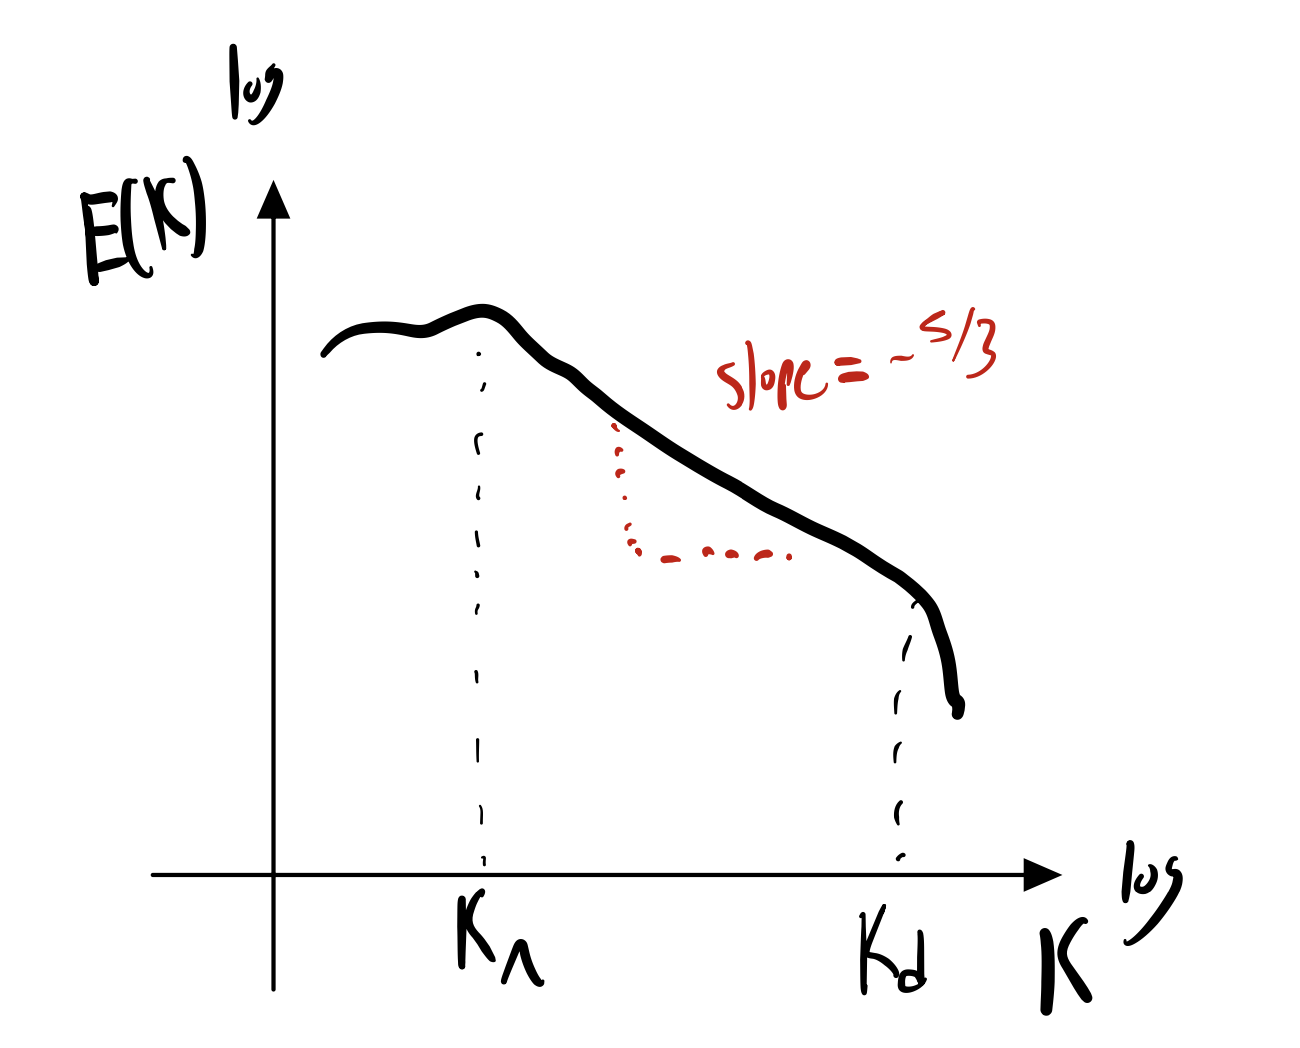
\includegraphics[scale=0.35]{Lectures/Images/lec11-spectrum.png}
\end{center}

Before it was worked out by Kolmogorov, plots/measurements existed that suggested that regimes where $E(k, t)$ becomes time-translation invariant + displays a power law. We can imagine that an experimentalist could measure; to carefully extract the power law, we need to measure something on the length scale of many many decades. We can also use astrophysical/astronomical data to measure this spectrum (albeit with some difficulty, given things like Coriolis effect breaking isotropy). Kolmogorov proved that the slope on this log-log is $-\frac{5}{3}$ under the isotropic, homogenous, fully developed assumption.

\subsection{Power Law Scaling from Vortices and Dimensional Analysis}

In the high Reynolds number scale, interesting things happen - pressure drops out, but so does the second derivative term; we lose dissipation! We consider a vortex/an eddy (we may not be able to see it physically in all systems). We could consider that some external force could be applying a perturbation at a given wavelength. We consider this lengthscale to be $L$/the system size. Since Navier Stokes is energy conserving in the $\text{Re} = \frac{VL}{\nu} \gg 1$ limit, what can happen? Energy cannot go in our out, but energy can redistribute itself, but the eddies can split into eddies of length scale $L$'. But, if it is indeed the case that $\text{Re} = \frac{VL'}{\nu} \gg 1$ even with the new eddies, then these can also potentially split and become smaller vortices. And if the condition still holds then the eddies can continue to split into eddies of $L'', L'''$ and so on. But as the length scale lowers, there may come a point where the size of the vortices/characteristic wavevector becomes such that $\text{Re} = \frac{VL^{(n)}}{\nu} \sim 1$. We call this length scale $L_d$, as it is at this length scale we can start to observe dissipation. It turns out that this self-similar process of splitting of vortices that leads to a power law. In the $E(k)$ plot we had above, the $K_\Lambda = \frac{1}{L}$ corresponding to wavevector of the system size, then we can keep splitting until we reach $K_d = \frac{1}{L_d}$ corresponding to wavevector where we see dissipation, at which point the power law breaks down.

\begin{center}
    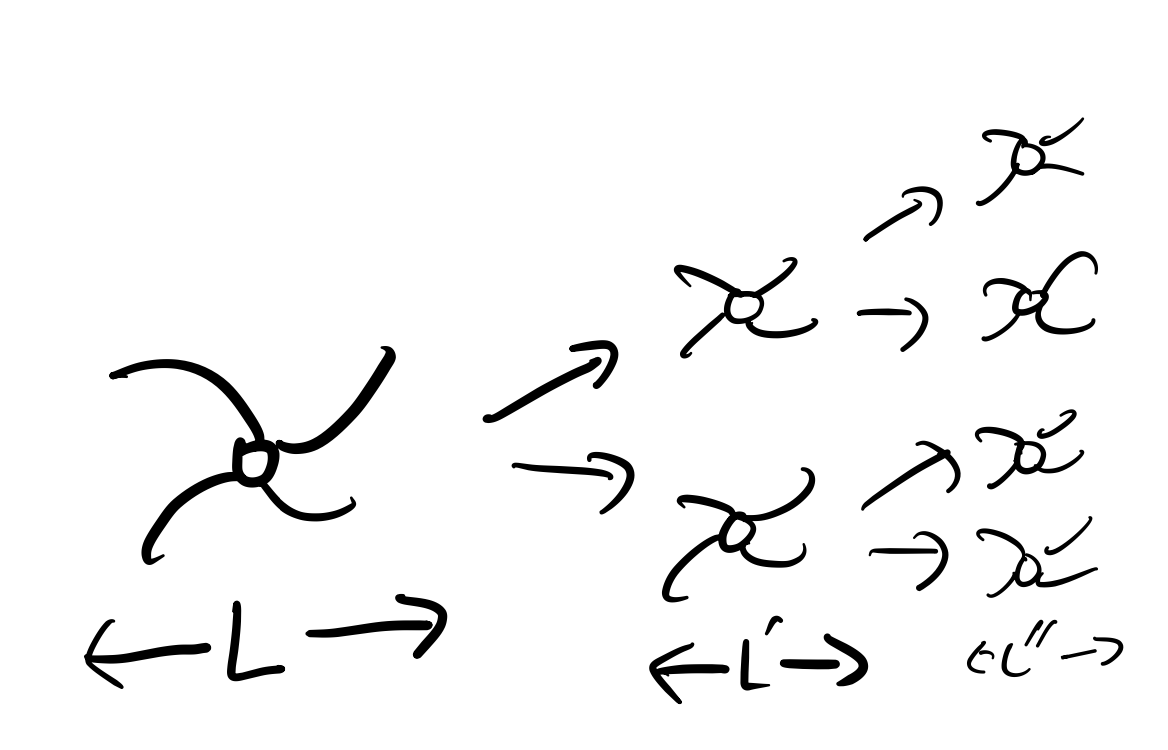
\includegraphics[scale=0.35]{Lectures/Images/lec11-splittingeddy.png}
\end{center}

We can also consider the time scale:
\begin{equation}
    \tau_l \sim \frac{l}{v_l}
\end{equation}
where $l$ is the eddy size and $v_l$ the characteristic velocity. This we call the ``eddy turnover time''. Let's now think about the energy flux that occurs between each scale, e.g. $l \to l/2$. The process that mediates this flux of energy is that the eddy splits. This flux will be equal to the kinetic energy divided by the turnover time:
\begin{equation}
    \Pi_l \sim \frac{v_l^2}{\tau_l} \sim \frac{v_l^3}{l}
\end{equation}
The assumption of Kolmogorov was that this $\Pi_l$ was a constant, until we go to a dissipative scale:
\begin{equation}
    \Pi_l \sim \frac{v_l^3}{l} = \e
\end{equation}
From which:
\begin{equation}
    v_l \sim (\e l)^{1/3}
\end{equation}
\begin{equation}
    \tau_l \sim \e^{-1/3}l^{2/3} \sim \e^{-1/3}k^{-2/3}
\end{equation}
where we have used $\frac{1}{l} \sim k$. The energy per unit mass per eddy is:
\begin{equation}
    \text{KE} \sim \frac{1}{2}v_l^2 \sim E(k)dk
\end{equation}
Hence:
\begin{equation}
    E(k)l^{-1} \sim \left[(\e l)^{1/3}\right]^2 \implies E(k) \sim e^{2/3}l^{5/3} \sim \e^{2/3}k^{-5/3}
\end{equation}
so we reproduce the power-law dependence on $k$ that we expect!

Next time, either we continue with turbulence, but with a caveat - we put the odd viscosity term in, and see what happens to the spectrum. Or, we look at how turbulence changes the analysis of fluid flow around the sphere.
\section{Stokes' Flow with Odd Viscosity}

\emph{(Guest lecture by Tali Khain)}

Today, we'll discuss the Stokes' fluid flow problem around a sphere, first reviewing the problem for a normal fluid, then studying what happens when we add odd viscosity.

\subsection{The Stokeslet}
We consider the Reynold's number:
\begin{equation}
    \text{Re} = \frac{\rho U L}{\mu}
\end{equation}
which is low, e.g., when we look at small particles travelling in a fluid (as $L$ in this case is small). In this scenario, the Navier-Stokes equation reduces to:
\begin{equation}
    -\nabla p + \mu \nabla^2 \v{v} = -\v{F}(\v{r})
\end{equation}
and we also assume that the fluid is incompressible:
\begin{equation}
    \nabla \cdot \v{v} = 0
\end{equation}
Since these equations are linear in $p, \v{v}$, analytical progress is possible. 

We can make an analogy with electrostatics, where we have the Poisson equation:
\begin{equation}
    \nabla^2 \phi = 4\pi \rho(\v{r})
\end{equation}
The first problem we solve is that for a point charge, where we have the Green's function solution:
\begin{equation}
    \nabla^2 G = q\delta^3(\v{r})
\end{equation}
which is the first order/monopole term in the multiple expansion when looking for the potential $\phi(\v{r})$ of an arbitrary charge distribution $\rho(\v{r})$.

The analogy we make is charge $\leftrightarrow$ forces, potential $\leftrightarrow $ velocity. Today, we compute the Green's function of the Stoke's equations, which tells us the response of a fluid to a point force.

\begin{center}
    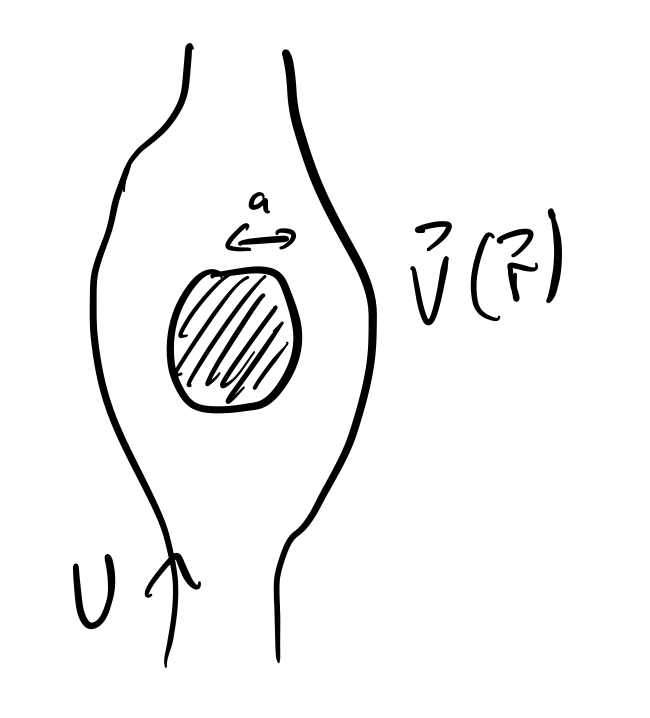
\includegraphics[scale=0.35]{Lectures/Images/lec12-sphereinfluid.png}
\end{center}

A common problem we study in fluid mechanics is we study a spherical particle in a medium, under force $\v{F}$ and fluid velocity field $\v{v}$. We work in the overdamped regime, where $F \sim U$. The stokes drag is then given as:
\begin{equation}
    U \sim \frac{F}{6\pi \mu a}
\end{equation}
with $a$ the length scale of the sphere. The velocity field is given by:
\begin{equation}
    \v{v} = \frac{\v{F}}{8\pi\mu}\cdot (1 + \frac{a^2}{6}\nabla^2)\mathbb{G}
\end{equation}
in the regime of small $a$ we can neglect the $\nabla^2$ term, so:
\begin{equation}
    \v{v} = \frac{\v{F}}{8\pi\mu}\cdot \mathbb{G}
\end{equation}
we can interpret this as like solving for the ``monopole'' term/far field limit in electrostatics. This primary Green's function is what is known as the Stokeslet.

\subsection{Solving Navier-Stokes with Point Flow Source}
We solve the equations:
\begin{equation}
    -\nabla p + \mu \nabla^2 \v{v} = -\v{F}\delta^3(\v{r})
\end{equation}
\begin{equation}
    \nabla \cdot \v{v} = 0
\end{equation}
by going into fourier space; we have the Fourier and inverse Fourier transforms:
\begin{equation}
    f(\v{k}) = \int d^3\v{r}f(\v{r})e^{-i\v{k}\cdot\v{r}}
\end{equation}
\begin{equation}
    f(\v{r}) = \frac{1}{(2\pi)^3}\int d^3\v{k}f(\v{k})e^{i\v{k} \cdot \v{r}}
\end{equation}
so then $\nabla \to i\v{k}$ in Fourier space. In $\v{k}$-space the equations become:
\begin{equation}
    -i\v{k}p - \mu k^2\v{v} = -\v{F}
\end{equation}
\begin{equation}
    \v{k} \cdot \v{v} = 0
\end{equation}
to eliminate the velocity term, we apply $\v{k} \cdot$ to the first equation, which yields:
\begin{equation}
    -ik^2p - \mu k^2 \v{k} \cdot \v{v} = -\v{k} \cdot \v{F} \implies -k^2p = -\v{k} \cdot \v{F} \implies p = -i\frac{\v{k}\cdot\v{F}}{k^2}
\end{equation}
Plugging back in this expression for the pressure to solve for the velocity:
\begin{equation}
    -i\v{k}\left(-i\frac{\v{k}\cdot\v{F}}{k^2}\right) - \mu k^2\v{v} = -\v{F} \implies \v{v} = \frac{1}{\mu k^2}\left[\v{F} - \v{k}\left(\frac{\v{k} \cdot \v{F}}{k^2}\right)\right] = \frac{1}{\mu k^2}\left[\II - \frac{\v{k} \v{k}}{k^2}\right]\cdot \v{F}
\end{equation}
where $\v{k}\v{k}$ is the matrix $(\v{k}\v{k})_{ij} = k_ik_j$. Our Green's function in Fourier space is therefore:
\begin{equation}
    \mathbb{G}(\v{k}) = \frac{1}{\mu k^2}\left[\II - \frac{\v{k} \v{k}}{k^2}\right]
\end{equation}
And our velocity field in position space is obtained by taking the inverse Fourier transform:
\begin{equation}\label{eq:intermediatev}
    \v{v}(\v{r}) = \frac{1}{(2\pi)^3}\int d^3\v{k}\frac{1}{\mu k^2}\left[\II - \frac{\v{k}\v{k}}{k^2}\right]\cdot\v{F}e^{i\v{k} \cdot \v{r}}
\end{equation}
This is the tricky part - going back to real space. Formally, we solve these by contour integration in the complex plane. But, for this class we will take a few shortcuts and use results that you may know already. From electrostatics, recall:
\begin{equation}
    \nabla^2 \phi = -\delta^3(\v{r})
\end{equation}
\begin{equation}
    \phi(\v{r}) = \frac{1}{4\pi r} = \frac{1}{(2\pi)^3}\int d^3\v{k} \frac{1}{k^2}e^{i\v{k} \cdot \v{r}}
\end{equation}
from which:
\begin{equation}
    -k^2\phi = -1 \implies \phi = \frac{1}{k^2}
\end{equation}
This gives us the first term. The analogous process for the biharmonic equation is:
\begin{equation}
    \nabla^4 \psi(\v{r}) = -\delta^3(\v{r})
\end{equation}
so:
\begin{equation}
    \psi(\v{r}) = \frac{r}{8\pi}
\end{equation}
so then:
\begin{equation}
    k^4\psi = -1 \implies \psi = -\frac{1}{k^4}
\end{equation}
and so we have the equation:
\begin{equation}
    \psi(\v{r}) = \frac{r}{8\pi} = -\frac{1}{(2\pi)^3}\int d^3k \frac{1}{k^4}e^{i\v{k} \cdot \v{r}}
\end{equation}
but we notice that we don't just require the inverse fourier transform of $\frac{e^{i\v{k} \cdot \v{r}}}{k^4}$ but with the $\v{k}\v{k}$ in the numerator, so we take two derivatives:
\begin{equation}
    \nabla \nabla(\frac{r}{8\pi}) = -\frac{1}{(2\pi)^3}\int d^3k\frac{\v{k}\v{k}}{k^4}e^{i\v{k} \cdot \v{r}}
\end{equation}
But what exactly is the object on the LHS? Well:
\begin{equation}
    \p_i \p_j\left(\frac{r}{8\pi}\right) = \frac{1}{8\pi}\p_i\left(\frac{r_i}{r}\right) = \frac{1}{8\pi}\left[\frac{\delta_{ij}r - \frac{r_i}{r}r_j}{r^2}\right] = \frac{1}{8\pi}\left[\frac{\delta_{ij}}{r} - \frac{r_ir_j}{r^3}\right] = \frac{1}{8\pi}\left[\frac{\II}{r} - \frac{\v{r}\v{r}}{r^3}\right]
\end{equation}

So combining these two results, we can return back to our velocity field integral in Eq. \eqref{eq:intermediatev} to obtain:
\begin{equation}
    \v{v}(\v{r}) = \frac{1}{\mu}\left[\frac{\II}{4\pi r} - \frac{\II}{8\pi r} + \frac{\v{r} \v{r}}{8\pi r^3}\right]\cdot\v{F} = \frac{1}{8\pi \mu r}\left[\II + \frac{\v{r}\v{r}}{r^2}\right]\cdot\v{F}
\end{equation}
we have thus obtained the Green's function in real space:
\begin{equation}
    \mathbb{G}(\v{r}) = \frac{1}{8\pi \mu 4}\left[\II + \frac{\v{r}\v{r}}{r^2}\right]
\end{equation}
and we can also proceed to solve for the pressure $p(\v{r})
$. This is what happens for a normal fluid - what happens when we add odd viscosity?

\subsection{Solving Navier-Stokes with Odd Viscosity}
If we now also have odd viscosity, the first equation of Navier-Stokes is modified to be:
\begin{equation}
    -\nabla p + \m{\mu & \eta^0 & 0 \\ -\eta^0 & \mu & 0 \\ 0 & 0 & \mu}\nabla^2\v{v} = -\v{F}\delta^3(\v{r})
\end{equation}
with the $\eta^0$ term corresponding to the odd viscosity coefficient. We have chosen the rotation axis of the fluid molecules (which gives rise to the odd viscosity) to be $\hat{\v{z}}$ and hence this is why the odd viscosity terms only appear in $xy$, and the above matrix is not isotropic. Defining $\gamma = \frac{\eta^0}{\mu}$, the above equation becomes:
\begin{equation}
    -\nabla p + \mu\m{1 & \gamma & 0 \\ -\gamma & 1 & 0 \\ 0 & 0 & 1}\nabla^2\v{v} = -\nabla p + \mu\mathbb{M}\nabla^2 \v{v} = -\v{F}\delta^3(\v{r})
\end{equation}
Again going into Fourier space:
\begin{equation}\label{eq:fourierodd}
    -i\v{k}p - \mu \mathbb{M}k^2\v{v} = -\v{F}
\end{equation}
\begin{equation}
    \v{k} \cdot \v{v} = 0
\end{equation}
Let us multiply the first equation by $\mathbb{M}^{-1}$:
\begin{equation}
    -i\mathbb{M}^{-1}\v{k}p - \mu k^2 \v{v} = -\mathbb{M}^{-1}\v{F}
\end{equation}
and now multiplying this by $\v{k}\cdot$ to get rid of the velocity term:
\begin{equation}
    -i\v{k} \cdot \mathbb{M}^{-1}\v{k}p = -\v{k}\cdot \mathbb{M}^{-1}\v{F}
\end{equation}
Solving for $p$:
\begin{equation}
    p = -i\frac{\v{k} \cdot \mathbb{M}^{-1}\v{F}}{\v{k} \cdot \mathbb{M}^{-1}\v{k}}
\end{equation}
We can now plug this back into Eq. \eqref{eq:fourierodd} to solve for the velocity:
\begin{equation}
    -\v{k}\frac{\v{k} \cdot \mathbb{M}^{-1}\v{F}}{\v{k} \cdot \mathbb{M}^{-1}\v{k}} - \mu \mathbb{M}k^2\v{v} = -\v{F}
\end{equation}
\begin{equation}
    \v{v} = \frac{1}{\mu k^2}\mathbb{M}^{-1}\left[\v{F} - \v{k}\left(\frac{\v{k} \cdot \mathbb{M}^{-1}\v{F}}{\v{k} \cdot \mathbb{M}^{-1}\v{k}}\right)\right] = \frac{\mathbb{M}^{-1}}{\mu k^2}\left[\II - \frac{\v{k}(\v{k}\cdot \mathbb{M}^{-1})}{\v{k}\cdot(\mathbb{M}^{-1}\v{k})}\right]\cdot\v{F}
\end{equation}
Now, considering the limit $\gamma = \frac{\eta_0}{\mu} \ll 1$, we can write:
\begin{equation}
    \mathbb{M} = \II + \gamma \e
\end{equation}
with:
\begin{equation}
    \e = \m{0 & 1 & 0 \\ -1 & 0 & 0 \\ 0 & 0 & 0}
\end{equation}
where then:
\begin{equation}
    \mathbb{M}^{-1} = \II - \gamma \e
\end{equation}
Then in this small $\gamma$ limit:
\begin{equation}
    \v{k} \cdot \mathbb{M}^{-1}\v{k} = k^2 - \gamma \v{k} \cdot \e \v{k} = k^2
\end{equation}
where the last term vanishes as:
\begin{equation}
    \v{k} \cdot \e \v{k} = \m{k_x & k_y & k_z}\m{k_y \\ -k_x \\ 0} = k_xk_y - k_yk_x = 0
\end{equation}
So the velocity becomes:
\begin{equation}
    \v{v} = \frac{\II - \gamma \e}{\mu k^2}\left[\II - \frac{\v{k}\v{k}}{k^2} + \frac{\gamma \v{k}\v{k}\e}{k^2}\right]\cdot\v{F} = \frac{1}{\mu k^2}\left[\II - \frac{\v{k}\v{k}}{k^2} + \frac{\gamma\v{k}\v{k}\e}{k^2} - \gamma \e + \frac{\gamma \e\v{k}\v{k}}{k^2} + \mathcal{O}(\gamma^2)\right]\cdot\v{F}
\end{equation}
The nice part of the expression is that the terms appearing just look like $\frac{\v{k}\v{k}}{k^2}$ multiplied by $\e$s. We define some helper matrices:
\begin{equation}
    \mathbb{G}^1 = \frac{\II}{\mu k^2}, \mathbb{G}^2 = \frac{\v{k}\v{k}}{\mu k^4}
\end{equation}
which allows us to write the velocity as:
\begin{equation}
    \v{v} = [\mathbb{G}^1 - \mathbb{G}^2 + \gamma \mathbb{G}^2\e - \gamma\e \mathbb{G}^1 + \gamma \e \mathbb{G}^2]\cdot \v{F}
\end{equation}
Just to clear up the notation, when we write $\v{v} \sim \gamma \v{k}\v{k}\e\v{F}$ we mean:
\begin{equation}
    v_i \sim k_ik_j\e_{jk}F_k
\end{equation}
and for $\v{v} \sim \e\v{k}\v{k} \cdot \v{F}$ we mean:
\begin{equation}
    v_i \sim \e_{ij}k_jk_kF_k
\end{equation}
Denoting:
\begin{equation}
    v_\gamma = \gamma \mathbb{G}^2 \e - \gamma \e \mathbb{G}^1 + \gamma \e \mathbb{G}^2
\end{equation}
in real space this looks like:
\begin{equation}
    v_\gamma(\v{r}) = \frac{\gamma}{8\pi\mu}\left[\frac{\e}{r} - \frac{\v{r}\v{r}\e}{r^3} - \frac{2\e}{r} + \frac{\e}{r} - \frac{\e\v{r}\v{r}}{r^3}\right]\cdot\v{F} = -\frac{\gamma}{8\pi\mu}\left[\frac{\v{r}\v{r}\e}{r^3} + \frac{\e\v{r}\v{r}}{r^3}\right]\cdot\v{F}
\end{equation}
so we have our Green's function (to first order in the odd viscosity):
\begin{equation}
    \mathbb{G}_\gamma(\v{r}) = -\frac{\gamma}{8\pi\mu}\left[\frac{\v{r}\v{r}\e}{r^3} + \frac{\e\v{r}\v{r}}{r^3}\right]
\end{equation}
the decay of the velocity field goes as $\sim \frac{1}{r}$ both in the normal and odd fluid cases, but the form of these matrices are different. Let us write out the full Green's function:
\begin{equation}
    \begin{split}
        \mathbb{G}_{\text{full}}(\v{r}) &= \mathbb{G}(\v{r}) + \mathbb{G}_\gamma(\v{r}) 
        \\ &= \frac{1}{8\pi \mu r^3}\m{2x^2 + y^2 + z^2 & xy & xz \\ xy & x^2 + 2y^2 + z^2 & yz & yz \\ xz & yz & x^2 + y^2 + 2z^2} - \frac{\gamma}{8\pi\mu r^3}\m{0 & x^2 + y^2 & yz \\ -(x^2 + y^2) & 0 & -xz \\ -yz & xz & 0}
    \end{split}
\end{equation}

\subsection{Velocity Field from Stokeslet}

\begin{center}
    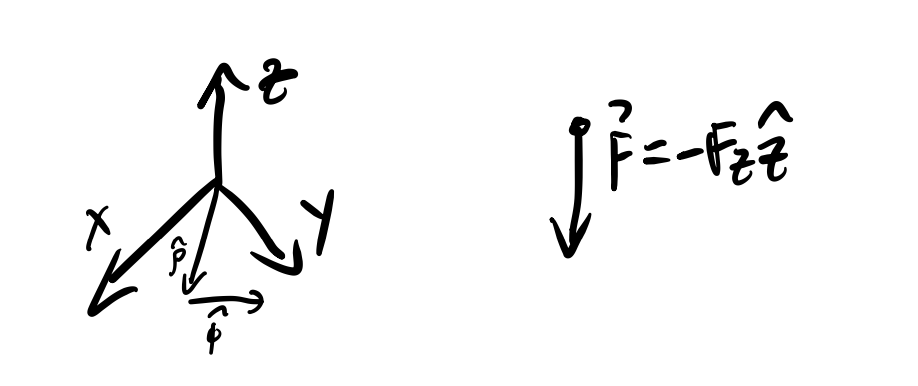
\includegraphics[scale=0.35]{Lectures/Images/lec12-coordinates.png}
\end{center}

What would a velocity field look like? Supposing $\v{F} = -F_z\zhat$, for the normal Stokeslet we have:
\begin{equation}
    \v{v}_0(\v{r}) = -\frac{F_z}{8\pi\mu r^3}\m{xz \\ yz \\ x^2 + y^2 + 2z^2}
\end{equation}
Looking at the magnitude of the velocity in the $xy$-plane (radial), we have:
\begin{equation}
    v^\rho_0(\v{r}) = \frac{xv_x + yv_y}{\sqrt{x^2 + y^2}} = -\frac{F_z}{8\pi \mu r^3}z\left(\frac{x^2 + y^2}{\sqrt{x^2 + y^2}}\right) = -\frac{F_z}{8\pi \mu r^3}z\rho
\end{equation}
and looking at the magnitude of the velocity in $\phi$ (tangential) we have:
\begin{equation}
    v^\phi_0(\v{r}) = \frac{-yv_x + xv_y}{\sqrt{x^2 + y^2}} = 0
\end{equation}

What about for the velocity arising from the odd viscosity? We find:
\begin{equation}
    \v{v}_\gamma(\v{r}) = \frac{\gamma}{8\pi \mu r^3}\m{yz \\ -xz \\ 0}
\end{equation}
where we find:
\begin{equation}
    v^\rho_\gamma(\v{r}) = 0
\end{equation}
\begin{equation}
    v^\phi_\gamma(\v{r}) = -\frac{\gamma F_z}{8\pi \mu r^3}\rho z
\end{equation}
So the leading order corrections to the velocity field due to odd viscosity are to induce some rotational/tangential flow!

\begin{center}
    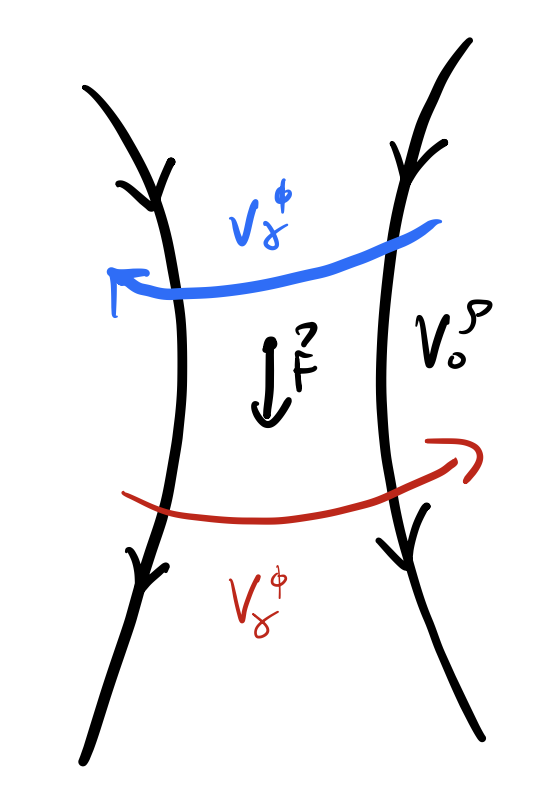
\includegraphics[scale=0.35]{Lectures/Images/lec12-velocityfield.png}
\end{center}

Note that we did the calculation perturbatively, but we are able to do the calculation for any $\gamma$. The flows in 3D look like:

\begin{center}
    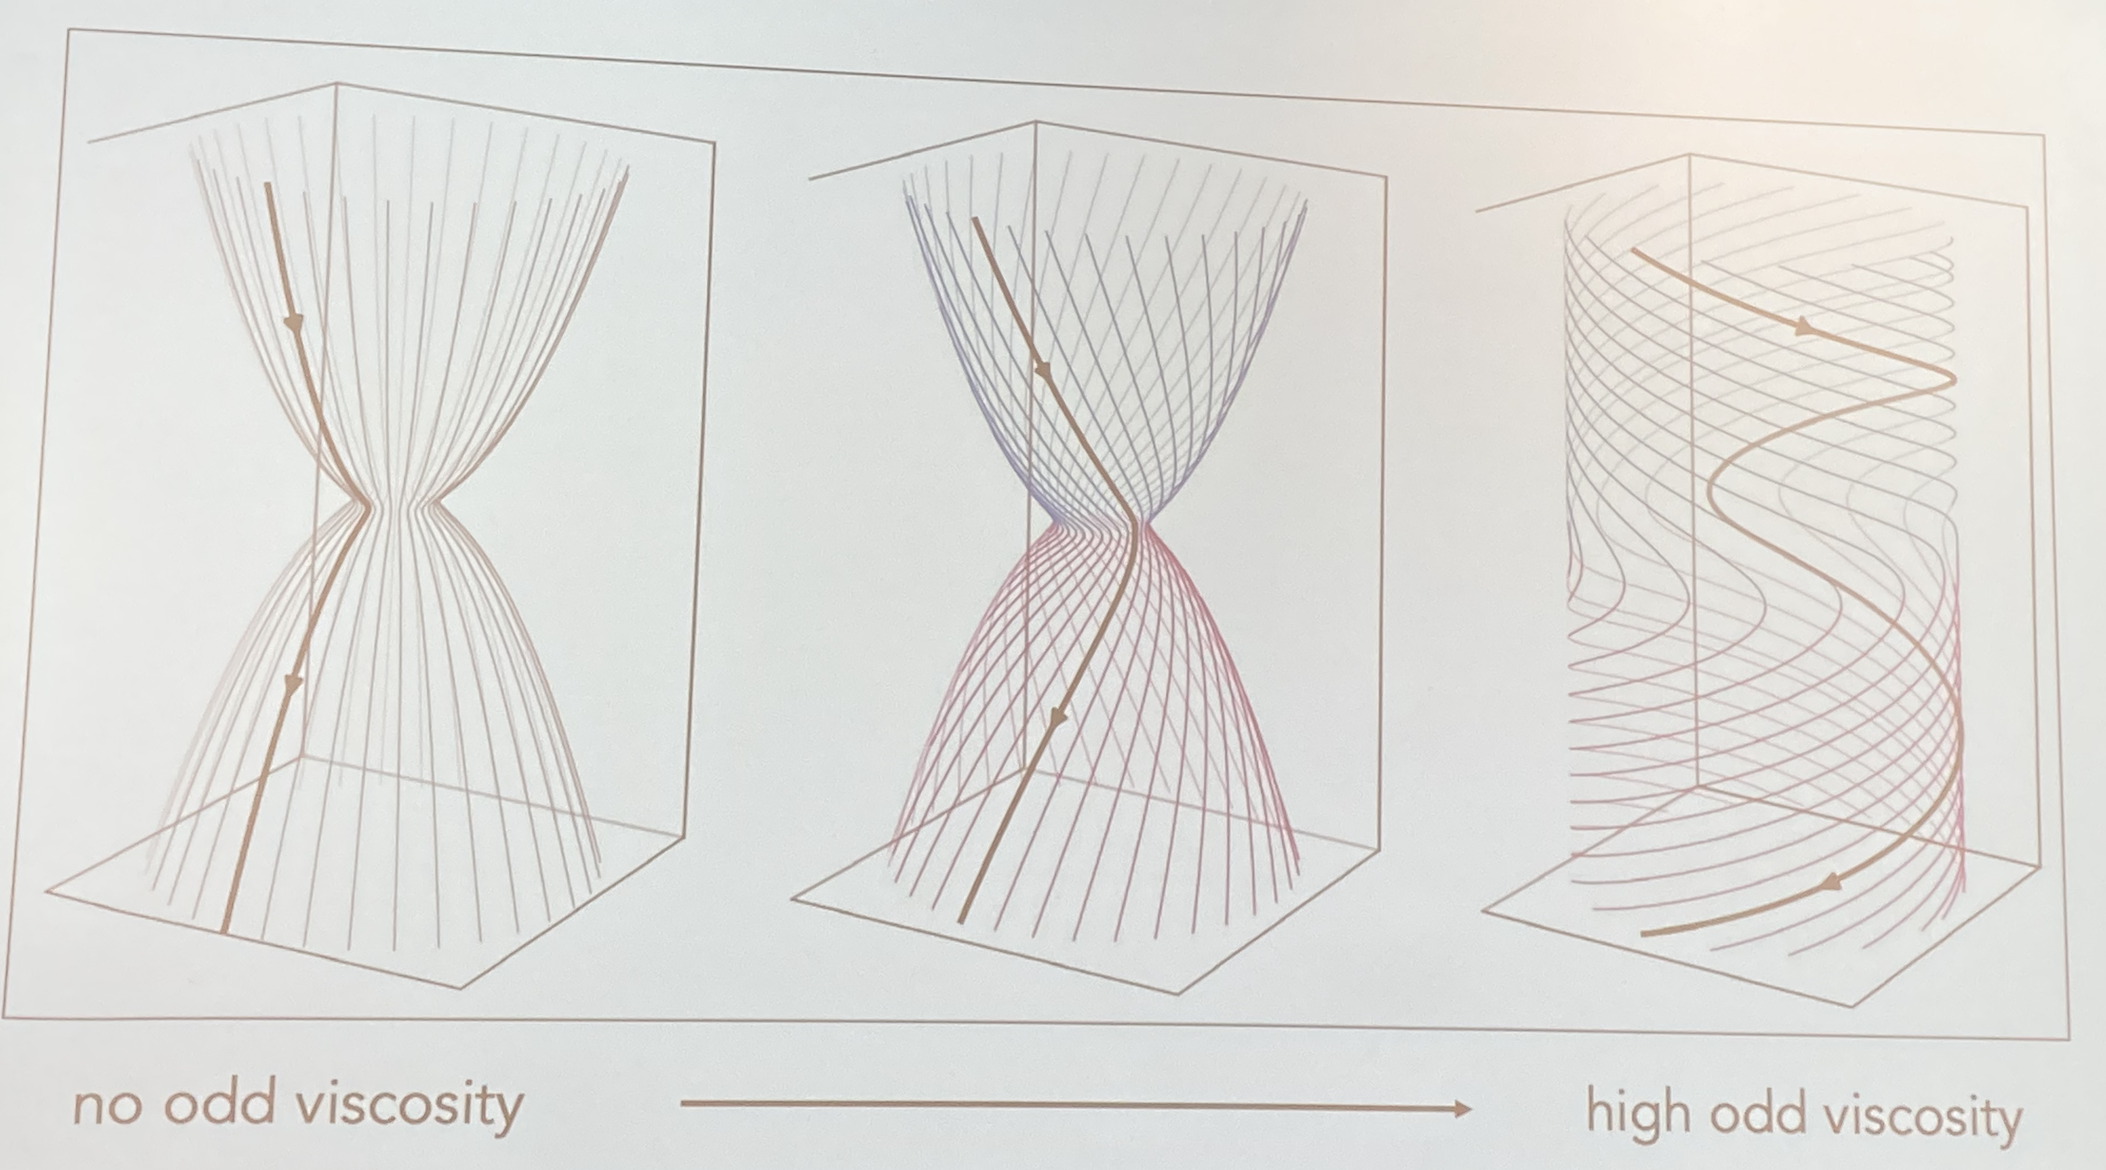
\includegraphics[scale=0.35]{Lectures/Images/lec12-velocityfieldstokeslet.png}
\end{center}

\subsection{Velocity Field with Sphere}
If we are interested in how the fluid moves past the sphere, we now have the correction (for the normal fluid case):
\begin{equation}
    \v{v} = \frac{\v{F}}{8\pi \mu}[1 + \frac{a^2}{6}\nabla^2]\mathbb{G}
\end{equation}
as in close to the sphere we are not able to neglect the $a^2$ term/treat it as small. The first order correction comes in the form of an azimuthal flow:
\begin{equation}
    v_\phi(r, z) = \frac{3aVrz(r^2 + z^2 - a^2)}{4(r^2 + z^2)^{5/2}}
\end{equation}

\begin{center}
    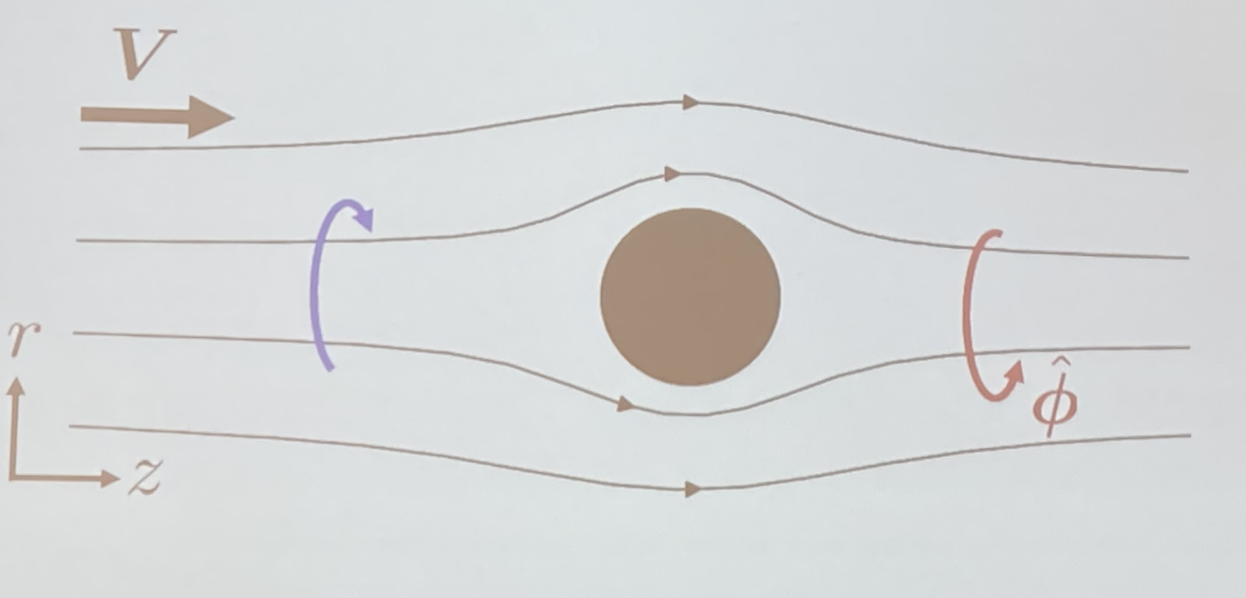
\includegraphics[scale=0.35]{Lectures/Images/lec12-oddsphere.png}
    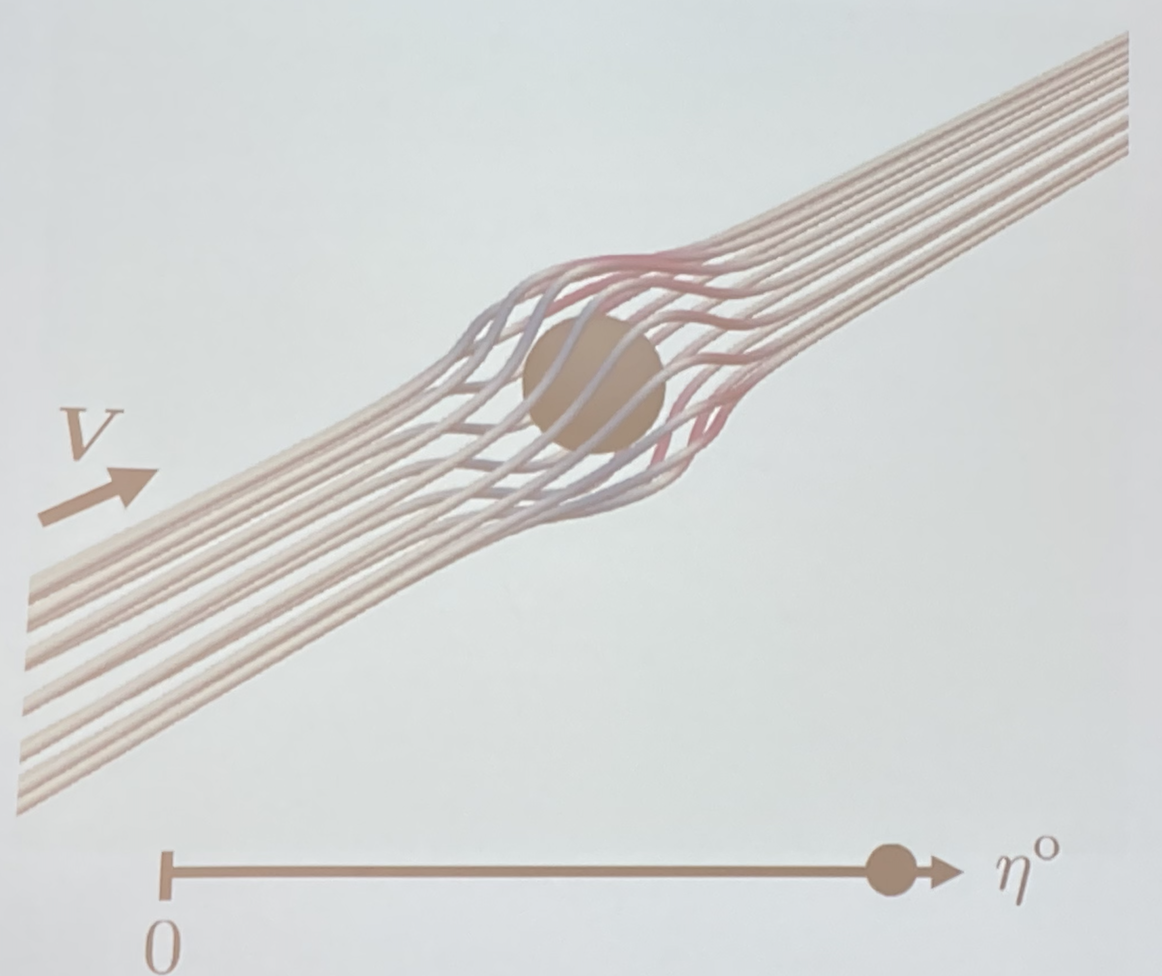
\includegraphics[scale=0.35]{Lectures/Images/lec12-oddsphere3d.png}
\end{center}

Also - odd viscosity in fluid causes velocity of sphere in a tilted direction (a ``lift force'') when an external force is applied; this is due to the asymmetric mobility matrix:
\begin{equation}
    \m{V_x \\ V_y \\ V_z} = \frac{1}{6\pi\mu a}\m{1 & \e/2 & 0 \\ -\e/2 & 1 & 0 \\ 0 & 0 & 1}\m{F_x \\ F_y \\ F_z}
\end{equation}

\begin{center}
    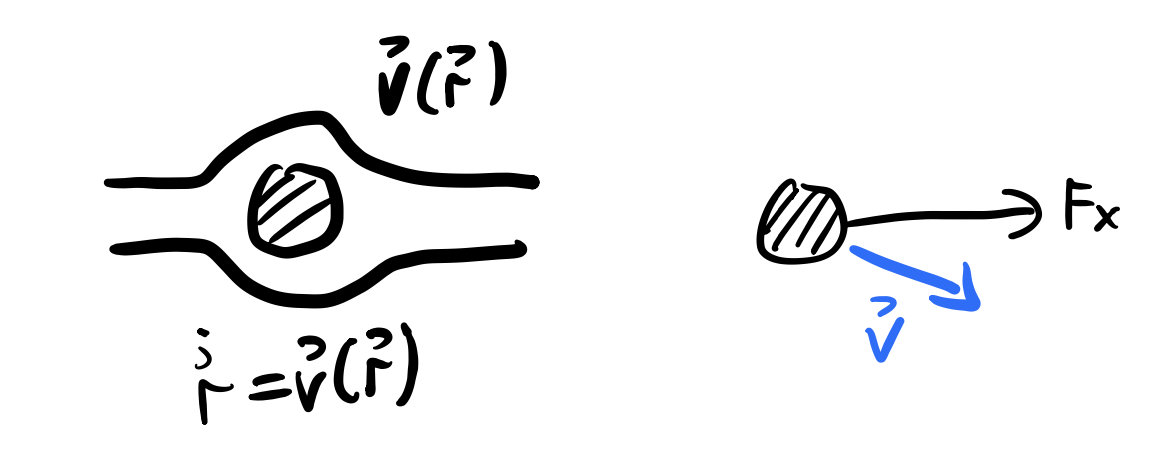
\includegraphics[scale=0.35]{Lectures/Images/lec12-liftforce.png}
\end{center}

Can also look at the many-body version of this problem (``many-body sedimentation''), wherein a cloud of such particles interact through the fluid. The particles in the cloud can display radial/tangential motion, and the competition between these two can change the shape of the cloud of particles (from toroidal to elliptical).
\section{Turbulence II}

Last time we saw some exact results for Stokes' flow (fluid flow at low Reynolds number) in the presence of odd viscosity. Usually, at higher Reynolds number, the calculations become less and less analytically tractable. But there are some aspects that become accessible to study via a statistical mechanics lens - we discuss them today.

\subsection{Review}
We looked at $\log E(k)$, the logartihm of the power spectrum:

\begin{center}
    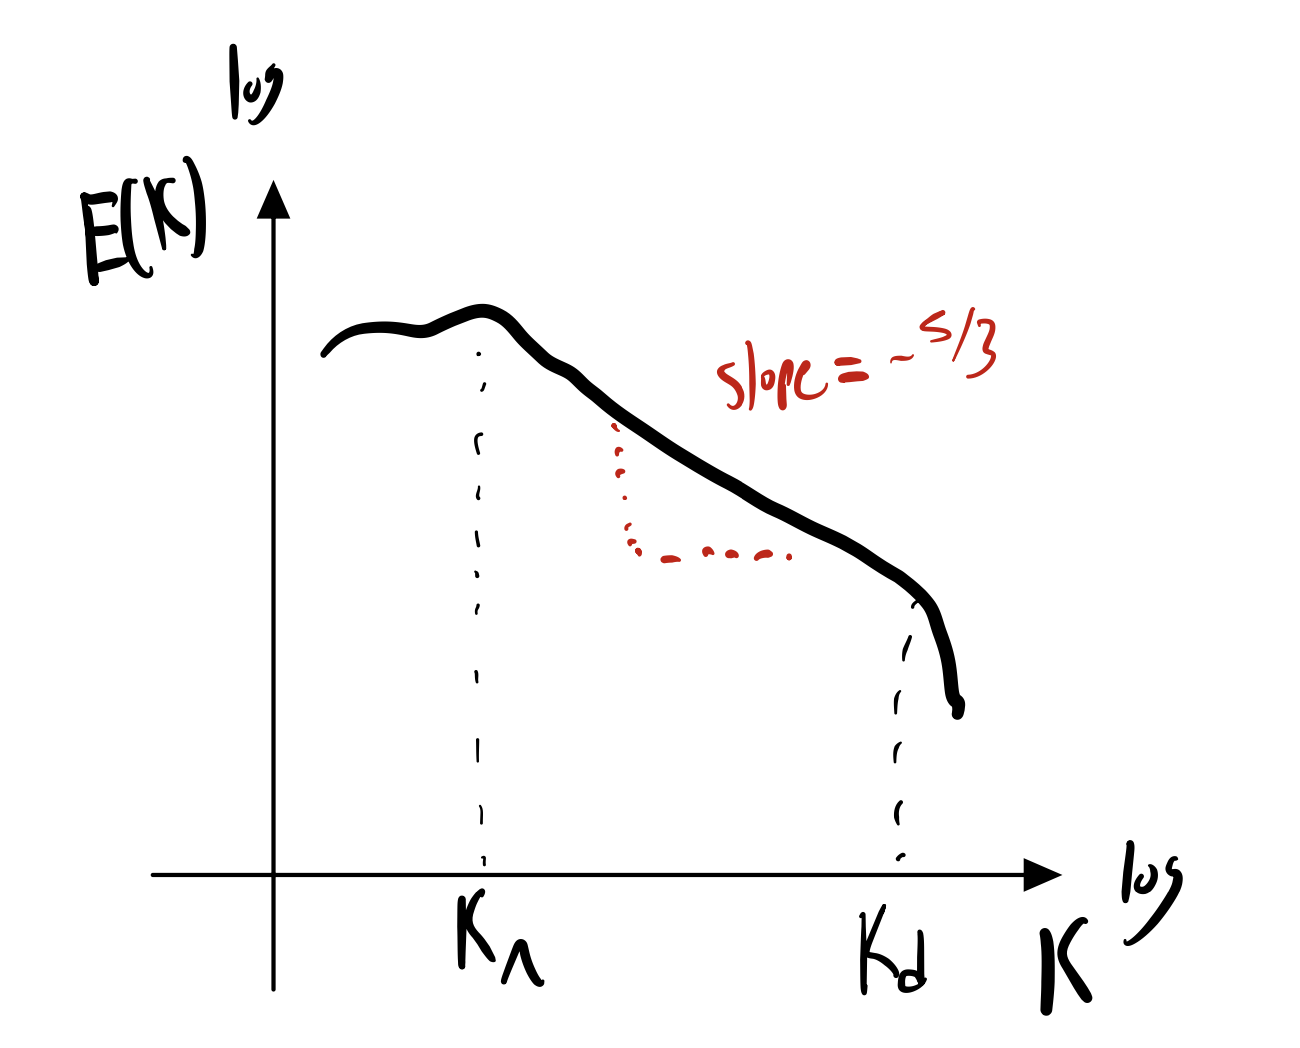
\includegraphics[scale=0.35]{Lectures/Images/lec11-spectrum.png}
\end{center}
where in the inertial range $k_\lambda \leq k \leq k_d$ (where the dissipative scale $k_d$ is set by when $\text{Re} = \frac{UL}{\nu} \sim 1$). Here, we have:
\begin{equation}
    E(k) \sim \e^{2/3}k^{-5/3}
\end{equation}
and the Navier-Stokes equations reduce to:
\begin{equation}
    \text{Re}(\p_t \v{v} + \v{v} \cdot \nabla \v{v}) = \nabla p + v \nabla^2\v{v}
\end{equation}
Where a key assumption in the derivation was that the energy flux was constant:
\begin{equation}
    \Pi_l \sim \frac{v_l^2}{\tau_l} \sim \frac{v_l^3}{l} = \text{const.} = \e
\end{equation}

\subsection{Estimating the dissipative scale}
Recall back to a particle falling in a viscous medium - the power dissipated is given by $P = \v{F} \cdot \v{v} \propto \eta v(v) = \eta v^2$. In continuum theory, we promote this to:
\begin{equation}
    P \propto \eta_{ijkl}v_{ij}v_{kl}
\end{equation}
with $v_{ij} = \p_i v_j$. 

So, let us estimate:
\begin{equation}
    P \sim \nu(\p_i v_j)^2
\end{equation}
The first scale at which dissipation starts to become non-negligible is at $k = k_d$. So, estimating the power at this point:
\begin{equation}
    P \sim \nu \left(\frac{v_d}{\eta_d}\right)^2
\end{equation}
with $\eta_d \sim \frac{1}{k_d}$ - this ensures that:
\begin{equation}
    \text{Re} \sim \frac{v_d\eta_d}{\nu} \sim 1.
\end{equation}
Physically, we can imagine that $v_d$ is the smallest scale speed and $\eta_d$ is the length corresponding to the smallest eddy size. Now, we make the assumption that all of the energy injected into the system at $k = k_\Lambda$ is dissipated at $k = k_d$. So, our estimate of the energy flux is:
\begin{equation}
    \e \sim \nu \left(\frac{v_d}{\eta_d}\right)^2
\end{equation}
Now, we can say that, since the effective Reynolds is $\text{Re} \sim 1$ at $k_d$:
\begin{equation}
    v_d \sim \frac{\nu}{\eta_d}
\end{equation}
Now, we can say:
\begin{equation}
    \eta \sim \nu \left(\frac{\frac{\nu}{\eta_d}}{\eta_d}\right)^2 = \frac{\nu^3}{\eta_d^4}
\end{equation}
Thus isolating for $\eta_d$ and thus $k_d$:
\begin{equation}
    \eta_d \sim \left(\frac{\nu^3}{\e}\right)^{1/4} \implies k_d \sim \left(\frac{\e}{\nu^3}\right)^{1/4}
\end{equation}
Now, let us write $\e = \frac{U^3}{L}$ (where $U$ is the macroscopic speed scale in which we inject energy), so:
\begin{equation}
    \eta_d \sim \left(L\frac{\nu^3}{U^3}\right)^{1/4}
\end{equation}
Now, by multiplying this by one, we can write this in terms of the original Reynolds number $\text{Re} = \frac{UL}{\nu}$:
\begin{equation}
    \eta_d \sim \left(\frac{\nu^3}{U^3L^3}L^4\right)^{1/4} \sim \text{Re}^{-3/4}L
\end{equation}
hence we have the conclusion:
\begin{equation}
   \boxed{\frac{\eta_d}{L} \sim \frac{1}{\text{Re}^{3/4}}}
\end{equation}
where $\text{Re}$ is the Reynolds number at injection.

Let's now plug in the Reynolds number for a given experimental setup. We consider an experimental setup where we have fluid of Reynolds number $\text{Re} \sim 10^3$ flowing through a grid of grid size $l \sim \text{1}\si{cm}$:

\begin{center}
    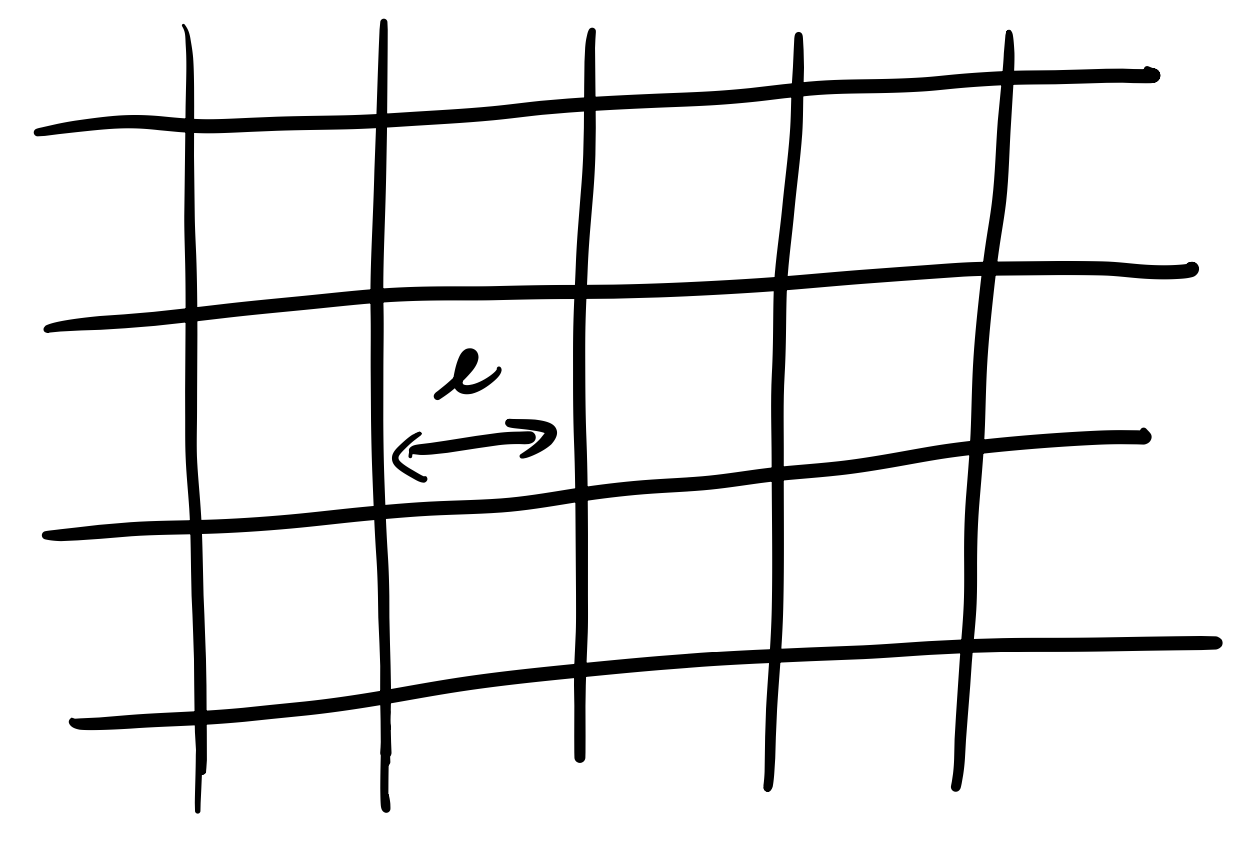
\includegraphics[scale=0.35]{Lectures/Images/lec13-lattice.png}
\end{center}

Which yields:
\begin{equation}
    \eta_d \sim 0.06\si{mm}
\end{equation}
We can see from this simple calculation how this scaling is quite unfavourable for experimentalists - we have sublinear scaling in the Reynolds number. To span many decades is quite difficult.

\subsection{Enstrophy and the Zeroth Law of Turbulence}
We wish to evaluate the power/rate at which we lose energy due to viscosity, $\pd{E}{t}$. We start with the change in kinetic energy of the system, and rewrite it using Navier-Stokes:
\begin{equation}
    \frac{1}{2}\rho_0\frac{\partial(\v{u}^2)}{\partial t} = \rho_0 \v{u}\cdot \dpd{\v{u}}{t} = \rho_0 \v{u}\cdot\left(-\v{u}\cdot\nabla\v{u} - \frac{\nabla p}{\rho_0} + \nu\nabla^2\v{u}\right)
\end{equation}
Now, we rewrite:
\begin{equation}
    \v{u} \cdot \nabla^2 \v{u} = -\v{u} \cdot (\nabla \times (\nabla \times \v{u})) = -\v{u} \cdot (\nabla \times \gv{\omega})
\end{equation}
where we define $\gv{\omega} = \nabla \times \v{u}$ the vorticity, and in the above vector field identity we have assumed incompressibility $\nabla \cdot \v{u} = 0$. We can further rewrite:
\begin{equation}
    \v{u} \cdot \nabla^2\v{u} = \nabla\cdot(\v{u} \times \gv{\omega}) - \gv{\omega}^2
\end{equation}
Our expression for the kinetic energy loss becomes (again using $\nabla \cdot \v{u} = 0$ where necessary):
\begin{equation}
    \frac{1}{2}\rho_0\frac{\partial(\v{u}^2)}{\partial t} = -\rho_0 \v{u} \cdot \nabla\left(\frac{u^2}{2}\right) - \nabla \cdot (p\v{u} - \rho_0 \nu(\v{u} \times \gv{\omega})) - \rho_0 \nu\gv{\omega}^2
\end{equation}
Hence:
\begin{equation}
    \pd{E}{t} = -\nabla\cdot\underbrace{\left[\left(\rho_0\frac{\v{v}^2}{2} + p\right)\v{u} - \rho_0\nu \v{u} \times \gv{\omega}\right]}_{\text{flux}} - \underbrace{\rho_0 \nu \gv{\omega}^2}_{\text{source/sink}}
\end{equation}
If we assume that $\v{u} = \v{0}$ sufficiently quickly at the boundaries of the system, or we have periodic boundary conditions, we may drop the flux term, and we thus only study:
\begin{equation}
    \boxed{\dpd{E}{t} = -\rho_0 \nu\gv{\omega}^2}
\end{equation}
so the energy loss is proportional to the vorticity squared.

The volume version of this is:
\begin{equation}
    \dpd{}{t}\iiint E dV = -\oiint \v{F} \cdot \hat{\v{n}}dS - \rho_0v \iiint \gv{\omega}^2 dV
\end{equation}

In $d$-dimensions, we can define the enstropy per unit volume (area) as:
\begin{equation}
    \Omega = \frac{\text{Enstrophy}}{L^d} = \frac{1}{2}\avg{\gv{\omega}^2}
\end{equation}
Wherein:
\begin{equation}
    \dpd{\avg{E}}{t} = -\rho_0 \nu \avg{\gv{\omega^2}}
\end{equation}
Now, the energy flux/loss we have also taken to be $\e(\nu)$ which we have assumed to be a constant:
\begin{equation}
    \dpd{\avg{E}}{t} = -\rho_0 \nu \avg{\gv{\omega^2}} = \e(\nu) = \text{const.}
\end{equation}
This looks quite funny - we assumed that $\e(\nu)$ was viscosity independent, but then we see that there is a prefactor of $\nu$ on the LHS (one could even consider a limit where $\nu \to 0$, where dissipation should vanish)! What must happen in order for viscosity independence is that $\avg{\gv{\omega}^2} \sim \frac{1}{\nu}$. This is the so-called \emph{zeroth law of turbulence}. Notice that sending viscosity to zero in our language of turbulence corresponds to sending the Reynolds number to discontinuity. What this formula tells us then is that if we simulate this turbulent cascade at higher and higher Reynolds numbers, the curves should collapse to a universal one. 

For example, plotting $\e$ as a function of time (freely decaying instead of constantly driven) and viscosity (Reynolds number), we can see that as we scale up $\text{Re}$ the curves begin to collapse into one.

\begin{center}
    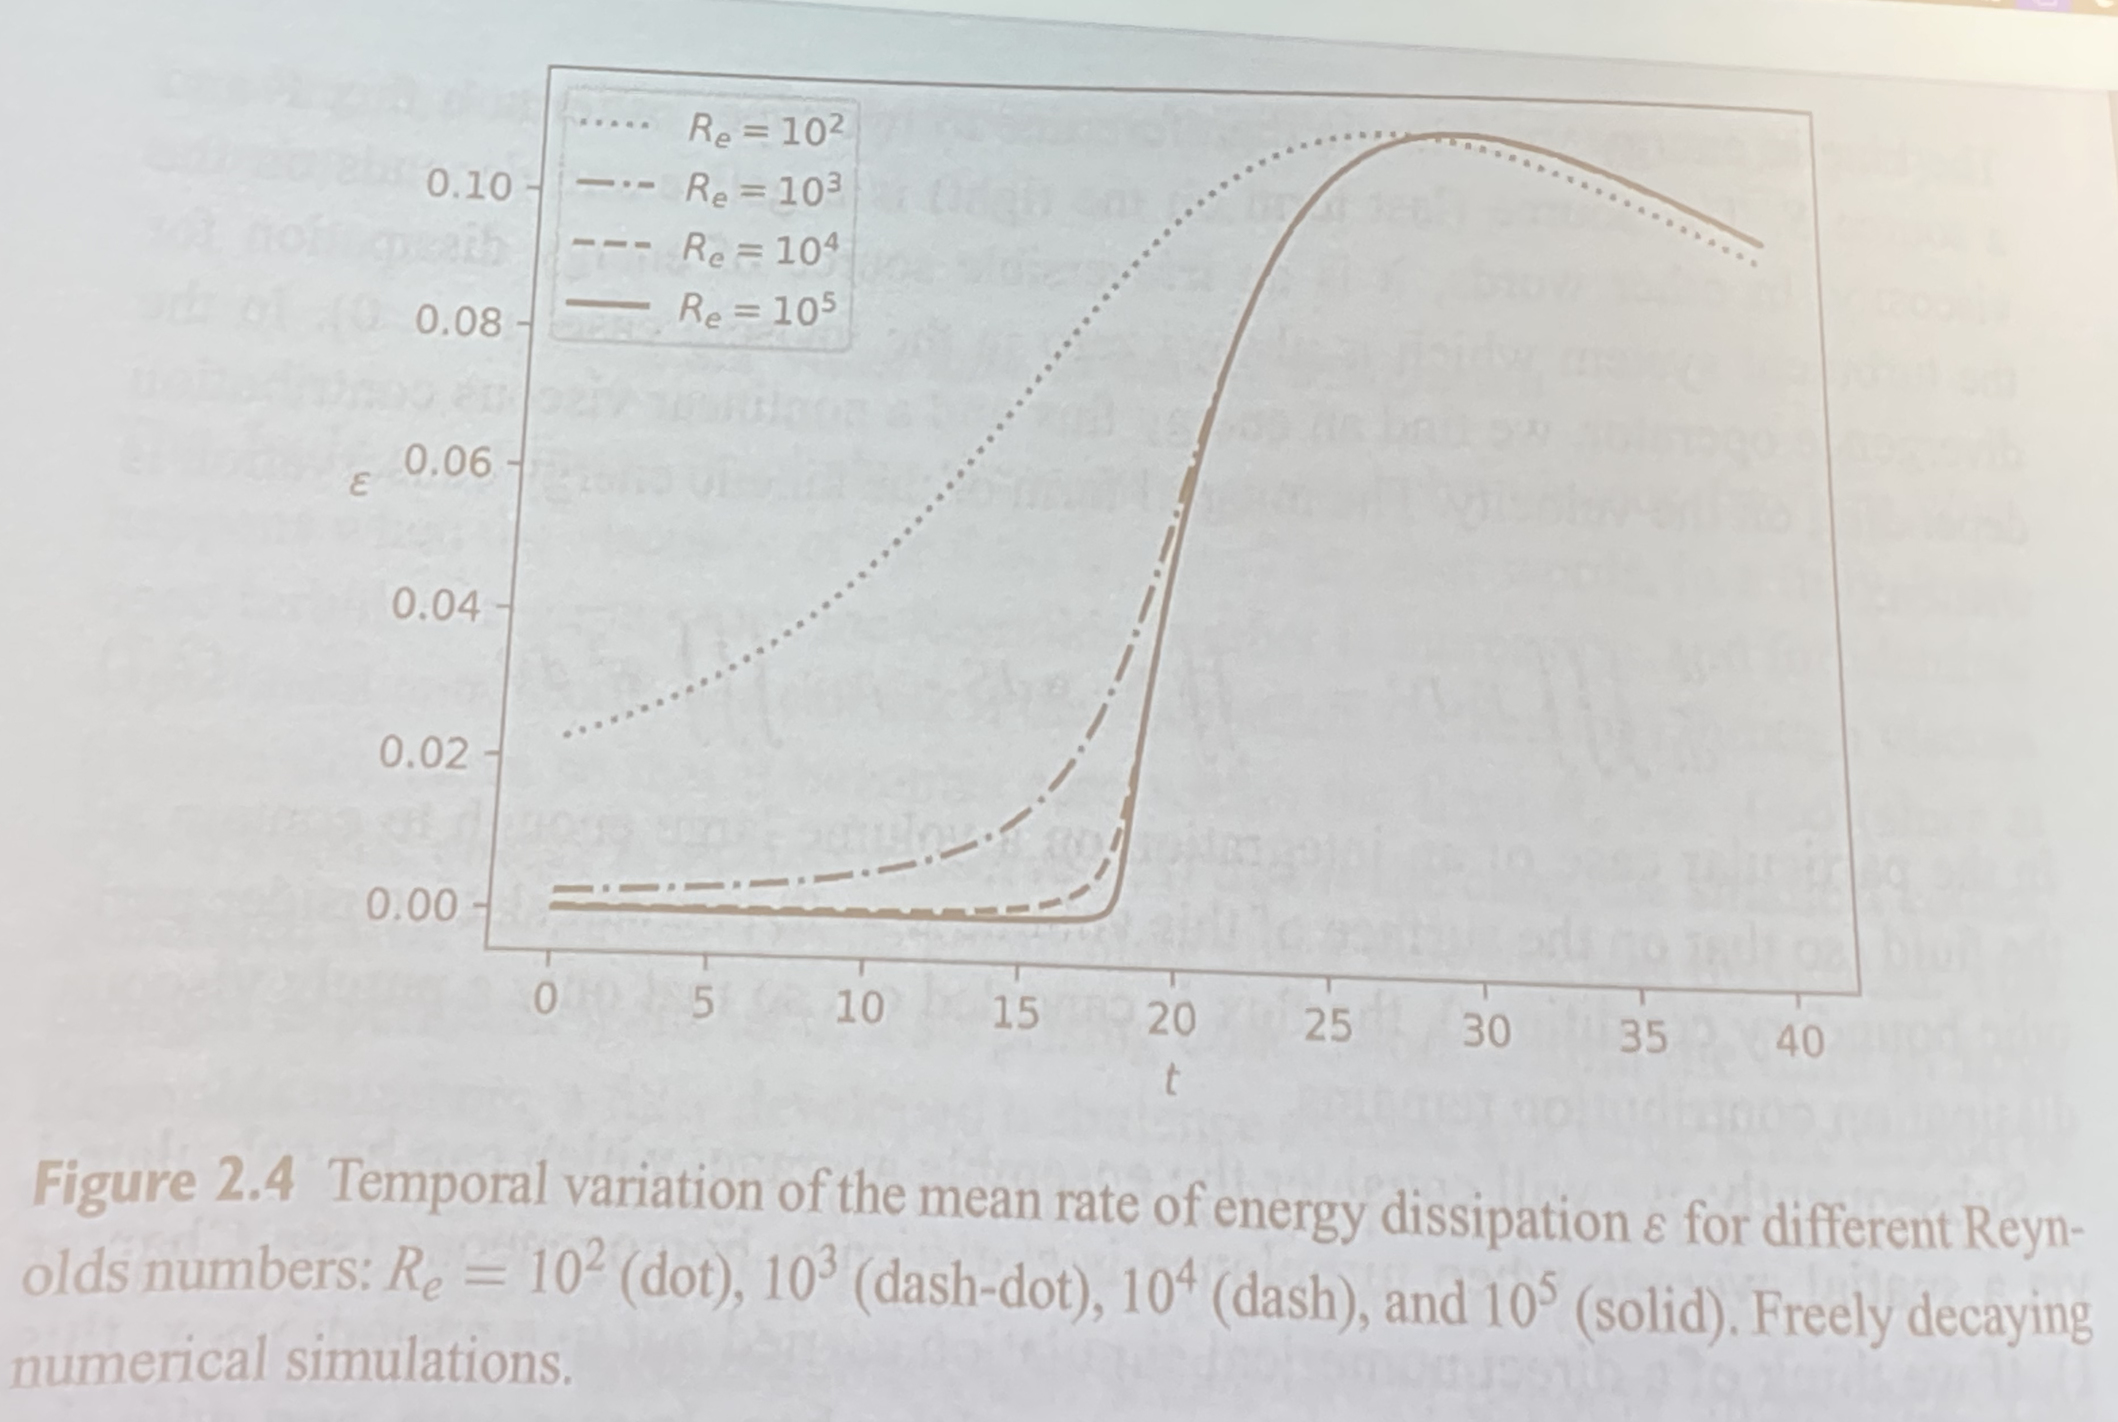
\includegraphics[scale=0.2]{Lectures/Images/lec13-eRecurves.png}
\end{center}

Next time, we will show that the enstrophy, together with the energy, are conserved quantities in two dimensions. Then, we will show that if we add in odd viscosity, that 3D flows look like 2D. Then, we will look at how odd viscosity changes the 2D turbulent cascade, and then also the 3D turbulent cascade as a result of quasi-2D-behaviour.
\section{Turbulence III}
Today we discuss turbulence in 2D. Under some conditions, we can approximate the Earth's atmosphere as a thin layer of fluid, or we can consider a fluid interface etc. To this end, we start by studying turbulence in 2D systems.

\subsection{Vorticity and Enstrophy}
Recall the Enstrophy\footnote{``I just had a rant that we don't use $Z$ (the partition function) in the class, but now it's back.... revenge of the $Z$''}:
\begin{equation}
    Z = \int d^d\v{x}(\nabla \times \v{v})^2
\end{equation}
with $d = 2$ and $\nabla \cdot \v{v} = 0$ (incompressability). The curl of the velocity field is the vorticity:
\begin{equation}
    \gv{\omega} = \nabla \times \v{v}
\end{equation}
Writing down the Navier-Stokes equation:
\begin{equation}
    \p_t \v{v} + \v{v} \cdot \nabla \v{v} = -\frac{1}{\rho}\nabla p + \nu \nabla^2\v{v}
\end{equation}
Now taking the curl of this equation (the pressure term drops out as the curl of a gradient is zero):
\begin{equation}
    \p_t \gv{\omega} + \nabla \times (\v{v} \cdot \nabla \v{v}) = \nu \nabla^2 \gv{\omega}
\end{equation}
To work on the second term, we consider the identity:
\begin{equation}
    \nabla(\v{u} \cdot \v{v}) = (\v{u} \cdot \nabla)\v{v} + (\v{v} \cdot \nabla)\v{u} + \v{u} \times (\nabla \times \v{v}) + \v{v}\times (\nabla \times \v{u})
\end{equation}
and in particular taking $\v{u} = \v{v}$:
\begin{equation}
    \nabla(\frac{1}{2}\abs{\v{v}}^2) = \v{v} \cdot \nabla \v{v} + \v{v} \times (\nabla \times \v{v})
\end{equation}
Thus:
\begin{equation}
    \nabla \times (\v{v} \cdot \nabla \v{v}) = \nabla \times (\nabla\left(\frac{v^2}{2}\right)) - \nabla \times (\v{v} \times \gv{\omega}) = \nabla \times (\gv{\omega} \times \v{v})
\end{equation}
where we have used again that the curl of a gradient is zero. Expanding out this last term:
\begin{equation}
    \nabla \times (\v{v} \cdot \nabla \v{v}) = (\v{v} \cdot \nabla)\gv{\omega} - (\gv{\omega}\cdot\nabla)\v{v} + \gv{\omega}(\nabla \cdot \v{v}) + \v{v}(\nabla \cdot \gv{\omega})
\end{equation}
The third term drops out because we assume the fluid is incompressible. The fourth term drops out because the divergence of a curl ($\gv{\omega}$ is a curl of $\v{v}$) is zero. Hence:
\begin{equation}
    \nabla \times (\v{v} \cdot \nabla \v{v}) = (\v{v} \cdot \nabla)\gv{\omega} - (\gv{\omega}\cdot\nabla)\v{v}
\end{equation}
So the Navier Stokes equation becomes:
\begin{equation}
    \p_t \gv{\omega} + (\v{v} \cdot \nabla)\gv{\omega} = (\gv{\omega} \cdot \nabla)\v{v} + \nu\nabla^2\gv{\omega}
\end{equation}
The object on the LHS is a total derivative, so let us write it this way. Further, for any 2D system, $\gv{\omega}$ points out of the plane while $\nabla$ exists in the plane, so $\gv{\omega}\cdot\nabla = 0$. Hence:
\begin{equation}
    \dod{\gv{\omega}}{t} = \nu \nabla^2\gv{\omega}
\end{equation}
Further, if we take the limit where the viscosity vanishes (e.g. the inertial range of the turbulent cascade), then:
\begin{equation}
    \dod{\gv{\omega}}{t} = 0
\end{equation}
Hence under our set of assumptions, $\gv{\omega}$ is conserved! The only way to not conserve it is to switch on a dissipation $\nu$. Any function of $\gv{\omega}$ is conserved, and hence $\gv{\omega}^2$ - the entstrophy density, and the total enstrophy, are both conserved. So in 2D, in addition to the energy, the enstrophy is also a conserved quantity. The question then becomes - can we have turbulent cascades in this setting? What are the consequences of conservation?

\subsection{Turbulence in 2D - Dual Cascade}
We can write the energy per unit area as:
\begin{equation}
    E = \frac{\text{Energy}}{\text{Area}} = \frac{1}{2}\avg{\v{v}^2} = \int E(k)dk
\end{equation}
we can write down an analogous expression for the enstrophy:
\begin{equation}
    Z = \frac{\text{Enstrophy}}{\text{Area}} = \frac{1}{2}\avg{\gv{\omega}^2} = \int k^2E(k)dk
\end{equation}
where we got the last expression by recalling that $\gv{\omega} = \nabla \times \v{v}$ and so $\gv{\omega}_\v{\v{k}} = i\v{k} \times \v{v}_{\v{k}}$. We can also look at the dissipated power:
\begin{equation}
    P = \nu \int d^d\v{x}(\p_i v_j)^2 \stackrel{\text{FT}}{\to} \nu k^2E(k)
\end{equation}

Now we ask - how do $E, Z$ cascade? They show a dual cascade behaviour, as shown by Fjørtoft in 1953. In $k$-space, the spectral density of $Z$ is related to the energy spectrum via $Z_k = k^2E(k)$ as we found above. Fjørtoft invites us to consider the following setup. We inject energy at $k_f$, in a band of size $\Delta_f$. In this range $\text{Re} \gg 1$ so no dissipation can occur. We consider a small and large $k_{d_1}, k_{d_2}$ where dissipation can occur. In between is the inertial range.

\begin{center}
    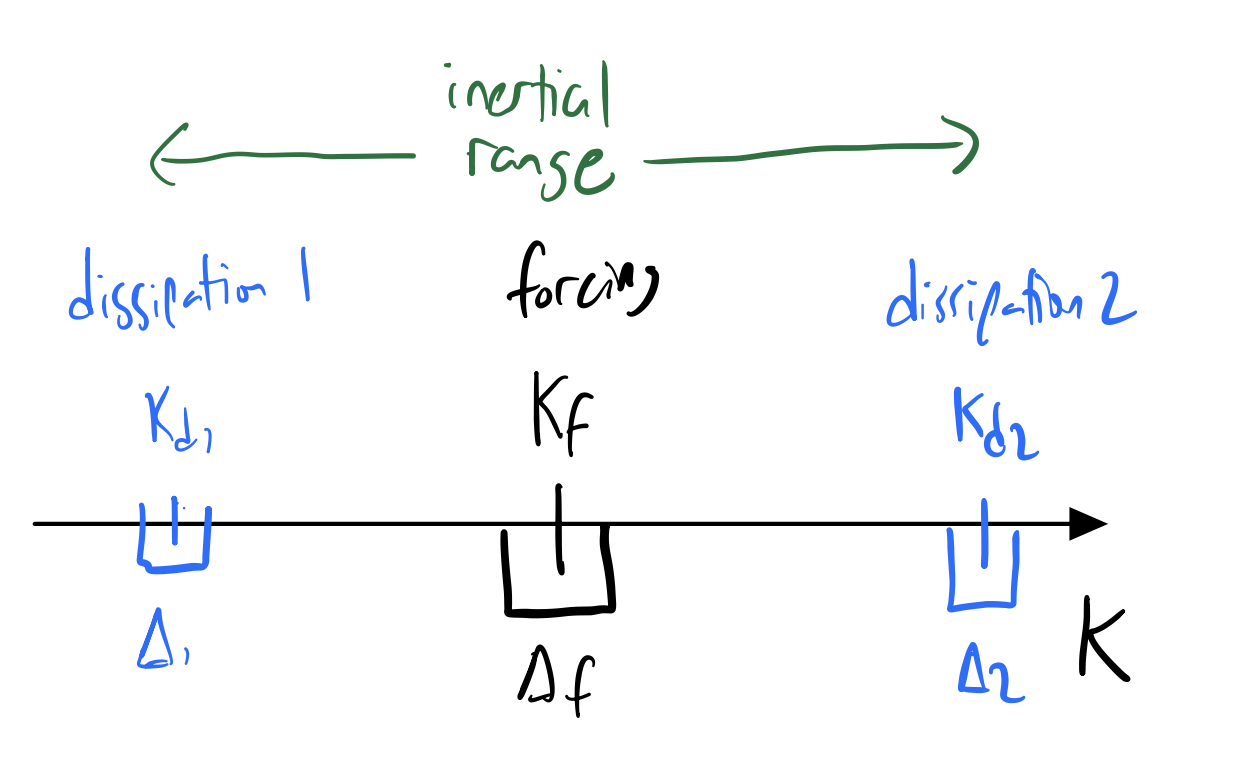
\includegraphics[scale=0.35]{Lectures/Images/lec14-kscale.png}
\end{center}

\begin{enumerate}
    \item Let us suppose that in range $\Delta_f$ around $k_f$ we produce energy per unit time of $\e$. This amounts to a respective rate of enstrophy production:
    \begin{equation}
        \eta = k_f^2\e
    \end{equation}
    \item Now, we construct a \emph{reductio ad absurdum}/proof by contradiction. Suppose now that a comparable amount of energy $\e$ is dissipated per unit time near $k_{d_2}$. This corresponds to a respective rate of enstrophy dissipation:
    \begin{equation}
        \eta' = k_{d_2}^2\e \gg k_f^2\e = \eta
    \end{equation}
    This is not possible in a steady state (i.e. it is not possible to dissipate $Z$ as a rate larger than the rate of production, as enstrophy is conserved). Thus we conclude most of the energy must be dissipated at the other end of the spectrum, near $k_{{d_1}}$.
    \item Similarly, assuming dissipation of $Z$ near $k_{d_1}$ at a rate $\eta$ also leads to a contradiction, as we dissipate $E$ at a rate:
    \begin{equation}
        \e' = \left(\frac{1}{k_{d_1}}\right)^2\eta \gg \left(\frac{1}{k_f}\right)^2\eta = \e
    \end{equation}
    \textcolor{red}{(Partially missed this part, so this argument may not quite be correct. I also didn't quite get the punchline of what we conclude from the proofs of contradiction.)}
\end{enumerate}

\begin{center}
    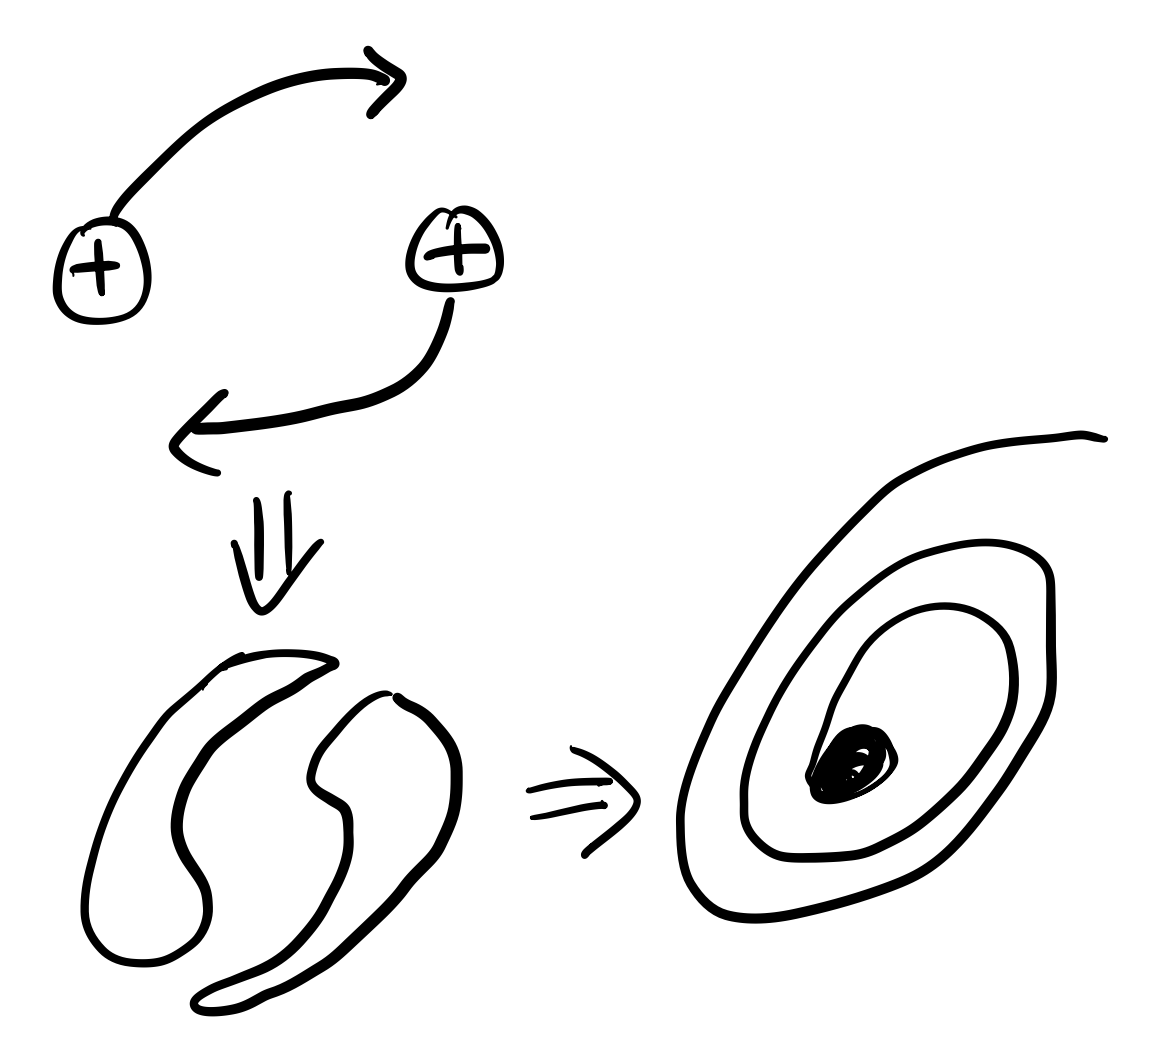
\includegraphics[scale=0.35]{Lectures/Images/lec14-vortexmerger.png}
\end{center}

What happens is we have 2D vortex mergers (two vortices of scale $L$ go to scale $2L$), where energy goes into the vortex core, while enstrophy goes into thin filaments. Simultaneously to this, there is a direct cascade of the enstrophy. This is the notion of the dual cascade in real space - concentration of enstrophy in the filaments, and the concentration of energy in the large-scale vortex cores.

What we will do next time - using the same dimensional analysis argument (a la Kolmogorov) we did in 3D to find the power spectrum in 2D. Since the enstrophy density has a $k^2$, we will see that it has a different power law. Then, we will see how even in 3D under the presence of odd viscosity we have quasi-2dimensionalization.
\section{Turbulence IV}

\subsection{Review: The double cascade}

\begin{center}
    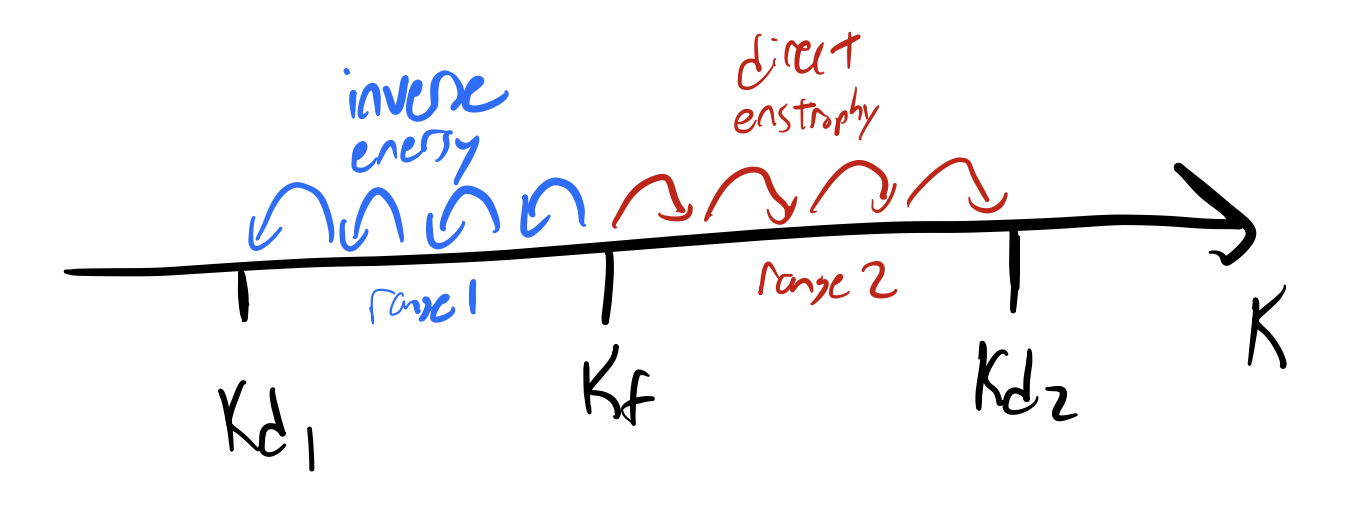
\includegraphics[scale=0.4]{Lectures/Images/lec15-dualcascade.png}
\end{center}

Between $k_{d_1}$ and $k_{d_2}$, we have an inertial regime with no dissipation. We considered two scenarios where we injected energy at $k_f$. Then we found that there is an inverse energy cascade towards $k_{d_1}$ and a direct enstrophy cascade towards $k_{d_2}$. The enstrophy was defined as the integral of vorticity:
\begin{equation}
    Z = \int \gv{\omega}^2 d^2\v{x}.
\end{equation}

The argument was derived by Kraichnan 1967, who started looking at nonlinear PDEs by studying gravity at IAS with Einstein. He then turned to turbulence, and did the rest of his academic career as a hermit living in a cabin in New Hampshire.

\subsection{Power Spectrum Derivation}
We now have the direction of the cascade - let us now figure out the power spectrum, in the same way that we derived the power spectrum for the energy cascade in the Kolmogorov argument.

Note that there is an important implicit assumption, namely that of locality (in $k$-space). More precisely, we assume that non-local energy transfer between far-away $k$ values is not possible, and hence the spectrum in range 1 only depends on the the rate of energy injection $\e$, and the spectrum in range 2 only depends only on the rate of enstrophy production $\eta$. Hence, in $k$-space we can treat the two problems as independent. Note that $\eta = k^2\e$ so we are not saying that there is only energy or enstrophy in one of the two regimes, just that there is a dominant process (and hence energy spectrum power law) in each regime.

First, let's look at the dimensionality of $\eta$:
\begin{equation}
    [\eta] = \frac{[\text{enstrophy density}]}{[\text{time}]} = \frac{[\gv{\omega}^2]}{[t]} = \frac{[(\nabla \times \v{v})^2]}{[t]} = \frac{\left(\frac{1}{[t]}\frac{[L]}{[t]}\right)^2}{[t]} = \frac{1}{[t]^3}
\end{equation}
The dimensionality of $E_k$ (power spectrum of energy) is:
\begin{equation}
    [E_k] = \frac{[l]^3}{[t]^2}
\end{equation}
So we want a relation:
\begin{equation}
    E_k = c_2\eta^{\alpha}k^{\beta}
\end{equation}
$\eta$ provides the time dependence, $k$ provides the spatial dependence, so:
\begin{equation}
    E_k = c_2\eta^{2/3}k^{-3}
\end{equation}
The argument for the direct cascade we did a couple lectures ago (Kolmogorov '41) yielded:
\begin{equation}
    E_k = c_1\e^{2/3}k^{-5/3}
\end{equation}
so we have two power laws, which dominate in different regimes.

\subsection{Turbulence + Odd Viscosity}
We now want to study what happens when we add odd viscosity - e.g. a rotating box/atmosphere, or individually rotating particles. This leads to a quasi-2-dimensionalization of the fluid flow.

In 3D we would expect to have a picture where we have a soup\footnote{You shouldn't eat it.} of vortices in 3D which is scale invariant in the cascading regime. What we will see happen is that we still will have many vortices, but they will be roughly aligned along the direction $\hat{\gv{\Omega}}$ of rotation.

\begin{center}
    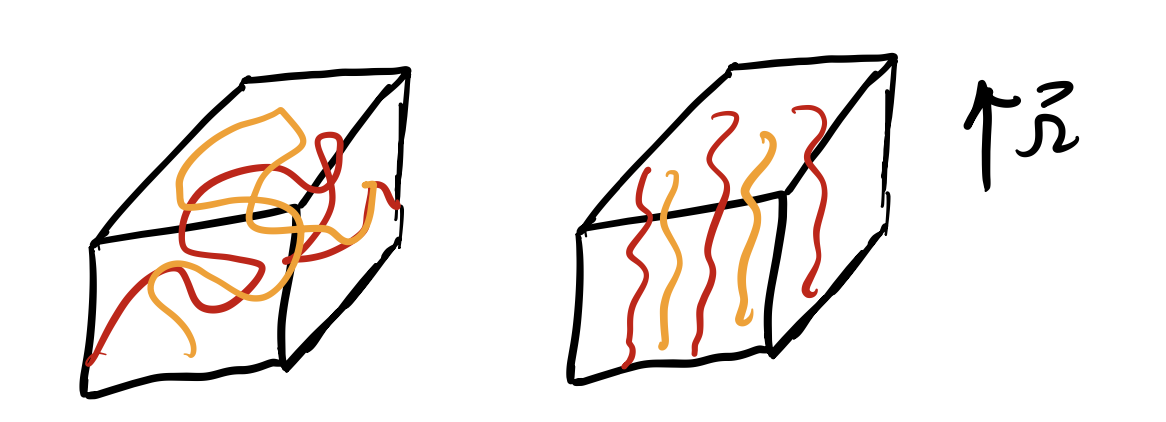
\includegraphics[scale=0.4]{Lectures/Images/lec15-vortices.png}
\end{center}

Let's return to the Navier-Stokes equation, adding a rotation term
\begin{equation}
    \p_t \v{v} + \v{v} \cdot \nabla \v{v} = -\frac{1}{\rho_0}\nabla p + \nu\nabla^2\v{v} + \begin{cases}
        \Omega \hat{\v{z}} \times \v{v} & \text{Coriolis} \\ \nu^0 \hat{\v{z}} \times \nabla^2 \v{v} & \text{Odd Viscosity}
    \end{cases}
\end{equation}
with $\nu = \eta/\rho$. Notice that, comparing the two cases, we can interpret odd viscosity as a length scale dependent coriolis force $\sim \Omega v \nu^0 k^2$.

\subsection{Taylor-Proudman Argument}
The following argument is presented by Proudman and G.I. Taylor, who is famous for estimating the energy of the Trinity nuclear test to the correct order of magnitude. 

We have two dimensionless parameters of interest; the Reynolds number $\text{Re} = \frac{VL}{\eta}$ and the odd viscosity ratio $\frac{\nu^0}{\nu}$. The $\frac{\nu^0}{\nu} \ll 1$ case is ``simple'', we can drop the $\nu^0$ term and then this is just isotropic viscosity, and we already know the power spectrum to be $\sim k^{-5/3}$ (this the Kolmogorov regime). The interesting limit is $\frac{\nu^0}{\nu} \gg 1$. The argument relies on a balance between two terms, the pressure and the rotational term. We neglect the $\v{v} \cdot \nabla \v{v}$ term - this is ok for low Reynolds, but is problematic at high Reynolds.

Let's look at the argument for the odd viscosity case. The balance of the term gives us:
\begin{equation}
    \eta^0 \hat{\v{z}} \times \nabla^2\v{v} = \nabla p
\end{equation}
Let us now take a curl on both sides, wherein the pressure term vanishes (curl of grad is zero). Now, we use the identity:
\begin{equation}
    \nabla \times (\v{F} \times \v{G}) = \v{F}\nabla \cdot \v{G} - \v{G}\nabla \cdot \v{F} + (\v{G} \cdot \nabla)\v{F} - (\v{F}\cdot\nabla)\v{G}
\end{equation}
where we have $\v{F} = \zhat$ and $\v{G} = \nabla^2\v{v}$. Since $\zhat$ is a constant, the derivative terms of $\zhat$ vanish (so the second/third terms drop out). Further, the first term drops out as:
\begin{equation}
    \nabla \cdot (\nabla^2\v{v}) = \nabla^2(\nabla \cdot \v{v}) = 0
\end{equation}
from incompressibility. Hence we are left with:
\begin{equation}
    \eta^0(\zhat \cdot \nabla)\nabla^2\v{v} = 0 \implies  \nabla^2\p_z\v{v} = 0
\end{equation}
This tells us that:
\begin{equation}
    \boxed{\p_z \v{v} \approx \v{0}}
\end{equation}
This is the sense that we believe that there might be quasi-2-dimensionalization.

\subsection{Regimes of Turbulence}
This was a fairly simple and approximate argument. But, one thing we can do is also simulate the Navier-Stokes equations with the odd viscosity term, and observe what we see. 

\begin{center}
    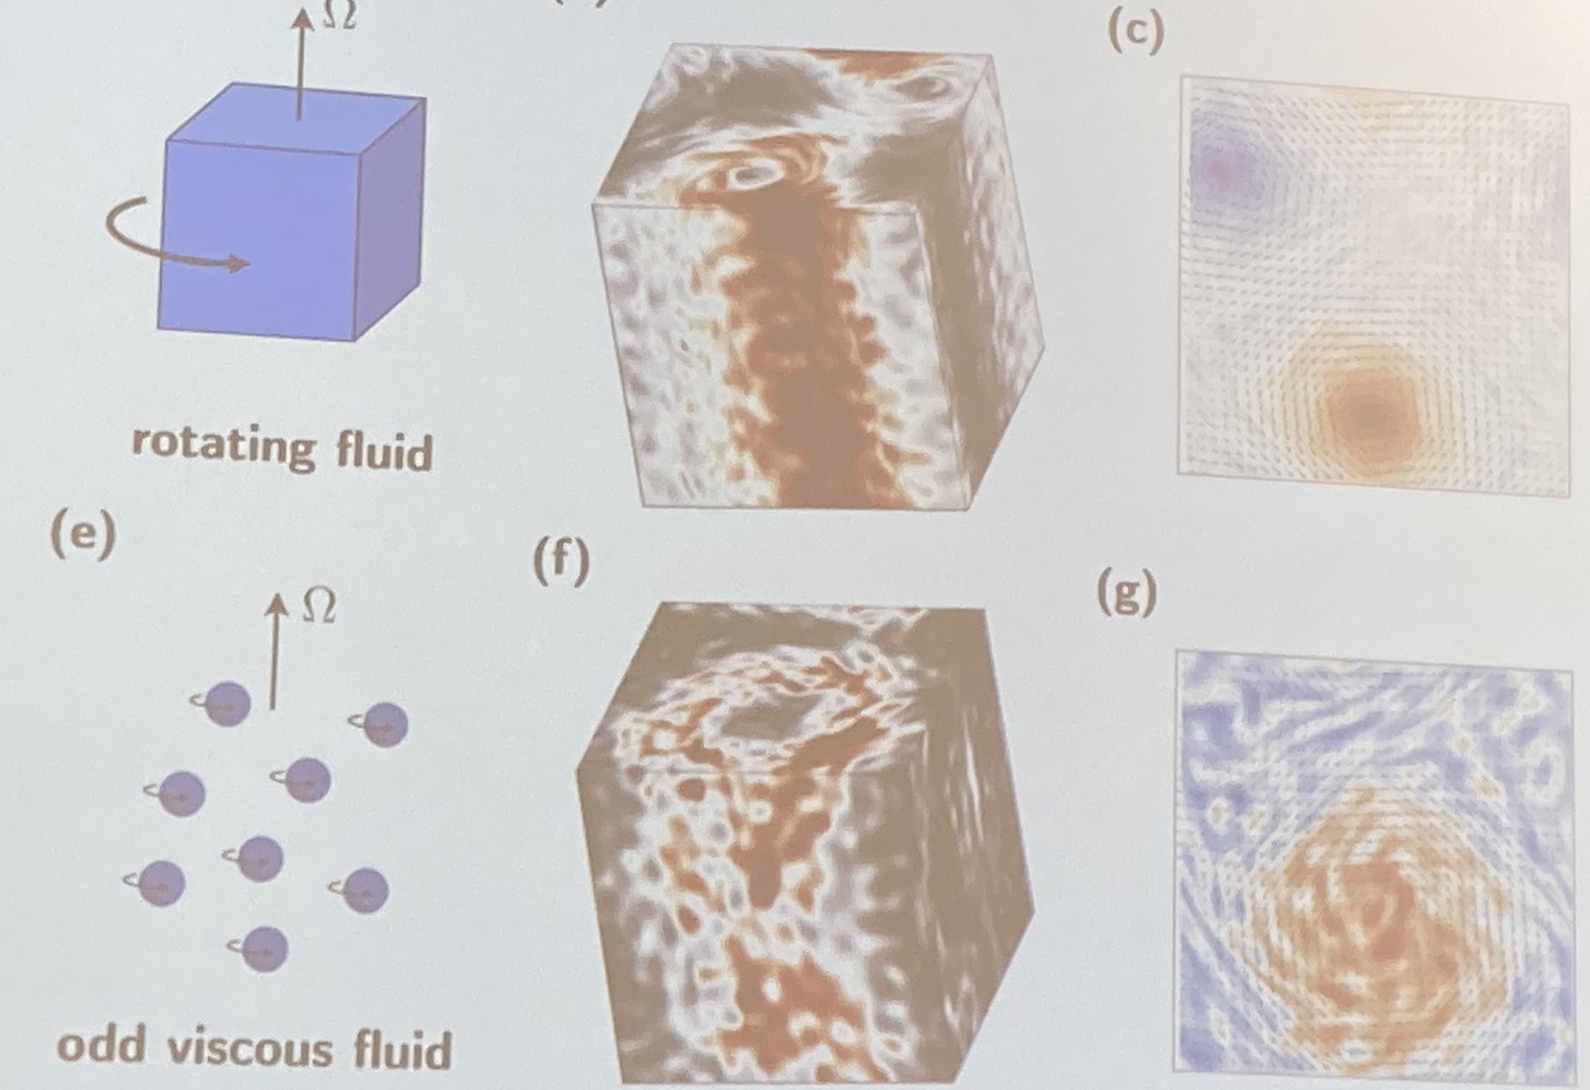
\includegraphics[scale=0.4]{Lectures/Images/lec15-simulation.png}
\end{center}

We notice that for the most part, we have a column vortex in the $\zhat$ direction\footnote{Why is the quasi-2-dimensionalization harder to see in the odd viscous fluid case? We have to go to high $k$ so that the odd viscosity effect is important. There's a subtlety because the vortices are on the length scale of the box, while they are caused by small-scale physics (rotating particles), so there is a lot of information to retain - it (unlike the Coriolis/body force case) is a multiscale problem.}, which is what the Taylor-Proudman argument hints at. But this simulation is done in a regime where the $\v{v} \cdot \nabla \v{v}$ term is kept - there are mathematical arguments that nonlinearities introduced by this term do not spoil the quasi-2-dimensionalization.

Note that when comparing the rotating fluid and odd viscosity case, we have the $k^2$ length-scale dependence. If $k$ is very small (no matter how large $\nu^0$ is) then the odd viscosity term drops out and we just have Kolmogorov turbulence, with a forward energy cascade and energy spectrum that scales as $\sim k^{-5/3}$. At large $k$ the odd viscosity term becomes important, and we have quasi-2-dimensionalization, wherein we have an inverse cascade. The two asymptotic regimes are separated by a characteristic inverse wavelength $k_{\text{odd}}$ representing the crossover between the two regimes. So, there are two things to try to find - the power spectrum scaling as well as the crossover wavelength (and what happens in this regime).

\begin{center}
    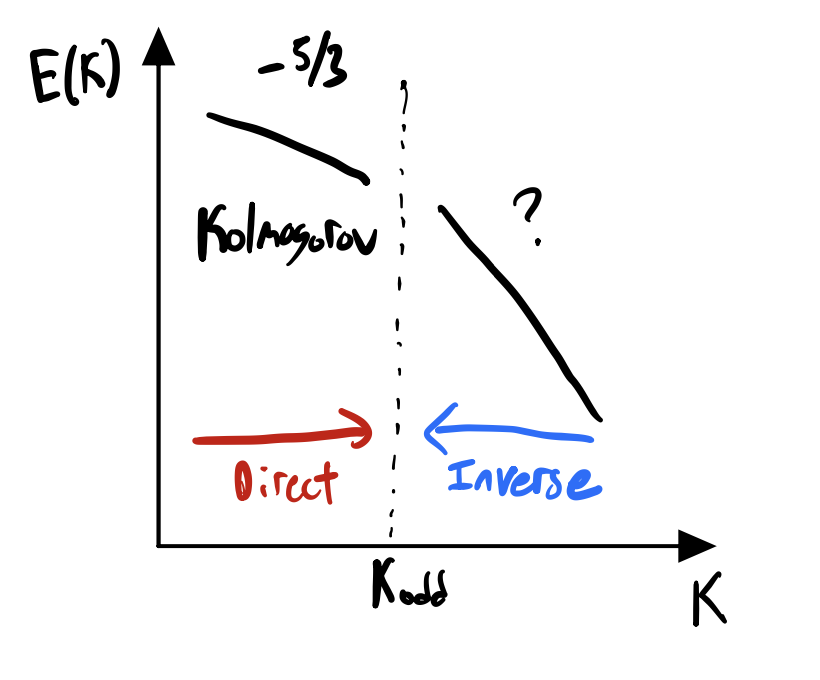
\includegraphics[scale=0.4]{Lectures/Images/lec15-oddpowerspectrum.png}
\end{center}

It is interesting to compare this with the Kraichnan argument, where we have an outward flux of energy/enstrophy away from $k_f$, vs. here where we have an inward flux of energy towards $k_{\text{odd}}$. In $k$-space we expect a sharp peak at $k_{\text{odd}}$ which suggests that there is a periodic behaviour of the system in real space.

One thing we can say is that $k_{\text{odd}} \sim f(\nu^0)$, because $\nu^0 = 0$ then $k_{\text{odd}}$ would be infinity (we would just have the Kolmogorov turbulence at all scales).

Let's start by estimating the power spectrum power law (we make the physical assumption that $\e$ is linear in the characteristic time $\tau$ - this is not physically obvious)
\begin{equation}
    \e = A\tau k^\alpha E^\beta(k)
\end{equation}

We know that $[\tau] = t$, $[\e] = \frac{l^2}{t^3}$ and $[E(k)] = \frac{l^3}{t^2}$. So:
\begin{equation}
    [\e] = l^{-\alpha + 3\beta} t^{-2\beta + 1} \implies l^2 t^{-4} = l^{-\alpha + 3\beta}t^{-2\beta}
\end{equation}
hence:
\begin{equation}
    2 = 3\beta - \alpha
\end{equation}
\begin{equation}
    -4 = -2\beta
\end{equation}
which is solved by:
\begin{equation}
    \beta = 2, \alpha = 4
\end{equation}

So by dimensional analysis, we find:
\begin{equation}
    \boxed{\e = A\tau(k)k^4 E^{2}(k)}
\end{equation}
which tells us that if we know the characteristic time scale of our process and the power spectrum, we know the energy transfer rate. We can then invert this to obtain an equation of the power spectrum in terms of $\e, \tau, k$. If we put the Eddy turnover time in for $\tau$ then we get the Kolmogorov result, and we will make an appropriate modification for the odd turbulence case.

For more detail, you may refer to \texttt{De Wit, Fruchart, Khain, Toschi, Vitelli, \emph{Nature 2024}}.


Next time, we will also study how linear stability analysis can be used to study pattern formation. This is something we will look at next lecture. What is very interesting to note here is that we have a very different mechanism of pattern formation, via energy cascades from turbulence (highly nonlinear)! 
\section{Turbulence V}
Since the last problem set is quite long and close to the end of the quarter, the remaining lectures will be sketching out the problems, and you will have the task of filling out the steps.

\subsection{Review}
Let us write the starting point of all of our travels/joy:
\begin{equation}\label{eq:NSwithoddviscos}
    \p_t \v{v} + \v{v} \cdot \nabla \v{v} = -\frac{1}{\rho_0}\nabla p + \nu \nabla^2\v{v} + \nu_0\zhat \times \nabla^2\v{v}
\end{equation}
in the homework you actually take this one step further and consider two odd viscosities. In 2D, we can impose isotropy; we can make the particles spin in the plane, with rotation axis perpendicular to the plane. In 3D, the rotation axis must live in the space, so we can have the possibility of more terms. This is all to say - the model we have been studying in lecture we have taken the liberty of simplifying a little bit, in the interest of not writing down an excessive amount of terms (even though in real materials we of course have a lot of terms - but the statistical mechanical features of many realistic models are captured with simpler models, e.g. modelling magnets via the Ising model).

The last term in Eq. \eqref{eq:NSwithoddviscos} corresponds to the odd viscosity term. We could also consider instead a term $\Omega\zhat \times \v{v}$ corresponding to a Coriolis/body force - odd viscosity is like considering a $k$-dependent Coriolis force of $\Omega \sim \nu^0 k^2$.

We looked at the Taylor-Proudman argument, where we balanced the pressure term and the chiral term, and found that:
\begin{equation}
    \p_z \v{v} \approx 0
\end{equation}
i.e. the chiral term seems to make the 3D system quasi-2D. We saw this in simulations as well, where the vortices in the fluid aligned along the rotation axis.

We also thought about the energy spectrum - for small $k$ we have the Kolmogorov direct cascade, and for large $k$, large $\frac{\nu^0}{\nu} \gg 1$ (and of course $\text{Re} \gg 1$ throughout) we have quasi-2-dimensionalization and get an inverse energy cascade.

\begin{center}
    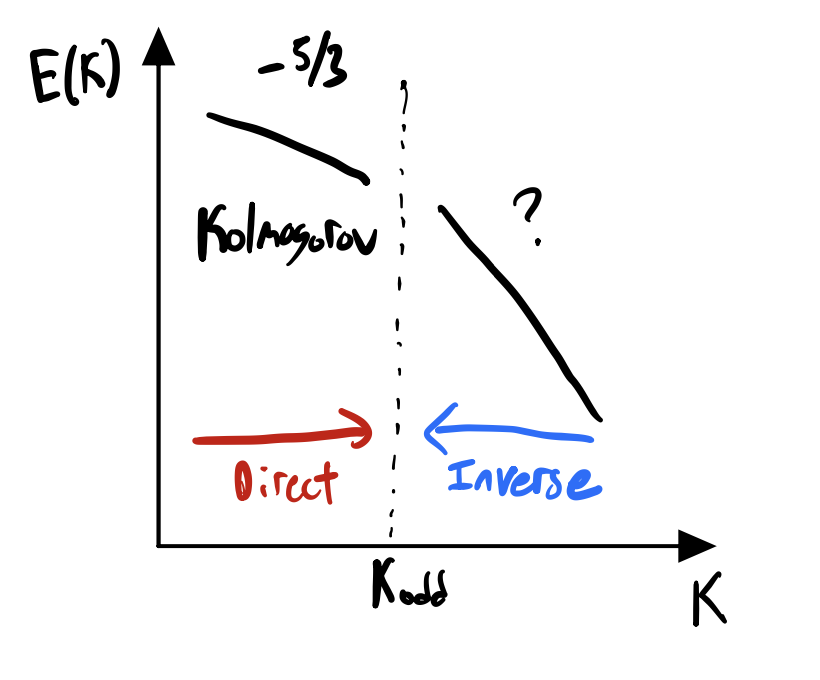
\includegraphics[scale=0.4]{Lectures/Images/lec15-oddpowerspectrum.png}
\end{center}

Note that we still do not know how to connect the two asymptotic regimes in the transition regime of $k = k_{\text{odd}}$. The flow of energy is towards this intermediate scale, where we see pattern formation. Observing that zero $\nu^0$ results in $k_{\text{odd}} = \infty$, we can postulate $k_{\text{odd}} \sim (\nu^0)^{-\alpha}$. 

So our tasks for today - find the power spectrum power law dependence of high $k$ region, then deduce $k_{\text{odd}}$, and then explore the behaviour near this $k_{\text{odd}}$.

We also deduced the Kraichnan formula:
\begin{equation}
    \e \sim \tau(k) k^4E(k)^2
\end{equation}
assuming that the cascade is local in $k$-space, that energy is conserved away from the energy injection, and that $\e$ is linear in $\tau(k)$ (this last assumption is the trickiest assumption to justify/come to grips with). The power spectrum is:
\begin{equation}
    \boxed{E(k) = \left[\frac{\e}{\tau(k)}\right]^{1/2}k^{-2}}
\end{equation}

\subsection{Finishing the Power Spectrum derivation}
Let's review the Kolmogorov analysis. The eddy turnover time is given as:
\begin{equation}
    \tau_{\text{eddy}} \sim \frac{l_k}{v_k} \sim e^{-1/3}k^{-2/3}
\end{equation}
Thus the power spectrum is given by:
\begin{equation}
    E(k) = \left[\frac{\e}{\tau(k)}\right]^{1/2}k^{-2} \sim \left[\frac{\e}{\e^{-1/3}}\right]^{1/2}\left[k^{2/3}\right]^{1/2}k^{-2} = \boxed{\e^{2/3}k^{-5/3}}
\end{equation}
But now what we want to do is the following. We need a hypothesis about what is happening in the inverse cascade region. We recall:
\begin{equation}
    D_t \v{v} = -\frac{1}{\rho_0}\nabla p + \m{\nu & \nu^0 & 0 \\ -\nu^0 & \nu & 0 \\ 0 & 0 & \nu}\Delta\v{v}
\end{equation}
and how the $\nu^0$ symplectic structure allowed the system to support waves/oscillations.

Thus in addition to eddy dynamics, we have wavelike dynamics. Like we have $\tau_k \sim \frac{l_k}{v_k}$ to be the timescale of the eddys, we also have timescale of waves - the period/frequency of a wave. In your homework, you will prove that in the special limit where there is only one odd viscosity, we have:
\begin{equation}
    \omega \sim \nu^0\abs{\v{k}}k_z \sim \nu^0 k^2
\end{equation}
Hence:
\begin{equation}
    \tau_{\text{wave}} \sim \frac{1}{\omega} \sim k^{-2}
\end{equation}
The regimes where one timescale is much shorter than the other are much more comparatively simple to analyze. The regime where they crossover ($\tau_{\text{wave}} \sim \tau_{\text{eddy}}$) is harder to analyze, and tells us about $k_{\text{odd}}$, because both the wave/eddy timescales depend on $k$. Namely:
\begin{equation}
    \nu^0 k_{\text{odd}}^2 = \e^{1/3}k_{\text{odd}}^{2/3} \implies \boxed{k_{\text{odd}} \sim (\nu^0)^{-3/4}}
\end{equation}
If this is true, there is a regime where $k > k_{\text{odd}}$, then the dominant timescale is that of the waves. If we go the Kraichnan formula and plug in the wave timescale, we get:
\begin{equation}
    \boxed{E(k) \sim \left[\e \nu^0 k^2\right]^{1/2}k^{-2} \sim \e^{1/2}(\nu^0)^{1/2}k^{-1}}
\end{equation}
Note that this $E(k)$ has a different $k$ scaling from the Kolmogorov $k^{-5/3}$ and has a dependence on $\nu^0$, arising from the fact that the odd viscosity creates the waves in the fluid.

Let's consider a plot of the spectrum ratio $E(k)/E_0(k)$:

\begin{center}
    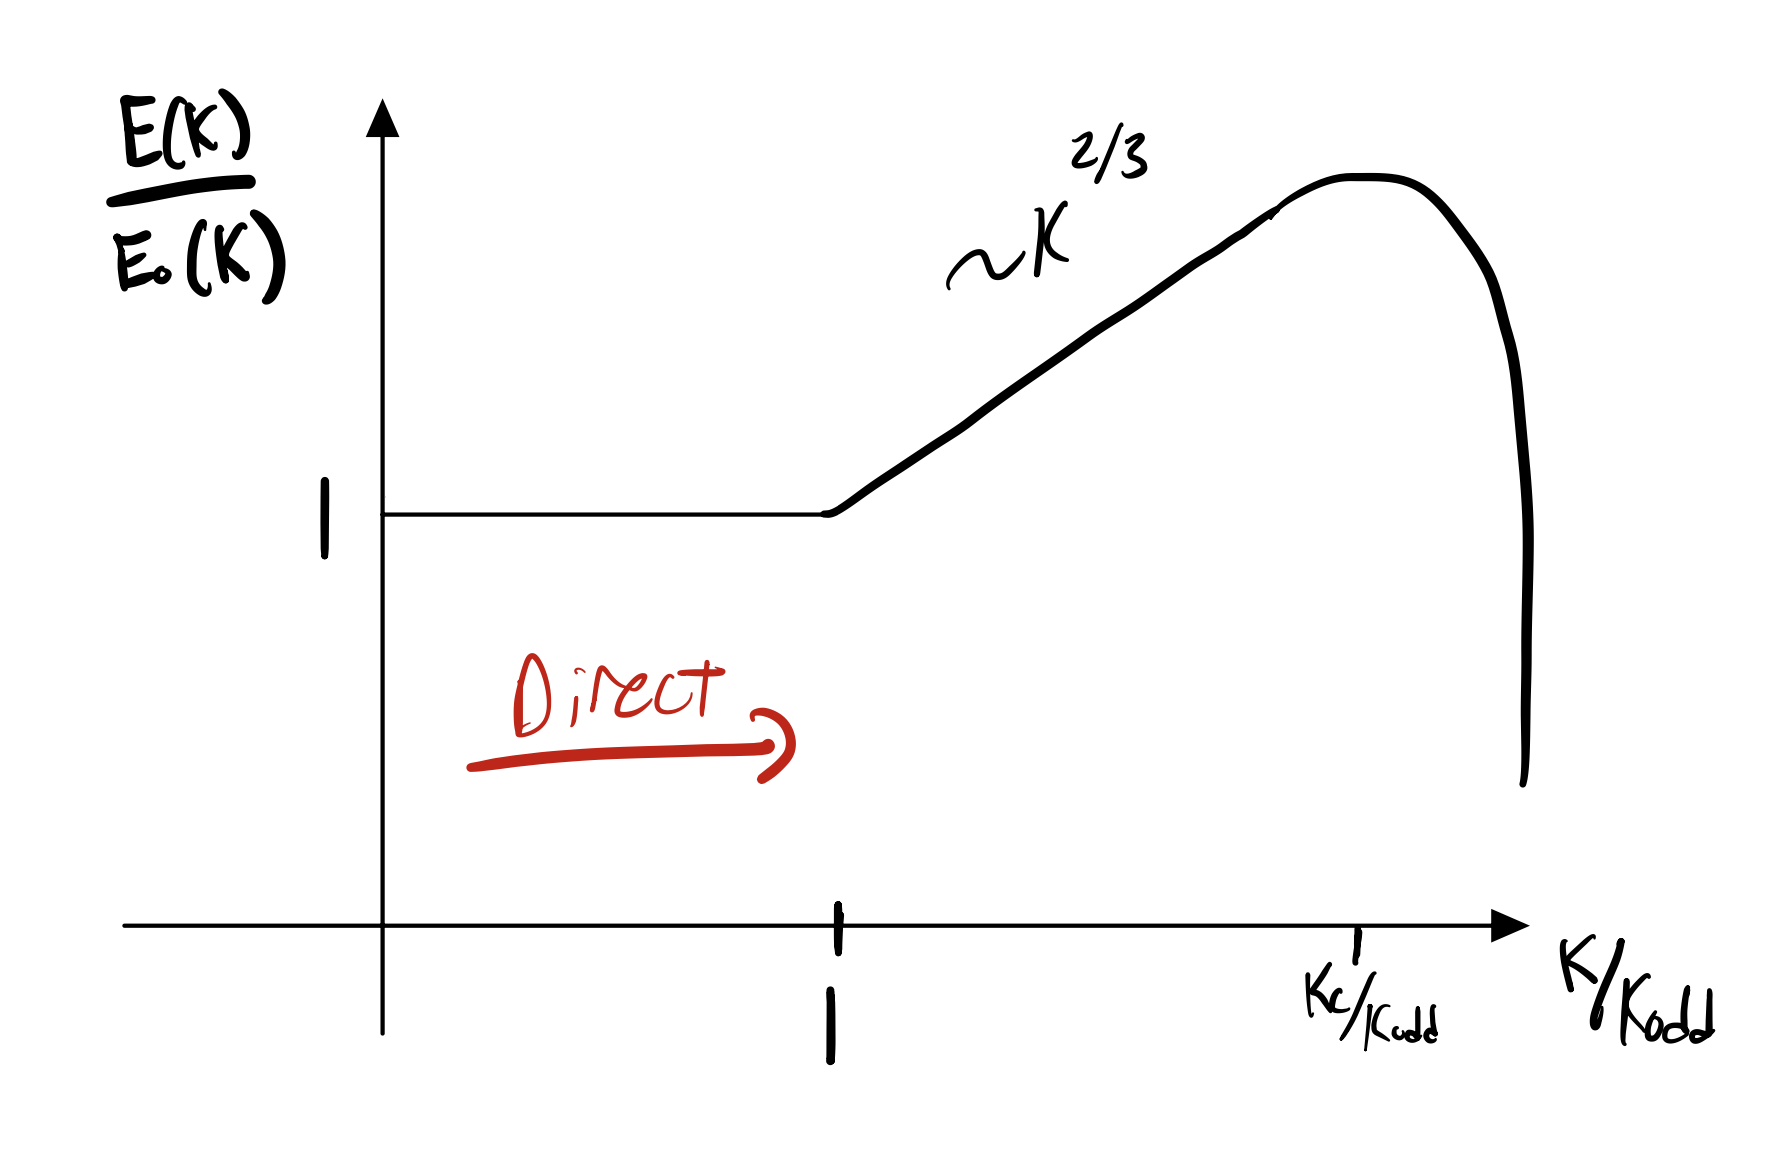
\includegraphics[scale=0.35]{Lectures/Images/lec16-sketch.png}
\end{center}

Where we note that at $k_c$ we have the onset of the dissipative scale. We can estimate this - before, let's look at simulations of a normal fluid $\frac{\nu^0}{\nu} = 0$ and an odd fluid $\frac{\nu^0}{\nu} \gg 1$. In the normal fluid case we see a random distribution of eddys, in the odd viscosity case we see eddy formation on a lengthscale $\sim \frac{1}{k_c}$. We can look at the energy spectrum of such simulations, and we find the structure of Kolmogorov for $k < k_{\text{odd}}$, rising of the power spectrum for $k_{\text{odd}} \leq k \leq k_c$, and the steep dropdown for $k > k_c$.

\begin{center}
    \includegraphics[scale=0.3]{Lectures/Images/lec16-fluidsims.png}
\end{center}


Let us rescale the power spectrum plot above by $k_{\text{odd}}$.

\begin{center}
    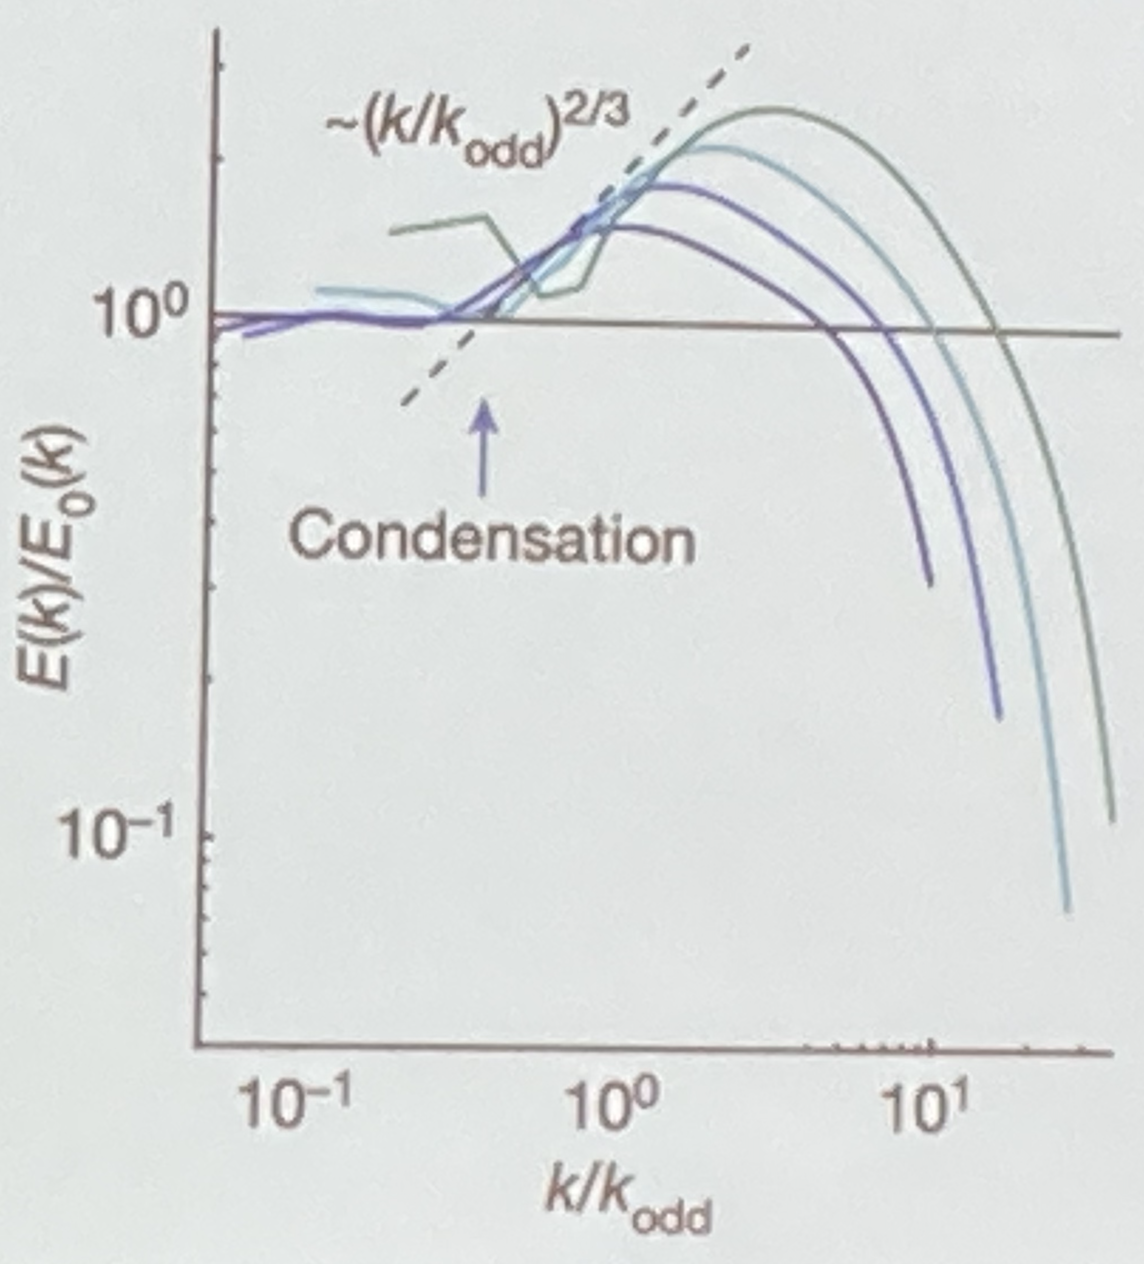
\includegraphics[scale=0.3]{Lectures/Images/lec16-Escaling.png}
\end{center}

We see the curves collapse on one another in the Kolmogorov regime a,d in the $\sim(k/k_{\text{odd}})^{2/3}$ regime, but the maximum shifts, telling us that $k_c$ has some dependence on $\nu^0$ that is different from $k_{\text{odd}}$. Let's see if we can deduce this now. The rate of energy dissipation is given by (coming from $\nu(\nabla \v{v})^2$):
\begin{equation}
    \e_{\text{dis}} \sim \int_{k_{\text{odd}}}^{k_c} \nu k^2 E(k)dk
\end{equation}
Let us carry out this integral:
\begin{equation}
    \e \sim \int_{k_{\text{odd}}}^{k_c}k^2 \e^{1/2}(\nu^0)^{1/2}k^{-1}dk \sim \nu (\nu^0)^{1/2}\e^{1/2}\left.k^2\right|^{k_c}_{k_{\text{odd}}}
\end{equation}
Assuming that $k_c \gg k_{\text{odd}}$ then:
\begin{equation}
    \e \sim \nu (\nu^0)^{1/2}\e^{1/2}k_c^2
\end{equation}
Hence:
\begin{equation}
    \boxed{k_c \sim (\nu^0)^{-1/4}}
\end{equation}
so, if i keep track the initial data of all the maxima of $E(k)/E_0(k)$, we can then plot $k_c$ as a function of $\nu_0/\nu$, and we have evidence for power law scaling of $(\nu^0)^{-1/4}$.

\begin{center}
    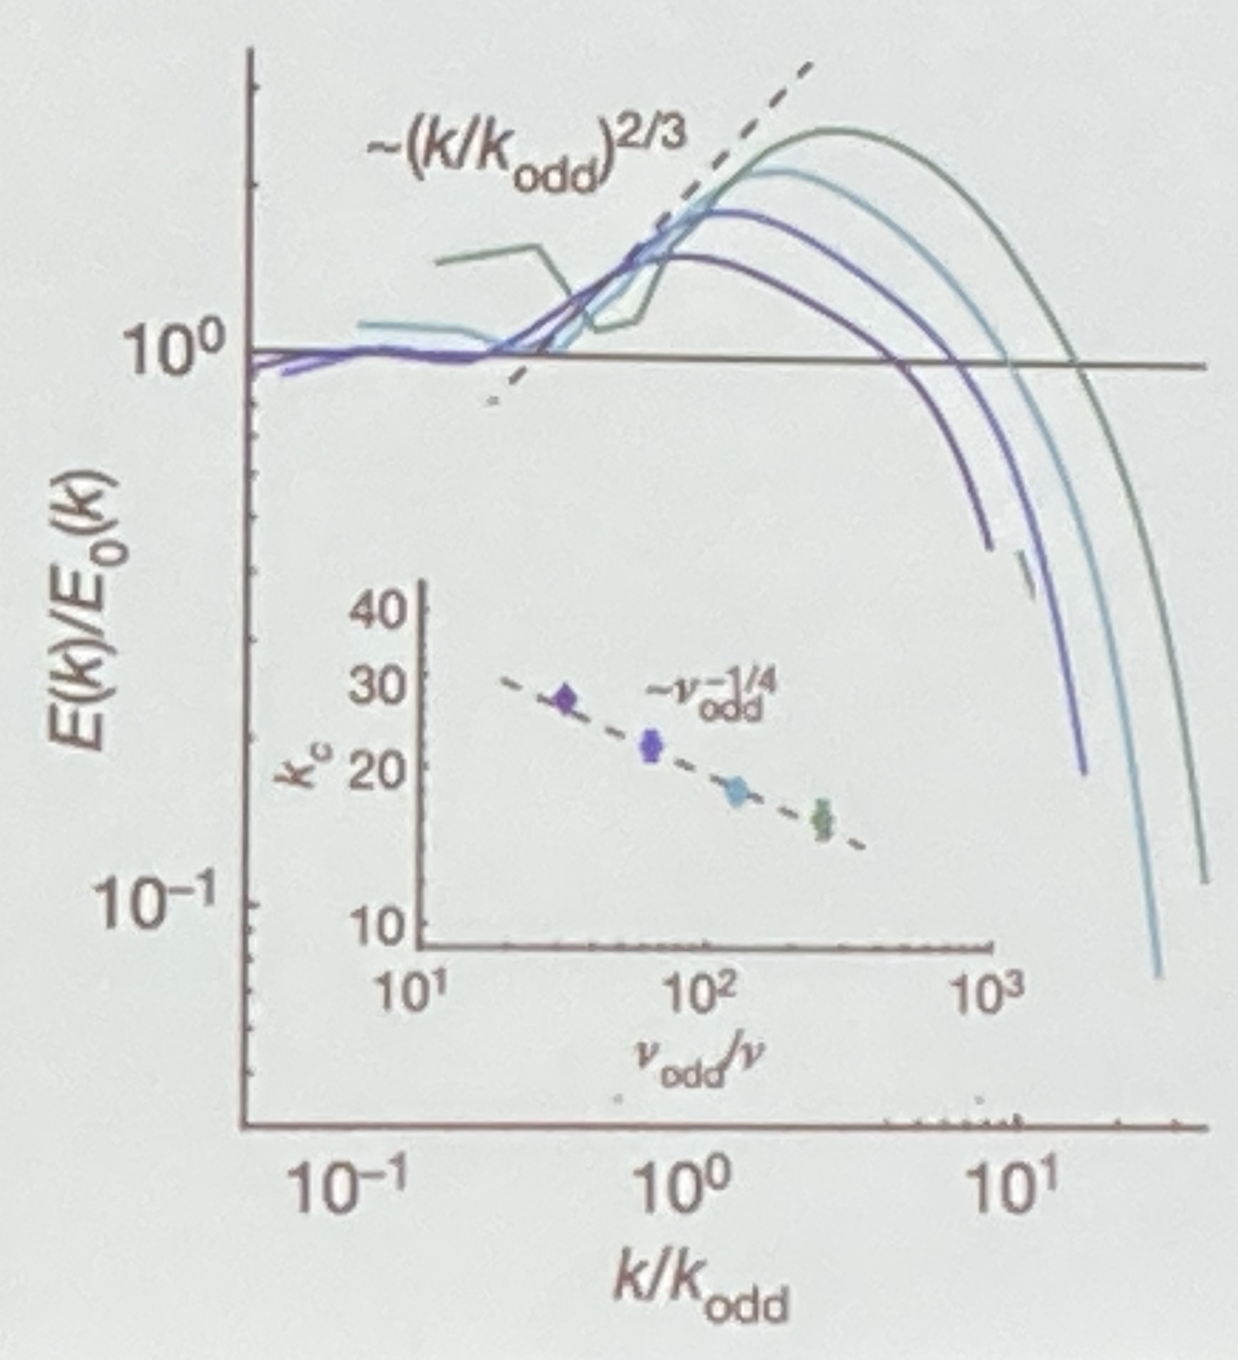
\includegraphics[scale=0.3]{Lectures/Images/lec16-nuscaling.png}
\end{center}

The theory underlying this is that we have pattern formation from two energy fluxes meeting at a particular characteristic lengthscale. Another takeaway - we have a system that behaves as 3D in low $k$, behaves as 2D in high $k$ (and displays a mixed cascade) and the interplay gives rise to some interesting phenomenology. Thus concludes our discussion of turbulence!

This lecture covers what you need for problem 1 of the homework. On Monday we do a problem solving session for problem 2. In the last lecture, we study pattern formation and phase transitions, giving you the tools for problem 3.
\section{Non-reciprocal Phase Transitions}

\subsection{Overview}
We will start by studying scalar active fluids, which is the ``Ising model'' of fluid physics where things are simple but we can see interesting phenomena. We then will qualitatively describe MIPS (motility induced phase separation). We then review some statistical physics and discuss Brownian motion. We then discuss the process of course-graining - going from microscopic physical laws to hydrodynamic equations. We will then derive the Fokker-Planck equation. We will then go back and discuss the microscopic models involved in describing the scalar active fluid. Finally, we will return to MIPS and describe it quantitatively!

\subsection{Describing Fluids}
In this class, we have largely taken a hydrodynamic perspective - forgetting about the fast degrees of freedom and focusing on the slow, large/long-timescale behaviour of the system. In the hydrodynamic perspective, the ``slow variables'' come in two forms:
\begin{itemize}
    \item Conserved quantities: like mass, momentum, energy, and charge.
    \item Broken symmetries: these act as order parameters to classify the phase of matter we are looking at. They are usually packaged in the form of a tensor. Polar active fluids, nematics, chiral fluids etc. have associated OPs that describe the phase.
\end{itemize}

Fluids can be generally described by their symmetry group.

\begin{table}[htbp]
    \centering
    \begin{tabular}{|c|c|c|}
        \hline Fluid & Symmetry Group & Order Parameter
        \\ \hline Simple & $O(2)$ (arbitrary reflections/rotations) & $\rho$ (density, scalar)
        \\ Chiral fluids & $SO(2)$ (arbitrary rotations, not reflections) & $\rho_\omega$ (density, pseudoscalar - changes under reflection)
        \\ Polar fluids & $C_1$ ($2\pi n$ rotations) & $P_i$ (momenta)
        \\ Nematics & $C_2$ ($\pi n$ rotations) & $Q_{ij}$ (rank 2-tensor)
        \\ $k$-atics  & $C_k$ ($\frac{2\pi n}{k}$ rotations) & $Q_{i_1, \ldots i_k}$ (rank $k$-tensor)
        \\ \hline
    \end{tabular}
\end{table}

\begin{center}
    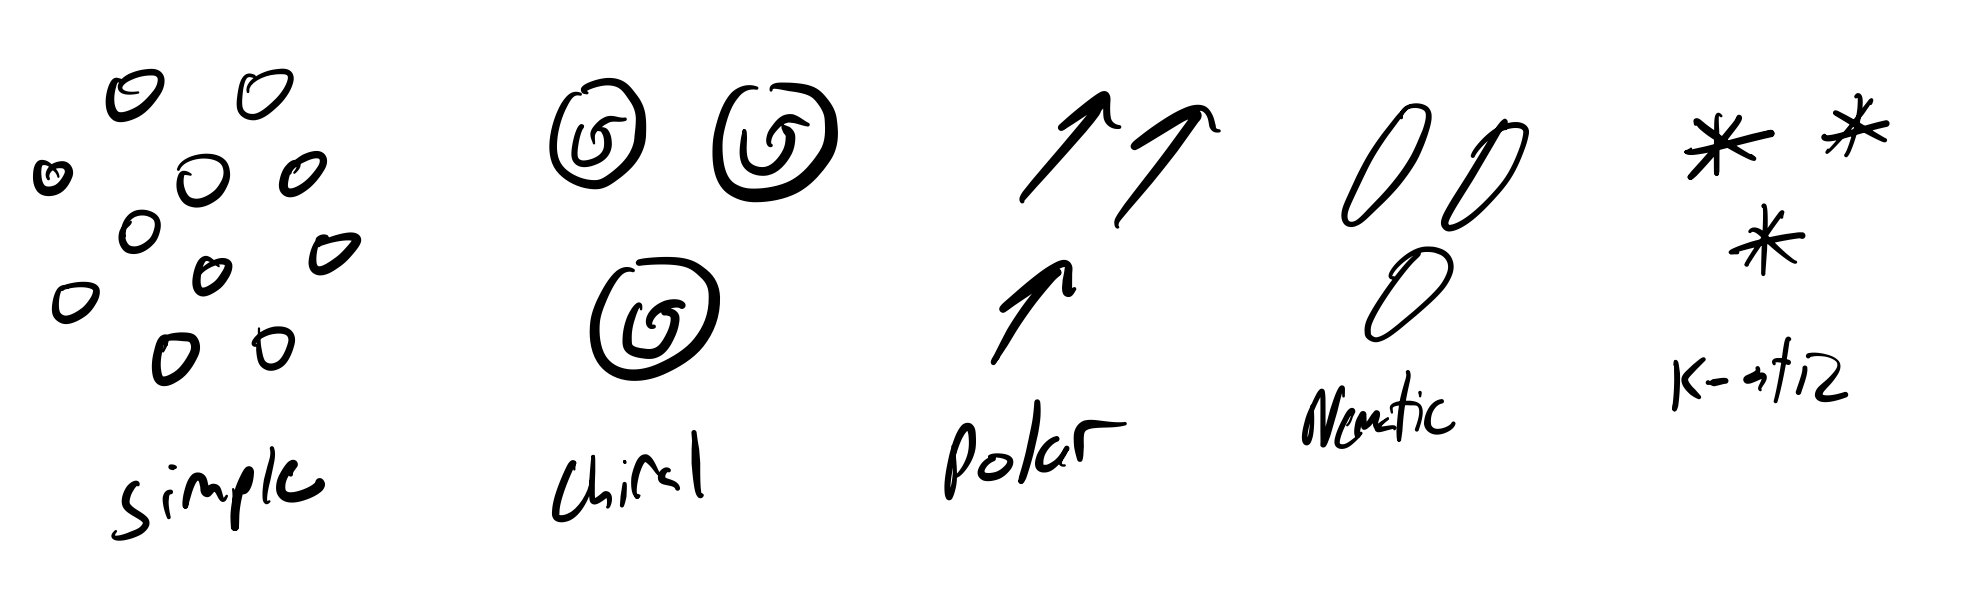
\includegraphics[scale=0.4]{Lectures/Images/lec17-particles.png}
\end{center}

\subsection{MIPS (qualitatively)}
Today we will study scalar active fluids - for such fluids, injecting energy at the microscopic scale for such fluids gives us motility-induced phase separation, or MIPS\footnote{A video of which can be found here \url{https://www.youtube.com/watch?v=H0kou04dylE}}. 

If we just have a box of gas, the probability that they may spontaneously form a water droplet is vanishingly small. In order to get such phase separation in a passive fluid, we need attraction in between molecules, so that the energy associated with them being together is greater than the entropy gain associated with them being farther apart. But interestingly, for active fluids we spontaneously have phase separation, with only repulsive interactions.

We need two ingredients for MIPS:
\begin{itemize}
    \item Repulsive interactions of some form.
    \item Self-propulsion. However, unlike the Viczek model we discussed a couple weeks ago, there is no preferred orientation of the fluid. Each individual particle has an individual polarity, but the fluid as a whole has a total polarity of zero.
\end{itemize}

Qualitatively, how can we see MIPS arise? 
\begin{enumerate}
    \item We first observe (tautologically) that particles spend more time in regions where they move slower.
    \item Particles move slower when their motility is cancelled out by a pairwise collision.
    \item Such particles make a bigger/better target in phase space for other particles to collide with; this target will be stationary. This causes more particles to accumulate. Note that after we form such a region, only particles as the boundaries of such regions have a chance of escaping.
\end{enumerate}

Let's see if we can see MIPS arise quantitatively. We start by reviewing Brownian motion.

\subsection{Brownian Motion and Langevin Dynamics}
We start with a review of classical equilibrium Brownian motion, and then add activity.

Scottish Botanist Robert Brown (1827) noticed pollen grains jiggled; he noticed that a repeated experiment with dead particles still jiggled, so such motion was not due to life. 

Then, many decades later, Albert Einstein (1905) used a course-grained description to derive some properties of Brownian motion:
\begin{equation}
    \frac{\overline{x^2}}{2t} = D = \frac{RT}{6\pi \eta r N_A}
\end{equation}

with $D$ the diffusion coefficient, $R$ the gas constant, $T$ the temperature, $\eta$ the viscosity, $r$ the radius of the spheres, $N_A$ Avogadro's constant. This made a connection between a particle diffusing via Brownian motion and atomic physics, allowing people to estimate the atomic length scale and the amount of atoms in a mole $N_A$.

Marian Smoluchowski gave an idealized argument for why Brownian particles stay in motion.

Finally (though there are many others that worked on this area) Paul Langevin bravely wrote down a (stochastic) differential equation for the motion of an individual diffusing particle. He was also a cool dude\footnote{He was an outspoken anti-fascist, was removed from his position under Nazi rule, but fortunately survived to see the liberation of Paris.}

Let's first think about our favourite dimensionless constant, the Reynolds number:
\begin{equation}
    \text{Re} = \frac{\rho u L}{\eta}
\end{equation}

\begin{center}
    \includegraphics[scale=0.4]{Lectures/Images/lec17-colloid.png}
\end{center}

If we have $L \sim 10\mu\si{m}, m \sim 10\mu\si{m s^{-1}}, \eta/\rho \sim 10^{-6}\si{m^2s^{-1}}$, then the Reynolds number is $\text{Re} \sim 10^{-4} \ll 1$, so We can take the Navier Stokes equation:
\begin{equation}
    \rho D_t\v{v} = \eta \nabla^2 \v{v} - \nabla p + \v{F}_{\text{body}}(\v{r})
\end{equation}
and set the inertial term to zero (Stokes' regime)
\begin{equation}
    0 = \eta \nabla^2 \v{v} - \nabla p + \v{F}_{\text{body}}(\v{r})
\end{equation}
We can then use this to derive the drag force on a sphere moving through fluids using Green's function methods:
\begin{equation}
    F_{\text{drag}} = -6\pi \eta r U
\end{equation}

\begin{center}
    \includegraphics[scale=0.4]{Lectures/Images/lec17-stokesdrag.png}
\end{center}

The net force on the pollen grain is then (using Newton's second law):
\begin{equation}
    m\dod{U}{t} = F_{\text{drag}} + F_{\text{collisions}}
\end{equation}
Or defining $\Gamma = \frac{6\pi \eta r}{M}$:
\begin{equation}
    \boxed{\dod{U}{t} = -\Gamma U + L(t)}
\end{equation}
where $L(t) = F_{\text{collisions}}/m$, is a strongly, quickly fluctuating stochastic term. This is the Langevin equation. So we have a drag term corresponding to exponential decay, in addition to a stochastic term that is sampled every moment in time from an ensemble. Often, people assume that the noise term is drawn from a Gaussian distribution:
\begin{equation}
    \overline{L(t)} = 0
\end{equation}
\begin{equation}
    \overline{L(t)L(t')} = 2\gamma\delta(t-t')
\end{equation}
with $\gamma$ being the fluctuation strength. The $\delta$ correlations means that there is no memory, and the solution will hence be a Markov process - there will be no dependence on the current state of the system on past moments.

Again neglecting the inertial term/making a further approximation, we get the equation for Brownian dynamics:
\begin{equation}
    U(t) = \frac{1}{\Gamma}L(t)
\end{equation}

Note that $\gamma$ can be sometimes obtained from the microscopic physics, but oftentimes it is a phenomelogical paramter for us to figure out.

% The Langevin equations we have written down is pretty poorly defined if we think about it too hard (we need tools developed by Stratonovich and Ito)

\subsection{Course-Graining}
We want a process of going from individual microcopic trajectories to an ensemble/probability distribution:
\begin{equation}
    X(t) \to \set{X(t)} \to P(X, t)dX
\end{equation}
the result will be a Fokker-Planck equation:
\begin{equation}
    \dpd{P(X, t)}{t} = \ldots
\end{equation}
There is not a unique way to coarse grain a generic stochsastic system, because different people are interested in different things, and coarse graining involves making certain approximations/throwing away information. But for Langevin:
\begin{equation}
    \dod{X}{t} = a(X) + bL(t)
\end{equation}
we have that this exactly coarse grains into:
\begin{equation}
    \dpd{P(X, t)}{t} = -\dpd{[a(X)P]}{X} + \gamma\dpd[2]{[b^2P]}{X}
\end{equation}

More generally, coarse graining can be studied by the derivation of the Dean equation; namely, if we have:
\begin{equation}
    \frac{\text{d}\v{R}^{\alpha}}{\text{d}t} = \sum_{\beta=1}^{N}\v{F}(\v{R}^\alpha(t) - \v{R}^{\beta}(t)) + \v{G}(\v{R}^{\alpha}(t)) + \gv{\eta}^\alpha(t)
\end{equation}
Where:
\begin{equation}
    \xi^\alpha_i(t)\xi^\beta_j(t') = 2T\delta_{ij}\delta^{\alpha\beta}\delta(t-t')
\end{equation}
We have the density:
\begin{equation}
    \rho(\v{R}, t) = \sum_{\alpha=1}^N\delta(\v{R}^\alpha(t) - \v{R})
\end{equation}
And through a course graining procedure, we obtain the Dean equation:
\begin{equation}
    \dpd{\rho}{t} = T\nabla^2 \rho - \nabla \cdot \left[\v{G}(\v{R})\rho(\v{R}, t) + \int d^d \v{R}'\v{F}(\v{R} - \v{R}')\rho(\v{R}, t)\rho(\v{R}', t)\right] + \gv{\eta}(\v{R}, t)
\end{equation}
where $\gv{\eta}(\v{R}, t)$ is a stochastic field sastisfying
\begin{equation}
    \eta(\v{R}, t)\eta(\v{R}', t') = 2T \delta_{ij}\delta^{(d)}(\v{R} - \v{R}')\delta(t-t')
\end{equation}
As you have time, it is recommended to look at problems 3.10 (deriving Dean equation), 3.11 (deriving the Fokker-Planck equation from Dean), 9.2 (deriving the Toner-Tu equations from Dean). so you can see this machinery in detail. These are some of the most challenging problems in the book, but are worth doing!

We also introduce the master equation; this is the most general equation we could write to desribe the time evolution of a probability density. Labelling the states by $n$:
\begin{equation}
    \dot{P}_n(t) = \sum_{n'}W_{n'\to n}P_{n'}(t) - W_{n\neq n'}P_n(t)
\end{equation}
Where detailed balance is given by:
\begin{equation}
    W_{n'\to n}P^{\text{eq}}_n = W_{n\to n'}P^{\text{eq}}_{n'}
\end{equation}

For hopping on a 1D lattice:
\begin{equation}
    W_{n \to n'} = 0 \text{ unless } n' = n \pm 1 \quad \text{locality}
\end{equation}
\begin{equation}
    \begin{split}
        W_{n + 1 \to n} &= W_{n'+1 \to n'} = W_{\text{left}}
        \\ W_{n - 1 \to n} &= W_{n'-1 \to n'} = W_{\text{right}} \quad \text{(homogeneity)}
    \end{split}
\end{equation}
\begin{equation}
    W_{\text{left}} + W_{\text{right}} = 1 \quad \text{(unitarity)}
\end{equation}
Writing $W_{\text{right}} = \frac{1}{2} + \e, W_{\text{left}} = \frac{1}{2}-\e$, we get:
\begin{equation}
    \dot{P}_n = \left(\frac{1}{2} - \e\right)P_{n+1} + \left(\frac{1}{2} + \e\right)P_{n-1} - P_n = \frac{P_{n+1} - 2P_n + P_{n-1}}{2} - \e(P_{n+1} - P_{n-1}) = \frac{1}{2}\dpd[2]{P_n}{n} - \e\dpd{P_n}{n}
\end{equation}
Replacing $n = xa$ with $a$ the lattice spacing, then we arrive at the Fokker-Planck equation! This is in some sense the classical analog of the Schrodinger equation.

\subsection{MIPS (quantitatively)}
We consider two different models; the first is the active Brownian particle model:
\begin{equation}
    \dod{\v{r}_n}{t} = v_0\hat{\v{u}}(\theta_n) - \frac{1}{\gamma}\sum_{m\neq n}\nabla_n V(\v{r}_m - \v{r}_n)
\end{equation}
\begin{equation}
    \dod{\theta_n}{t} = \sqrt{2 D_\theta}\eta_n
\end{equation}
where:
\begin{equation}
    \overline{\eta_m(t)\eta_{n}(t')} = \delta_{mn}\delta(t-t')
\end{equation}

We also have the run-and-tumble model:
\begin{equation}
    \dod{\theta_n}{t} = \begin{cases}
        \sqrt{2D_\theta}\eta_n & \text{if } \abs{t - nT} < \e
        \\ 0 & \text{otherwise}
    \end{cases}
\end{equation}

The difference between the two models just being that either the noise is continuous or the particles run, and then stochastically rotate. ABPs well-describe colloids, while RTPs well-describe bacteria. Both give the same Fokker-Planck equation (the starting point ot your homework):
\begin{equation}
    \p_t P(\v{r}, \theta, t) = -\hat{\v{u}}(\theta)\cdot \nabla[\v{v}(\v{r})P(\v{r}, \theta, t)] + D_\theta\p_\theta^2P(\v{r}, t, \theta)
\end{equation}

and both give rise to MIPS dynamics. The ending point of your homework is as follows; you do a linear stability analysis on the fields, and find that the fluctuations of the fourier modes evolve as:
\begin{equation}
    \p_t \delta \rho(\v{q}, t) = -\frac{v(\rho_0)}{2D_\theta}[v(\rho_0) + \rho_0\left.\dpd{v}{\rho}\right|_{\rho_0}]q^2\delta \rho(\v{q}, t)
\end{equation}
The only thing that could be negative is the derivative term, and this gives the quantiative picture of MIPS based on stability based on whether this term changes sign. If you want to read more about this, check out chapter 8 on the spinoidal decomposition.

\subsection{References}
\begin{itemize}
    \item A minimum of stochastics for Scientists (Noel Corngold)
    \item Active Matter: from motility to self-organization, Boulder school on Self-organizing matter July 2024 (M. Cristina Marchetti) - check out part 3 for help with the homework.
\end{itemize}

\section{Pattern Formation \& Non-Reciprocal Phase Transitions}

In stat mech, we generally understand a phase transition as a discontinuity in a free energy, or where the free energy of a system changes form (e.g. from a single to a double well). How do we understand phase transitions in systems where we cannot write down an energy?

\subsection{Swift-Hohenberg Model}
We consider the dynamical equation (a non-linear PDE):
\begin{equation}\label{eq:swifthohen}
    \p_t u(x, t) = ru - (1 + \lambda_c^2\nabla^2)^2u - u^3
\end{equation}
What the $\lambda_c^2 \nabla^2$ term does is favour the system towards an oscillation a wavelength $\lambda_c$. It is easy to reinterpret this equation as the variation of a potential:
\begin{equation}
    \p_t u = -\frac{\delta V}{\delta u}
\end{equation}
Where:
\begin{equation}
    V = \int dx \left(-\frac{1}{2}ru^2 + \frac{1}{4}u^4 + \frac{1}{2}\left[[\lambda_c^2 \nabla^2 + 1]u\right]^2\right)
\end{equation}
where in we see the $\lambda_c$ term vanishes if we consider $u = e^{iqx}$ with $q = \frac{1}{\lambda_c}$. But note that Eq. \eqref{eq:swifthohen} has an additional solution, namely $u = 0$.

To this end, we have to do a linear stability analysis around the solutions (we skip some steps - this is done in the text and also in your homework), and see if the perturbation grows or decays in time. So, we consider:
\begin{equation}
    u = u_0 + \delta u(x, t) = \delta u(x, t)
\end{equation}
where we have taken the $u_0 = 0$ solution. We can now linearize around the perturbation:
\begin{equation}
    \p_t \delta u = L\delta u + O((\delta u)^2) = \underbrace{[r - (1 + \lambda_c^2\nabla^2)^2]}_{L}\delta u + O((\delta u)^2)
\end{equation}
If we Fourier transform the $L$:
\begin{equation}
    L(q) = [r - (1 - q^2\lambda_c^2)^2]
\end{equation}
We can now write down the exponential behaviour of $\delta u(q)$:
\begin{equation}
    \delta u(q) = e^{\sigma(q) t}
\end{equation}
where:
\begin{equation}
    \sigma(q) = (r - 1) + 2\lambda_c^2 q^2 - q^4\lambda_c^4
\end{equation}
So - we are interested in the sign of $\sigma(q)$, because if $\sigma(q)$ is negative then $u$ is stable ($\delta u \to 0$), and if $\sigma(q)$ is positive then $u$ is unstable ($\delta u \to \infty$). To this end, let us plot $\sigma(q)$, which will be a symmetric function around $q = 0$:

\begin{center}
    \includegraphics[scale=0.3]{Lectures/Images/lec18-sigmaq.png}
\end{center}

We find at the maxima:
\begin{equation}
    \sigma(\tilde{q} = \pm 1) = (r - 1) + 2 - 1 = r
\end{equation}
So depending on the sign of $r$, we have stability or instability, with wavelength selection at $\tilde{q} = 1$ or at $q_c = \frac{1}{\lambda_c}$.

If we study perturbative solutions to Eq. \eqref{eq:swifthohen}, we find:
\begin{equation}
    u(x, t) = \underbrace{a_1}_{\sqrt{\frac{4}{3}r}}\cos(x) + \mathcal{O}(r^{3/2})\cos(3x)
\end{equation}
Much like in critical phenomena we expand in $T - T_c$, we here expand in $r$. We can look at the amplitude of the $u$:

\begin{center}
    \includegraphics[scale=0.35]{Lectures/Images/lec18-ux.png}
\end{center}

Where we find a pitchfork bifurcation:

\begin{center}
    \includegraphics[scale=0.35]{Lectures/Images/lec18-Abifurcation.png}
\end{center}

Much like you have seen in the Ising model. How do we understand this? We are looking at the solutions:
\begin{equation}
    u(x, t) \sim A(x, t)e^{iq_c x} + \text{c.c.}
\end{equation}
where $e^{iq_c x}$ is dictated by the fastest growing mode. We have oscillation dictated by $q_c$, but we can also have a modulation of the amplitude (slower than dictated by $q_c$) dictated by $A(x, t)$, giving a more full description of the problem:

\begin{center}
    \includegraphics[scale=0.35]{Lectures/Images/lec18-Amodulation.png}
\end{center}

What we can do is consider a complex amplitude $A = ae^{i\phi}$ (with $a = \abs{A}$) and consider a shift to the phase:
\begin{equation}
    \phi \to \phi + \Delta \phi
\end{equation}

\begin{center}
    \includegraphics[scale=0.35]{Lectures/Images/lec18-phasediff.png}
\end{center}

This causes a translation of the pattern in time (known as limit cycles). Notice that in our model we have a transition from no pattern (in our case at $r < 0$ where $A = 0$) to a periodic pattern (at $r > 0$ where $A = \pm\sqrt{r}$) - spontaneous translational symmetry breaking - controlled by $r$.

\subsection{Non-reciprocal Swift-Hohenberg Model}
We want to introduce non-reciprocity into our model. We do this by introducing two fields labelled by $a = 1, 2$ and modify the $r$ coefficient to be a matrix $\e_{ab}$, so our dynamical equation becomes:
\begin{equation}
    \p_t u_a(x, t) = \e_{ab}u_b - (1 + \lambda_c^2\nabla^2)^2u_a - u_a^3
\end{equation}
Now, we notice that if $\e_{ab} \neq \e_{ba}$, it is the case that:
\begin{equation}
    \p_t u \neq -\frac{\delta V}{\delta u}
\end{equation}
because the antisymmetric part of $\e_{ab}$, i.e.:
\begin{equation}
    \e_{ab}^o = - \e^o_{ba}
\end{equation}
then:
\begin{equation}
    \e^o_{ab}u_a u_b = 0
\end{equation}
(as we multiply an antisymmetric object with a symmetric one) so while $\e_{ab}u_b$ can exist as a term in the equation of motion, there is no way of writing this down in the potential.

Note that without the cubic term, we would have just an equation of motion that describes a 1-D crystal. But the cubic/nonlinear term allows us to describe the transition between a 1-D crystal and no crystal formation.

We consider:
\begin{equation}
    \e =\m{\e_{11} & \e_{12} \\ \e_{21} & \e_{22}} =  \m{\e_{0} & \e_{12} \\ \e_{21} & \e_0}
\end{equation}
Now, let us write:
\begin{equation}
    \e_{12} = \e_+ + \e_-
\end{equation}
\begin{equation}
    \e_{21} = \e_+ - \e_-
\end{equation}
i.e. writing the off-diagonal components of the tensor in terms of the symmetric and antisymmetric parts. Now let us write:
\begin{equation}
    u_a(x) = A_a(x)e^{ik_c x} + \text{c.c.}
\end{equation}
Which allows us to write the equations of motion for $A_a$:
\begin{equation}
    \p_t A_1 =  \e_0 A_1 + \e_{12}A_2 - g\abs{A_1}^2A_1
\end{equation}
\begin{equation}
    \p_t A_2 = \e_0 A_2 + \e_{21}A_1  - g\abs{A_2}^2A_2
\end{equation}
which we can either derive or argue from symmetry considerations based on the equation of motion for $u$. 

We work in the regime where:
\begin{equation}
    \e_0 \gg \e_- \gg \e_+
\end{equation}

If we simulate this, we find that $u_1, u_2$ move with the same velocity if they are off by a phase. If the phase offset is zero, the pattern is fixed. So, the model allows for three cases - states where the patterns do not form, states where patterns form but they are static, and states where the pattern form and are dynamic; they spontaneously break the symmetry and move together the left/right.

\begin{center}
    \includegraphics[scale=0.3]{Lectures/Images/lec18-wavedynamics.png}
\end{center}

Let us look at the steps of the calculation to figure out the phase diagram of this model (you will flesh out the steps in the homework).

\subsection{Deriving the Motion/Phase Diagram}
Let us write:
\begin{equation}
    A_1 = a_1e^{i\phi_1}
\end{equation}
\begin{equation}
    A_2 = a_2e^{i\phi_2}
\end{equation}
And plug them into our coupled differential equations for $A_1, A_2$. If we then parameterize:
\begin{equation}
    \Delta \phi = \phi_2 - \phi_1,\quad \bar{\phi} = \phi_2 + \phi_1
\end{equation}
where $\Delta \phi$ is the phase difference, $\bar{\phi}$ is the mean of the phases. We find a beautiful set of equations (to leading order in $\Delta \phi$):
\begin{equation}
    \p_t \Delta \phi = \alpha \Delta \phi - \beta \Delta \phi^3
\end{equation}
\begin{equation}
    \p_t \bar{\phi} = \gamma \Delta \phi
\end{equation}
where you will also derive how $\alpha, \beta, \gamma$ depend on $\e_{ab}$:
\begin{equation}
    \alpha = 2[\e_-^2 - \e_+\e_0]/\e_0
\end{equation}
\begin{equation}
    \gamma = 2\e_-
\end{equation}
and $\beta > 0$. Note that without linearization, the second equation would read $\p_t \bar{\phi} = \gamma \sin(\Delta \phi)$ so we have indeed linearized. 

If we look at the first equation, we have standard pitchfork bifurcation; indeed the set of equations for $\Delta \phi, \bar{\phi}$ is known as \emph{drift pitchfork bifurcation}.

Let's look at stable solutions to the first equation:
\begin{equation}
    0  = \alpha\Delta \phi - \beta \Delta \phi^3 = \Delta\phi(\alpha - \beta\Delta \phi^2)
\end{equation}
so we have solutions:
\begin{equation}
    \Delta \phi = 0, \Delta \phi = \pm\sqrt{\frac{\alpha}{\beta}}
\end{equation}
When $\alpha < 0$, we only have the $\Delta \phi = 0$ solution, and when $\alpha > 0$ we have that the $\pm\sqrt{\frac{\alpha}{\beta}}$ are the minima.

Looking at the second equation, for $\Delta \phi = 0$ we have that $\p_t \bar{\phi} = 0$ (so no motion of the mean) while for $\Delta \phi = \pm\sqrt{\frac{\alpha}{\beta}}$ we have motion of the mean to the right/left. The absolutely crucial thing to notice here is that if we view the motion of $\m{\Delta \phi & \bar{\phi}}^T$, the first component alone may admit a variational structure (as you have seen with magnetization in the Ising model), but together they do not admit such a structure! Also note that the dynamics here manifestly break the mirror symmetry - the dynamics are chiral.

If we linearize, we have the matrix form:
\begin{equation}
    \p_t \m{\Delta \phi \\ \bar{\phi}} = \m{\alpha & 0 \\ \gamma & 0}\m{\Delta \phi \\ \bar{\phi}}
\end{equation}

We have the phase diagram:

\begin{center}
    \includegraphics[scale=0.35]{Lectures/Images/lec18-phasediagram.png}
\end{center}

We can study the exceptional points; namely as $\alpha \to 0$ the eigenvectors of $\m{\alpha & 0 \\ \gamma & 0}$ coalesce/become collinear. (Why is the second column always zero? $\bar{\phi}$ corresponds to a uniform translation of the pattern, and it never plays a role in determining the phase difference $\Delta \phi$). Note that whenever we diagonalize this matrix, we have one eigenvalue that is always zero, which corresponds to the Goldstone mode. But at the exceptional point the other (nonzero) eigenvalue becomes zero, and that is where the transition happens. The onset of the bifurcation occurs at the exceptional point of the Jacobian, and then we can derive the phase diagram of this system.

\subsection{Non-Reciprocal Flocking Models}
Although it is more complicated, we can also see such a non-reciprocal phase transition arise in a Flocking model - we can take the Vicsek model, add two types of populations, and make their interactions non-reciprocal. Unlike the standard Vicsek model where the flock travels in a particular direction uniformly, in the non-reciprocal model we have that the two populations rotate, with the order parameters rotating, with a fixed angle/phase difference $\Delta \phi$ between them. If $\Delta \phi = 0$ then we just have flocking (alignment - static phase), same if $\Delta \phi =\pi$ (antialignment - static phase) and if we have in between, then we have the chiral phase. Therein we see a similar structure emerging as the non-reciprocal Swift-Hohenberg model. We can also look at the frequency of the rotation, and the larger the $\Delta \phi$ is (away from $\Delta \phi = 0, \pi$) the quicker the rotation.

\begin{center}
    \includegraphics[scale=0.3]{Lectures/Images/lec18-flocking.png}
\end{center}
\begin{center}
    \includegraphics[scale=0.35]{Lectures/Images/lec18-flockingphases.png}
\end{center}

\subsection{Goldstone Modes, Comments on Non-Reciprocal Phase Transitions}

Note that in this problem we also have a Goldstone mode - a global rotation (the analog of translation on a line - here we have just put the entire system on a ring, so the translational Goldstone mode becomes a global rotational Goldstone mode). Usually, people talk about Goldstone modes as the rotation around the Mexican hat (here $\bar{\phi}$) and the oscillatory mode as the massive one (here $\Delta \phi$). At the exceptional point, the massive mode coalesces with the Goldstone one. 

\begin{center}
    \includegraphics[scale=0.3]{Lectures/Images/lec18-goldstone.png}
\end{center}

Normally, people think about equilibrium phases as performing an optimization with $\p_t \phi = -\frac{\delta F}{\delta \phi}$. But, non-equilibrium forces also have a transverse component, and therein the cyclic dynamical states do not arise from any free energy minimization/variational mechanics. 

\begin{center}
    \includegraphics[scale=0.3]{Lectures/Images/lec18-nonvariational.png}
\end{center}

Such non-variational systems are quite ubiquotous, e.g. in biological systems, social dynamics or open quantum systems (where we lose unitarity) - indeed, most systems are, despite what the concentration of papers focusing on equilibrium systems may indicate.

\end{document}